% \documentclass[conference]{report}

\documentclass[12pt]{article}

\usepackage{preamble}

\begin{document}

\title{\huge MAE 541 Final Project Paper}

\author{Jannik Gräbner\footnote{PhD candidate, jg3607@princeton.edu}, Jack Sydney Schwartz \footnote{PhD student, js1765@princeton.edu}, Claudio Vestini \footnote{Visiting undergraduate student, claudio.vestini@keble.ox.ac.uk} \\
\textit{\normalsize Mechanical \& Aerospace Engineering} \\
\textit{\normalsize Princeton University} \\
% \normalsize Princeton, NJ, United States of America}
\normalsize Princeton, NJ}

\date{8 May 2026}

\maketitle

%\begin{abstract}
%    As interest in the Earth-Moon domain grows, the risk of orbital debris generation grows correspondingly. 
%    Unlike debris in near-Earth dynamics, natural removal is extremely limited. 
%    Moreover, the dynamics are dominated by multi-body effects that make traditional propagation methods inadequate. 
%    In this work, we introduce a novel framework with the potential to improve the analysis of long-term propagation of debris in this domain.
%    At this preliminary stage, we assume the dynamics to be well approximated by the circular restricted three-body problem. 
%    By partitioning the phase space into neighbourhoods of periodic orbit crossings, the local application of applied dynamical systems tools (such as normal form theory), is used to more efficiently propagate orbits in various energy domains. \textcolor{red}{\textbf{COULD POSSIBLY ALTER OR REMOVE ABSTRACT ALL TOGETHER}}
%\end{abstract}

\tableofcontents

\section{Introduction} \label{sec:introduction}

\textcolor{red}{INTRODUCTION}

\begin{figure}[h]
    \centering
    \includegraphics[width=\linewidth]{Figures/ONECOL_FIGURE.jpg}
    \caption{\textcolor{red}{ONECOL FIGURE CAPTION}.}
    \label{fig:SAMPLE_ONECOL_FIGURE}
\end{figure}

\begin{figure*}
    \centering
    \begin{subfigure}[t]{0.49\textwidth}
        \centering
        \includegraphics[width=0.9\textwidth]{Figures/TWOCOL_FIGURE1.pdf}
        \caption{\textcolor{red}{TWOCOL FIGURE 1 SUBCAPTION}.}
        \label{fig:SAMPLE_TWOCOL_FIGURE1}
    \end{subfigure}
    \hfill
    \begin{subfigure}[t]{0.49\textwidth}
        \centering
        \includegraphics[width=0.9\textwidth]{Figures/TWOCOL_FIGURE2.pdf}
        \caption{\textcolor{red}{TWOCOL FIGURE 2 SUBCAPTION}.}
        \label{fig:SAMPLE_TWOCOL_FIGURE2}
    \end{subfigure}
    \caption{\textcolor{red}{TWOCOL FIGURE CAPTION}.}
    \label{fig:SAMPLE_TWOCOL_FIGURE}
\end{figure*}

\section{The Circular Restricted Three Body Problem} 
\label{sec:CR3BP}

Our project studies the dynamics of the Earth--Moon CR3BP. A simplification of the more general Three-Body Problem (3BP), this continuous-time, non-integrable dynamical system is one of the most celebrated and extensively studied in the history of both mathematics and physics. It is, in fact, through the analysis of this very system that French mathematician Henri Poincaré gave birth to the fields of dynamical systems and chaos theory, the fundamental tenets of our MAE 541 course.

\subsection{A Brief Historical Summary} \label{subsec:history}

Although problems in astrodynamics have forever inspired humankind and his discoveries, the first recognizable mathematical formalization of the general 3BP appeared in the XVII century \emph{Principia Mathematica} by Isaac Newton \cite{newton1687principia}. After successfully inventing the mathematical framework to generalise previous findings on the Two-Body problem (i.e. the Keplerian orbits and Kepler's laws), Newton elegantly derived the dynamics of the Earth--Moon--Sun system, and attempted to find admitted closed-form solutions, without success. In conversations with his contemporary Dr Edmond Halley, who was pressing Newton to finish his work on 3BP theory, he admitted that studying this system ``made [his] head ache, and kept [him] awake so often, that [he] would think of it no more" \cite{brewster1855memoirs}.

Newton's work was picked up in the 1760's by Leonhard Euler, who took the first major steps toward the simplification of the general problem to the familiar CR3BP form. He did so by introducing a \emph{synodic}, or rotating, coordinate system that moved along with the two \emph{primary} bodies. Euler was also the first to search for specific configurations where a third, \emph{secondary} body could remain fixed relative to the two primaries, discovering the first three collinear equilibrium points \cite{euler1767motu}.

A comprehensive mathematical formalization of the restricted assumption came from Joseph-Louis Lagrange in his 1772 \emph{Essai sur le problème des trois corps} \cite{lagrange1772essai}. Lagrange posited a system where two primary bodies of finite mass move in circular orbits around their common centre of mass, while a third body of negligible mass is attracted to the two primaries without any measurable effect on the gravitational environment. On top of Euler's collinear points, Lagrange discovered two additional triangular equilibrium points. As a result, today all five equilibrium (or \emph{libration}) points of the CR3BP are universally referred to as the Lagrange (or $\mathcal{L}$) points. For decades to follow, mathematicians searched for integrals of motion that would allow the differential equations to be solved. In 1836, Carl Gustav Jacob Jacobi formulated the existence of the first integral of motion of the problem, the Jacobi Constant, which remains the only known conserved quantity in the CR3BP \cite{jacobi1836mouvement}. Using this constant, Jacobi also introduced zero-velocity surfaces defining topological boundaries for where the third body is allowed to travel.

The late XIX century marked a profound shift in how the CR3BP was understood. Motivated by an 1887 prize offered by King Oscar II of Sweden for a general mathematical solution to the n-body problem, Henri Poincaré submitted a manuscript focusing heavily on the restricted problem. In this monumental work, Poincaré proved mathematically that the system is non-integrable, thus establishing that a closed-form algebraic solution is impossible \cite{poincare1890sur}. Instead, Poincaré shifted the focus of the analysis towards topological and qualitative dynamics. In so doing, he first discovered \emph{homoclinic tangles}, giving rise to the modern field of chaos theory. In addition, Poincaré was also the first to theorize the existence of an infinite family of periodic orbits admitted by the CR3BP \cite{Poincare_1893}. These were later traced out with the advent of digital computation and numerical methods.

Indeed, most recent contributions have been enabled by the application of modern computational solvers to Poincaré's theory.  At the dawn of the XXI century, researchers were able to identify and map the stable and unstable \emph{invariant manifolds} that branch from periodic orbits \cite{koon2000invariant}, demonstrating their utility for optimal mission design through the \emph{interplanetary transport network}. The 3BP is increasingly receiving attention even outside of the academic sphere: in 2024 the TV-Series \emph{3 Body Problem}, an English language adaptation of a book by Chinese author Liu Cixin, was released and quickly became popular on the streaming site Netflix. To this day, the CR3BP remains an active frontier of scientific research. This simplified system is often used as a preliminary framework for orbital mission design, serving as a bridge between analytical theory and the modern demands of space exploration.

\subsection{Analytical Derivation of System Dynamics} \label{subsec:dynamics_derivation}
\subsubsection{Inertial Frame}
We begin by considering the general 3BP, which studies the dynamics of an isolated system containing three point-mass bodies with position vectors $\bar{\boldsymbol{r}}_{(i)} \coloneq (\bar{x}_{(i)}, \bar{y}_{(i)}, \bar{z}_{(i)})$ and masses $\bar{m}_i$, where $i \in \{1,2,3\}$. Combining Newton's Law of Universal Gravitation with his Third Law, the three masses mutually attract each other according to the equation of motion
\begin{equation*}
    \bar{m}_i \frac{d^2 \bar{\boldsymbol{r}}_{(i)}}{d\bar{t}^2}
    = G \sum_{j\neq i}\frac{\bar{m}_i \bar{m}_j}{\bar{r}_{(ij)}^3}\,\bar{\boldsymbol{r}}_{(ij)}.
\end{equation*}
where $G$ is the Gravitational Constant, $\bar{\boldsymbol{r}}_{(ij)} \coloneq \bar{\boldsymbol{r}}_{(j)} - \bar{\boldsymbol{r}}_{(i)}$ is the relative position of each point-mass $\bar{m}_j$ with respect to $\bar{m}_i$, and $\bar{r}_{(ij)} \coloneq \|\bar{\boldsymbol{r}}_{(ij)}\|_2^2$ is the magnitude of the relative position vector, with $\|\cdot\|_2^2$ being the Euclidean norm in $\mathbb{R}^3$. To simplify the dynamics, in the CR3BP we impose the following assumptions and notation.

A system of natural units is used to normalize position, time, and velocity variables: the distance unit (DU) is the distance between the primary and secondary, the time unit (TU) is the orbital period of the primary and secondary divided by $2\pi$, and the mass unit (MU) is $\bar{m}_1+\bar{m}_2$. Substituting the normalized variables $m_i \coloneq \bar{m}_i / \mathrm{MU}$, $t \coloneq \bar{t}/\mathrm{TU}$, and $\boldsymbol{r}_{(i)} \coloneq \bar{\boldsymbol{r}}_{(i)}/\mathrm{DU}$ and rearranging, we obtain
\begin{equation*}
    m_i \frac{d^2\boldsymbol{r}_{(i)}}{dt^2} = \left( \frac{G \cdot \mathrm{MU} \cdot \mathrm{TU}^2}{\mathrm{DU}^3} \right) \sum_{j\neq i}\frac{m_i m_j}{r_{(ij)}^3}\boldsymbol{r}_{(ij)}.
\end{equation*}
The constant term is the product of terms $G \cdot \mathrm{MU}/\mathrm{DU}^3$ and $\mathrm{TU}^2$. By Kepler's Third Law and definition of the time unit, we have
\begin{equation*}
    \mathrm{TU} = \sqrt{\frac{\mathrm{DU}^3}{G \cdot \mathrm{MU}}}.
\end{equation*}
The constant term thus evaluates to unity, yielding the normalized equations of motion.

To simplify the system even further, we assume that the third body has negligible mass, $m_3 << m_1,m_2$. Consequently, this body does not exert any force on the other two and does not affect their motion. We refer to the larger bodies as the \emph{primary}, $m_1$, and the \emph{secondary}, $m_2$, where $m_1>m_2$. For brevity, we rename the smallest body's normalized mass and normalized position vector $m = m_3$ and $\boldsymbol{r} = \boldsymbol{r}_{(3)}$. In the inertial frame, the simplified, normalized equation of motion for the smallest body is thus given by
\begin{equation} \label{eq:inertial_kinematiks}
    \frac{d^2\boldsymbol{r}}{dt^2} =\frac{d^2\boldsymbol{r}_{(3)}}{dt^2}
    = \frac{m_1}{r_{(13)}^3}\boldsymbol{r}_{(13)}
    + \frac{m_2}{r_{(12)}^3}\boldsymbol{r}_{(12)}.
\end{equation}

We can reduce the number of the system's parameters to just one by defining the \emph{mass ratio} 
\begin{equation} \label{eq:mass ratio}
    \mu \coloneq \frac{m_2}{m_1+m_2}.
\end{equation}
In the normalized system, the mass of the primary $m_1$ is thus $1-\mu$, and that of the secondary $m_2$ is $\mu$.

Our project is primarily focused on the Earth--Moon system; however, using the same normalization framework, the system can model any primary-secondary pair (such as the Sun--Earth system) by simply altering the normalization constants. All reference constants for the Earth--Moon and Sun--Earth system are shown in \cref{tab:cr3bp_parameters}. 

\begin{table}[htpb]
    \centering
    \caption{Normalization constants for the Earth--Moon and Sun--Earth systems in the CR3BP.}
    \label{tab:cr3bp_parameters}
    \begin{tabular}{l c c}
        \hline
        Quantity & Earth--Moon Value & Sun--Earth Value \\
        \hline
        Mass Parameter ($\mu$) & $1.2150582 \times 10^{-2}$             & $3.003 \times 10^{-6}$ \\
        Distance Unit (DU)     & $384,400~\mathrm{km}$    & $1.4960 \times 10^8~\mathrm{km}$\\
        Time Unit (TU)         & $4.348~\mathrm{days}$     & $58.131~\mathrm{days}$ \\
        Mass Unit (MU)         & $6.0458 \times 10^{24}~\mathrm{kg}$ & $1.989 \times 10^{30}~\mathrm{kg}$ \\
        \hline
    \end{tabular}
\end{table}

\subsubsection{Synodic Frame} \label{subsubsec: synodic frame}
To complete the set of assumptions behind the CR3BP, we shift the reference frame from the inertial (fixed) frame, described so far, to a \emph{synodic} (rotating) reference frame. This frame considers the position $P$ of the smallest body $m$.

We denote as $(x,y,z)$ the coordinates of $P$ expressed in the synodic reference frame. We place the origin of our frame at the barycentre of primary and secondary, with the $x$--axis aligned with the line joining these two bodies, oriented in the direction of the secondary $m_2$. The frame is then made to rotate, along with the primary and secondary, around the $z$--axis with constant angular velocity $\omega$ equal to the mean motion of the primaries. Given our normalization, the angular velocity is unitary, and the angular velocity vector is thus given by $\boldsymbol{\omega} = (0,0,1)$. The $y$--axis is set so to complete a right-handed coordinate system.

In this configuration, the primary $m_1$ and secondary $m_2$ are fixed on the $x$--axis at positions $(-\mu, 0, 0)$ and $(1-\mu,0,0)$, respectively. The synodic reference frame is illustrated in \cref{fig:synodic_reference_frame}.

\begin{figure}[htpb]
    \centering
    \begin{tikzpicture}
        \begin{axis}[
            axis equal image,
            hide axis,
            width=10cm,
            height=12cm,
            clip=false,
            axis lines=middle,
            ticks=none,
            xmin=-0.6, xmax=0.85,
            ymin=-0.55, ymax=0.65
        ]
    
        % Masses m1 and m2
        \addplot[mark=*, mark size=6pt, only marks, color=brown!90!red] coordinates {(-0.13, 0)};
        \node at (axis cs:-0.13, 0.06) {$m_1$};
        \node at (axis cs:-0.4, -0.1) {$(-\mu, 0, 0)$};
        \draw[] (axis cs:-0.3, -0.05) -- (axis cs:-0.17, -0.02);
    
        \addplot[mark=*, mark size=4pt, only marks, color=brown!90!red] coordinates {(0.41, 0)};
        \node at (axis cs:0.41, 0.05) {$m_2$};
        \node at (axis cs:0.41, -0.075) {$(1-\mu, 0, 0)$};
    
        % Point P
        \addplot[mark=*, mark size=1.5pt, only marks, color=black] coordinates {(0.25, 0.275)};
        \node at (axis cs:0.25, 0.315) {$P$};
        \node at (axis cs:0.25, 0.235) {$(x, y, z)$};
    
        % Axes
        \draw[->, >=stealth, thick] (-0.55, 0) -- (0.8, 0) node[below] {$x$};
        \draw[->, >=stealth, thick] (0, -0.5) -- (0, 0.6) node[left] {$y$};
        \draw[->, >=stealth, thick] (0.15, 0.15) -- (-0.25, -0.25) node[below right] {$z$};
    
        \path (axis cs:-0.125,-0.1) rectangle (axis cs:0.6,0.5);
    
        \end{axis}
    \end{tikzpicture}

    \caption{Illustration of the synodic reference frame.}
    \label{fig:synodic_reference_frame}
\end{figure}

In the synodic frame, the equation of motion of $P$ is augmented following the kinematic transport theorem\footnote{Recall that for a rotating reference system, where $I$ denotes the inertial frame and $R$ denotes the synodic frame, the following expressions hold:
\begin{align*}
\left(\frac{d}{dt}\right)_I &= \left(\frac{d}{dt}\right)_R + \boldsymbol{\omega}\times, \\
\left(\frac{d^2\boldsymbol{r}}{dt^2}\right)_I
&= \left[\left(\frac{d}{dt}\right)_R + \boldsymbol{\omega}\times\right]
   \left[\left(\frac{d\boldsymbol{r}}{dt}\right)_R + \boldsymbol{\omega}\times\boldsymbol{r}\right] \\
&= \left(\frac{d}{dt}\right)_R\left[\left(\frac{d\boldsymbol{r}}{dt}\right)_R + \boldsymbol{\omega}\times\boldsymbol{r}\right]
   + \boldsymbol{\omega}\times\left[\left(\frac{d\boldsymbol{r}}{dt}\right)_R + \boldsymbol{\omega}\times\boldsymbol{r}\right] \\
&= \left(\frac{d^2\boldsymbol{r}}{dt^2}\right)_R
   + \left(\frac{d\boldsymbol{\omega}}{dt}\right)_R\times\boldsymbol{r}
   + \boldsymbol{\omega}\times\left(\frac{d\boldsymbol{r}}{dt}\right)_R
   + \boldsymbol{\omega}\times\left(\frac{d\boldsymbol{r}}{dt}\right)_R
   + \boldsymbol{\omega}\times(\boldsymbol{\omega}\times\boldsymbol{r}) \\
&= \left(\frac{d^2\boldsymbol{r}}{dt^2}\right)_R
   + \dot{\boldsymbol{\omega}}\times\boldsymbol{r}
   + 2\boldsymbol{\omega}\times\left(\frac{d\boldsymbol{r}}{dt}\right)_R
   + \boldsymbol{\omega}\times(\boldsymbol{\omega}\times\boldsymbol{r}).
\end{align*}}
\begin{equation} \label{eq:inertial_transport_theorem}
    \left(\frac{d^2\boldsymbol{r}}{dt^2}\right)_I = 
    \left(\frac{d^2\boldsymbol{r}}{dt^2}\right)_R 
    + \underbrace{2\left(\boldsymbol{\omega} \times \left(\frac{d\boldsymbol{r}}{dt}\right)_R\right)}_{\text{Coriolis acceleration}} 
    + \underbrace{\boldsymbol{\omega} \times \left(\boldsymbol{\omega} \times \boldsymbol{r}\right)}_{\text{centrifugal acceleration}} 
    + \left(\dot{\boldsymbol{\omega}} \times \boldsymbol{r}\right).
\end{equation}
We remark that the second and third terms on the right hand side of \eqref{eq:inertial_transport_theorem} can be identified with the Coriolis and centrifugal accelerations, respectively. Since angular acceleration $\omega$ is constant, the fourth term on the right hand side of \eqref{eq:inertial_transport_theorem} evaluates to zero. We proceed by resolving each of the surviving terms in turn.

Denoting the velocity vector of the smallest body $m$ expressed in the synodic reference frame as $\boldsymbol{v} \coloneq (d \boldsymbol{r}/dt)_R = (v_x, v_y, v_z)$, the Coriolis acceleration term evaluates to
\[
2
\begin{pmatrix}
0 \\
0 \\
1
\end{pmatrix}
\times
\begin{pmatrix}
v_x \\
v_y \\
v_z
\end{pmatrix}
=
2
\begin{pmatrix}
-v_y \\
v_x \\
0
\end{pmatrix}.
\]
Similarly, the centrifugal acceleration term evaluates to
\[
\begin{pmatrix}
0 \\
0 \\
1
\end{pmatrix}
\times
\left(
\begin{pmatrix}
0 \\
0 \\
1
\end{pmatrix}
\times
\begin{pmatrix}
x \\
y \\
z
\end{pmatrix}
\right)
=
\begin{pmatrix}
0 \\
0 \\
1
\end{pmatrix}
\times
\begin{pmatrix}
-y \\
x \\
0
\end{pmatrix}
=
\begin{pmatrix}
-x \\
-y \\
0
\end{pmatrix}.
\]
By Newton's Second Law, the left hand side term in \eqref{eq:inertial_transport_theorem} is equal to the sum of external forces per unit mass, and thus equates to the acceleration term given by \eqref{eq:inertial_kinematiks}. We simplify notation by expressing the scalar distances from $P$ to each of the other two bodies as $\rho_1 \coloneq r_{(13)}$ and $\rho_2 \coloneq r_{(23)}$. Expanding the Euclidean norm and simplifying, we obtain
\[
    \rho_1 = \sqrt{(x+\mu)^2+y^2+z^2},
    \qquad
    \rho_2 = \sqrt{(x-1+\mu)^2+y^2+z^2}.
\]
Substituting these into \eqref{eq:inertial_kinematiks} yields
\[
    \left(\frac{d^2\boldsymbol{r}}{dt^2}\right)_I = -\frac{1-\mu}{\rho_1^3}
    \begin{pmatrix}
    x+\mu \\
    y \\
    z
    \end{pmatrix}
    -\frac{\mu}{\rho_2^3}
    \begin{pmatrix}
    x-1+\mu \\
    y \\
    z
    \end{pmatrix}.
\]
Further denoting the acceleration of $m$ expressed in the synodic frame as $(d^2 \boldsymbol{r}/dt^2)_R = \ddot{\boldsymbol{r}} = (\ddot{x}, \ddot{y}, \ddot{z})$, and substituting all terms into \eqref{eq:inertial_transport_theorem}, we arrive at the CR3BP dynamics:
\begin{equation} \label{eq:cr3bp_acceleration}
    \ddot{\boldsymbol{r}}
    =
    \boldsymbol{g}(\boldsymbol{r},\boldsymbol{v})
    =
    \begin{pmatrix}
        2v_y + x - (1-\mu)\dfrac{x+\mu}{\rho_1^3} - \mu\dfrac{x-1+\mu}{\rho_2^3} \\
        -2v_x + y - (1-\mu)\dfrac{y}{\rho_1^3} - \mu\dfrac{y}{\rho_2^3} \\
        -(1-\mu)\dfrac{z}{\rho_1^3} - \mu\dfrac{z}{\rho_2^3}
    \end{pmatrix}.
\end{equation}
This is a second-order, continuous dynamical system  $\boldsymbol{g}:\mathbb{R}^3\times\mathbb{R}^3 \rightarrow \mathbb{R}^3$. It is worth noting that the system admits the following symmetries:
\begin{enumerate}
    \item with respect to the $x$--$y$ plane, if $(x(t),y(t),z(t))$ is a solution of \eqref{eq:cr3bp_acceleration}, then \newline $(x(t),y(t),-z(t))$ is also a solution;
    \item with respect to time reversal, if $(x(t),y(t),z(t))$ is a solution of \eqref{eq:cr3bp_acceleration}, then \newline $(x(-t),-y(-t),z(-t))$ is also a solution;
    \item with respect to the mass parameter, if $(x(t),y(t),z(t))$ is a solution of \eqref{eq:cr3bp_acceleration} for $\mu$, then $(-x(t),-y(t),z(t))$ is a solution for $1-\mu$.
\end{enumerate}

The dynamics can be rewritten as a first-order autonomous system. We define the full state vector as
\begin{equation} \label{eq:stateVector}
    \boldsymbol{x}
    =
    \begin{pmatrix}
    \boldsymbol{r} \\
    \boldsymbol{v}
    \end{pmatrix}
    =
    \begin{pmatrix}
    x \\ y \\ z \\ v_x \\ v_y \\ v_z
    \end{pmatrix}.
\end{equation}
In the sections that consider the planar CR3BP, we use the same notation but omit $z$ and $v_z$ from the state vector.
This reduction is consistent because the plane $z=v_z=0$ is invariant under the CR3BP dynamics; that is, an initial condition satisfying $z(0)=v_z(0)=0$ remains planar for all time.
The CR3BP dynamics can be written compactly as
\begin{equation}
    \dot{\boldsymbol{x}}
    =
    \boldsymbol{f}(\boldsymbol{x})
    =
    \begin{pmatrix}
        \dot{\boldsymbol{r}} \\
        \dot{\boldsymbol{v}}
    \end{pmatrix}
    =
    \begin{pmatrix}
        \boldsymbol{v} \\
        \boldsymbol{g}(\boldsymbol{r},\boldsymbol{v})
    \end{pmatrix}.
    \label{eq:cr3bp_first_order}
\end{equation}
For an initial condition $\boldsymbol{x}_0$, we denote the solution of
\begin{equation*}
    \dot{\boldsymbol{x}} = \boldsymbol{f}(\boldsymbol{x}),
    \qquad
    \boldsymbol{x}(0)=\boldsymbol{x}_0,
\end{equation*}
by
\begin{equation*}
    \boldsymbol{x}(t) = \boldsymbol{\phi}(t,\boldsymbol{x}_0),
\end{equation*}
where $\boldsymbol{\phi}$ is the flow map of the CR3BP, mapping an initial state to the state reached after time $t$.

% As established, for example, in \cite{KoonLoMarsdenRoss2022} the equations of motion of the CR$3$BP are Hamiltonian and independent of time. Further discussion of its energy integral of motion is given in \cref{subsec: constant energy regions}, and plays an important part in the regions considered therein.

% As established in \textcolor{red}{\textbf{ADD REFERNECE TO ROSS 3 BODY PROBLEM}}, the equations of motion of the CR$3$BP are Hamiltonian and independent of time, with an energy integral of motion given by
% \begin{equation} \label{eq:energyWithZ}
%     E(x,y, z, v_x,v_y,v_z) = \frac{1}{2} \bigl( v_x^2 + v_y^2 + v_z^2 \bigr) + \tilde U(x,y,z),
% \end{equation}
% where $\tilde U(x,y,z)$ is the augmented potential of the CR3BP,
% \begin{equation}
%     \tilde U(x,y,z) = -\frac{1}{2}(x^2 + y^2+z^2) - \frac{\mu_1}{\sqrt{(x+\mu_2)^2 + y^2+z^2}} - \frac{\mu_2}{\sqrt{(x-\mu_1)^2 + y^2}} -\frac{1}{2} \mu_1 \mu_2.
% \end{equation}


% For a general point of the form $(x,y,v_x,v_y) \in \R^4$, the energy thereof is given by the equation
% \begin{equation} \label{eq:energy}
%     E = \frac{1}{2} \bigl( v_x^2 + v_y^2 \bigr) + \tilde U(x,y),
% \end{equation}
% where $\tilde U(x,y)$ is the augmented potential of the CR3BP,
% \begin{equation}
%     \tilde U(x,y) = -\frac{1}{2}(x^2 + y^2) - \frac{\mu_1}{\sqrt{(x+\mu_2)^2 + y^2}} - \frac{\mu_2}{\sqrt{(x-\mu_1)^2 + y^2}} -\frac{1}{2} \mu_1 \mu_2.
% \end{equation}

\newpage %temporarily

\section{Equilibrium Points} \label{sec:EquilibriumPoints}

The equations of motion \eqref{eq:cr3bp_acceleration} derived in \cref{sec:CR3BP} can be reformulated in terms of the gradients of scalar fields, or \emph{potentials}. In particular, the inertial $(d^2\boldsymbol{r}/dt^2)_I$ and centrifugal $\boldsymbol{\omega} \times \left(\boldsymbol{\omega} \times \boldsymbol{r}\right)$ terms in \eqref{eq:inertial_transport_theorem}---the two conservative terms---are associated with a gravitational and centrifugal potential, respectively. Denoting the former as $U_g$ and the latter as $U_c$, these potentials are expressed as
\begin{align*}
    U_g &= -\frac{1-\mu}{\rho_1} - \frac{\mu}{\rho_2}, \\
    U_c &= -\frac{1}{2}\left(\boldsymbol{\omega} \times \boldsymbol{r}\right)\cdot\left(\boldsymbol{\omega} \times \boldsymbol{r}\right)
    = -\frac{1}{2}\left(x^2 + y^2\right).
\end{align*}
Combining the two yields the \emph{effective potential}, $\tilde{U} \coloneq U_g + U_c$. These potentials are visualized in \cref{fig:effective_potential}.

\begin{figure}[htbp]
    \centering
    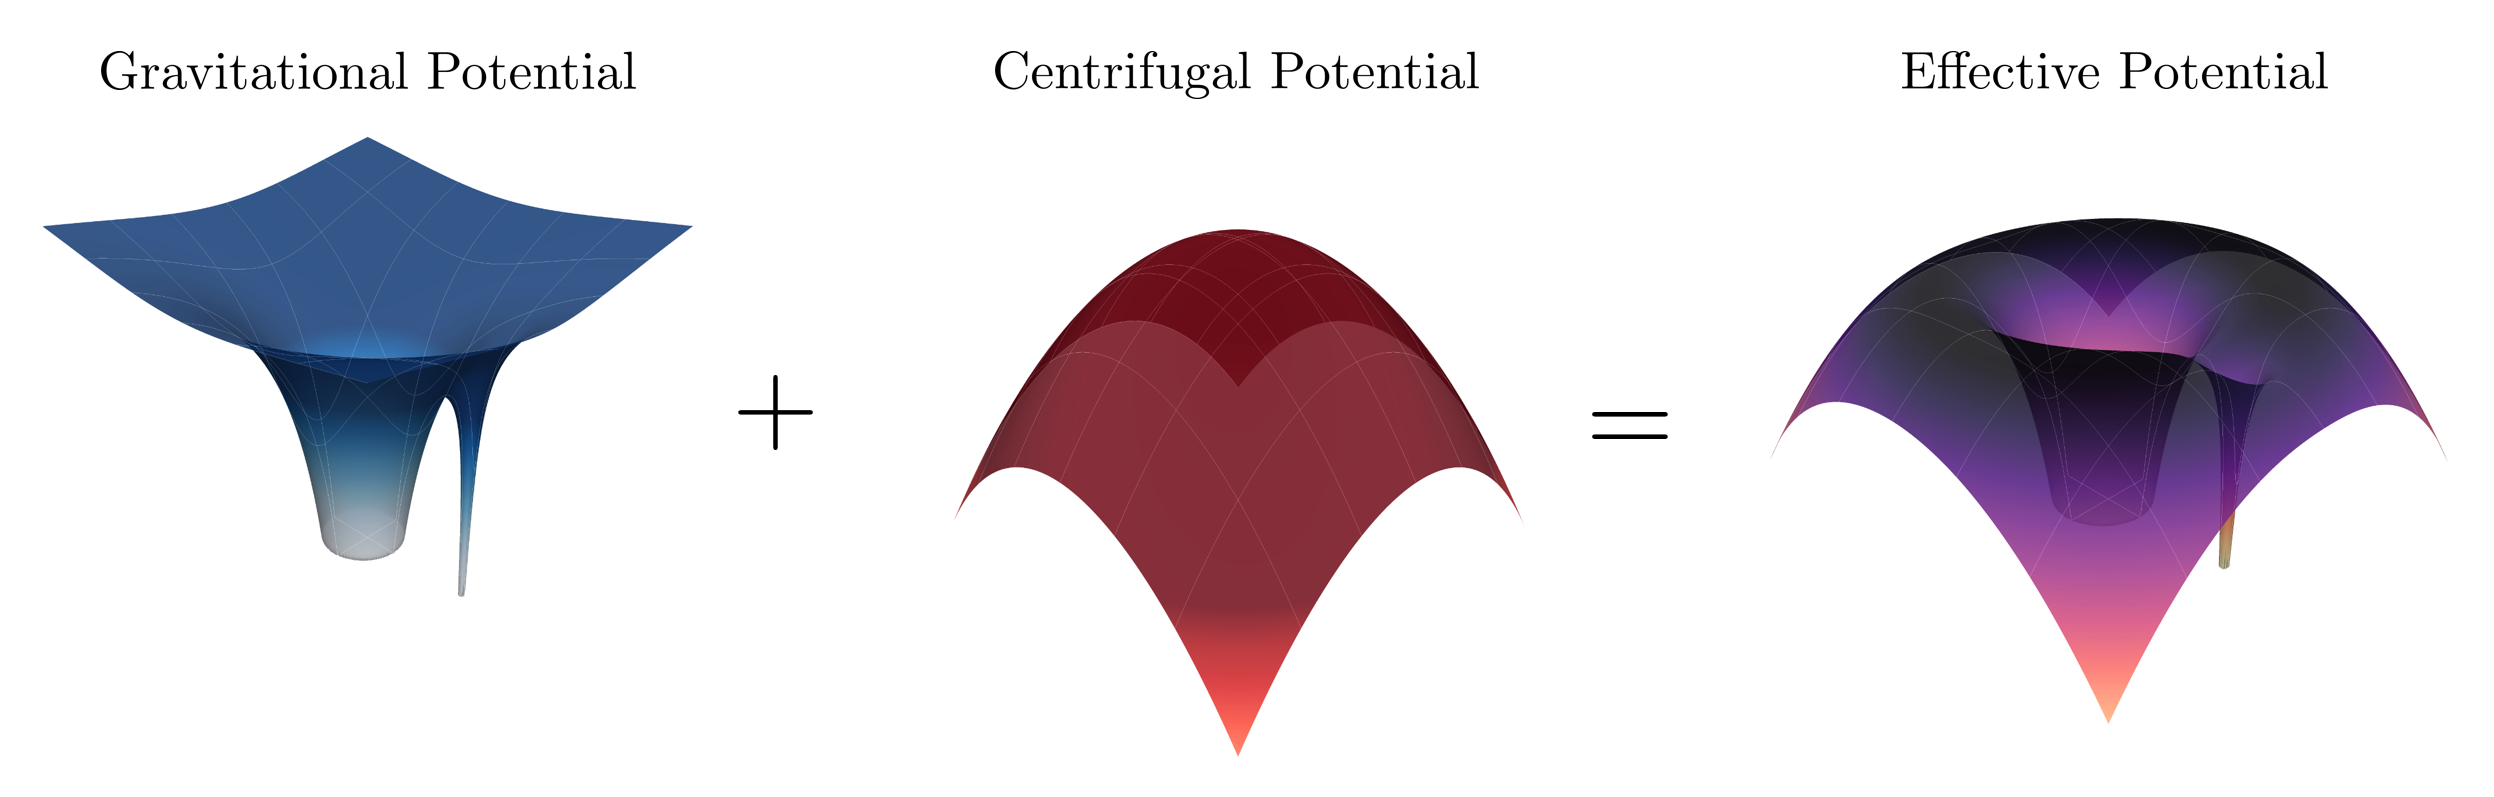
\includegraphics[width=\linewidth]{images/Potentials.png}
    \caption{Illustration of scalar potentials governing the CR3BP dynamics.}
    \label{fig:effective_potential}
\end{figure}

Since the system is closed, the total energy of the smallest body $m$ in the synodic frame is conserved. We identify the total energy as the sum of kinetic and potential energies. This quantity is the Hamiltonian of the system in \eqref{eq:cr3bp_acceleration}, written as
\begin{equation} \label{eq:hamiltonian_definition}
    H = \frac{1}{2}\|\boldsymbol{v}\|_2^2 + \tilde{U} = \frac{1}{2}\left(v_x^2 + v_y^2 +v_z^2\right) -\frac{1-\mu}{\rho_1} - \frac{\mu}{\rho_2} -\frac{1}{2}\left(x^2 + y^2\right).
\end{equation}
It is easy to show that the dynamics \eqref{eq:cr3bp_acceleration} can be rewritten in terms of the Hamiltonian as 
\begin{align*}
    \dot{\boldsymbol{r}} &= \nabla_{\boldsymbol{v}} H, \\
    \dot{\boldsymbol{v}} &= 
    \begin{pmatrix}
        0 & 2 & 0 \\
        -2 & 0 & 0 \\
        0 & 0 & 0
    \end{pmatrix}
    \nabla_{\boldsymbol{v}} H
    - \nabla_{\boldsymbol{r}} H,
\end{align*}
where the first term in the $\dot{\boldsymbol{v}}$ equation represents the Coriolis acceleration. We remark that this term can be eliminated by simply transforming to canonical coordinates; in these coordinates, the velocity $\boldsymbol{v}$ is replaced by canonical momentum $\boldsymbol{p}$, which, in the rotating frame, is given by $\boldsymbol{p} = (v_x -y, v_y+x, v_z)$. In $\boldsymbol{z} \coloneq(\boldsymbol{r}, \boldsymbol{p})$ coordinates, the system satisfies the Hamilton canonical equation
\begin{equation} \label{eq:hamilton_canonical_equation}
    \dot{\boldsymbol{z}} = \boldsymbol{J} \nabla H(\boldsymbol{z}), \qquad
    \boldsymbol{J} = \begin{pmatrix}
    0 & I \\
    - I & 0
    \end{pmatrix},
\end{equation}
where $\boldsymbol{J}$ is the canonical symplectic matrix. The CR3BP system is therefore Hamiltonian.


\clearpage

In the astrodynamics literature, the total energy of the CR3BP is often referred to in terms of the system's first integral of motion, the \emph{Jacobi integral} $C$, which can be written in terms of the Hamiltonian as
\begin{equation} \label{eq:jacobi_integral}
    C = -2H.
\end{equation}

The conservation of the Hamiltonian (and consequently the Jacobi integral) places strict topological bounds on the motion of the spacecraft. Because the kinetic energy must be a non-negative real value ($\frac{1}{2}\|\boldsymbol{v}\|_2^2 \ge 0$), the spacecraft is physically constrained to regions of space where its total energy is greater than or equal to the local effective potential:
\begin{equation*}
    C \leq 2\tilde{U}.
\end{equation*}
The boundaries of these allowed regions, defined by the condition where the kinetic energy drops exactly to zero ($C = 2\tilde{U}$), are known as the \emph{Zero Velocity Surfaces} (ZVS). In the planar case ($z=0$), these project as \emph{Zero Velocity Curves} (ZVC). The spatial volumes bounded by these surfaces are referred to as \emph{Hill's regions}. A spacecraft possessing a specific Hamiltonian cannot traverse the ZVS; it is strictly confined to the connected Hill's region in which it originated. These boundaries serve as hard reachability limits dictated by the combined gravitational and centrifugal landscapes, as visualized in \cref{fig:hills_regions}.

\begin{figure}[htbp]
    \centering

    \begin{subfigure}{0.4\textwidth}
        \centering
        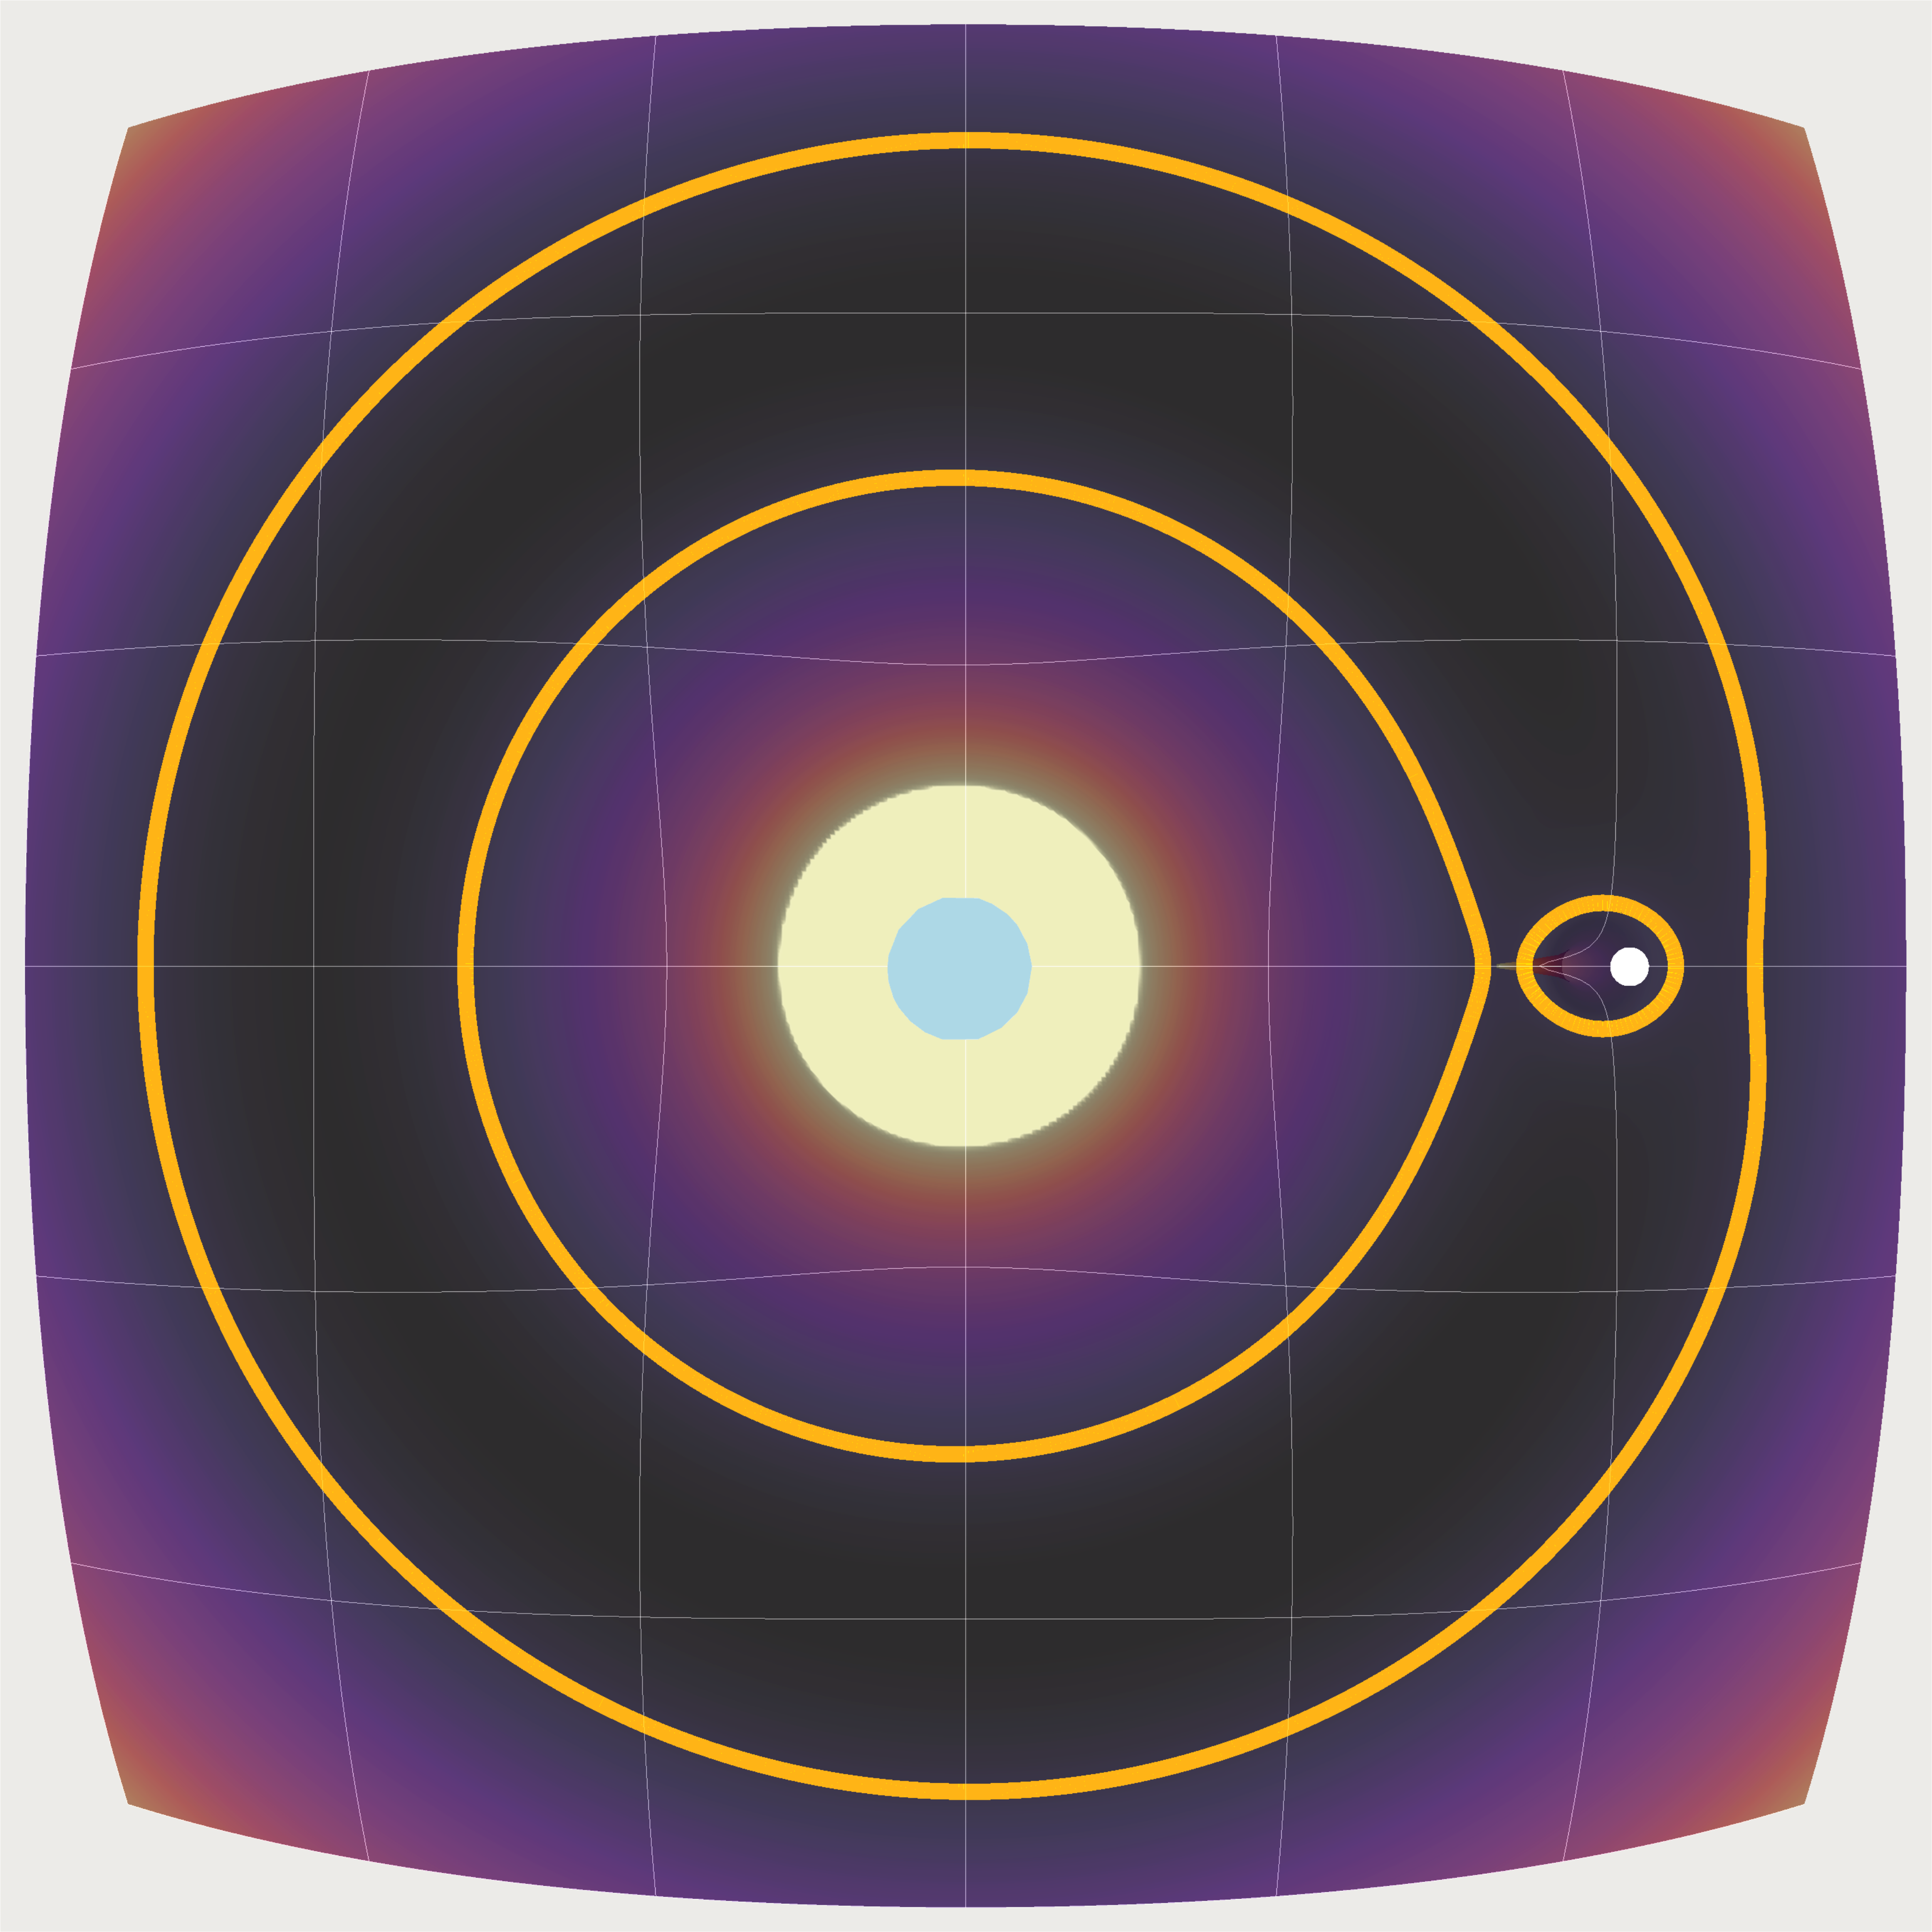
\includegraphics[width=\linewidth]{images/hill_curve_3.20.png}
        \caption{$C \in (C_1, C_2)$}
        \label{fig:hills_regions_c1c2}
    \end{subfigure}
    \hspace{1.5em}
    \begin{subfigure}{0.4\textwidth}
        \centering
        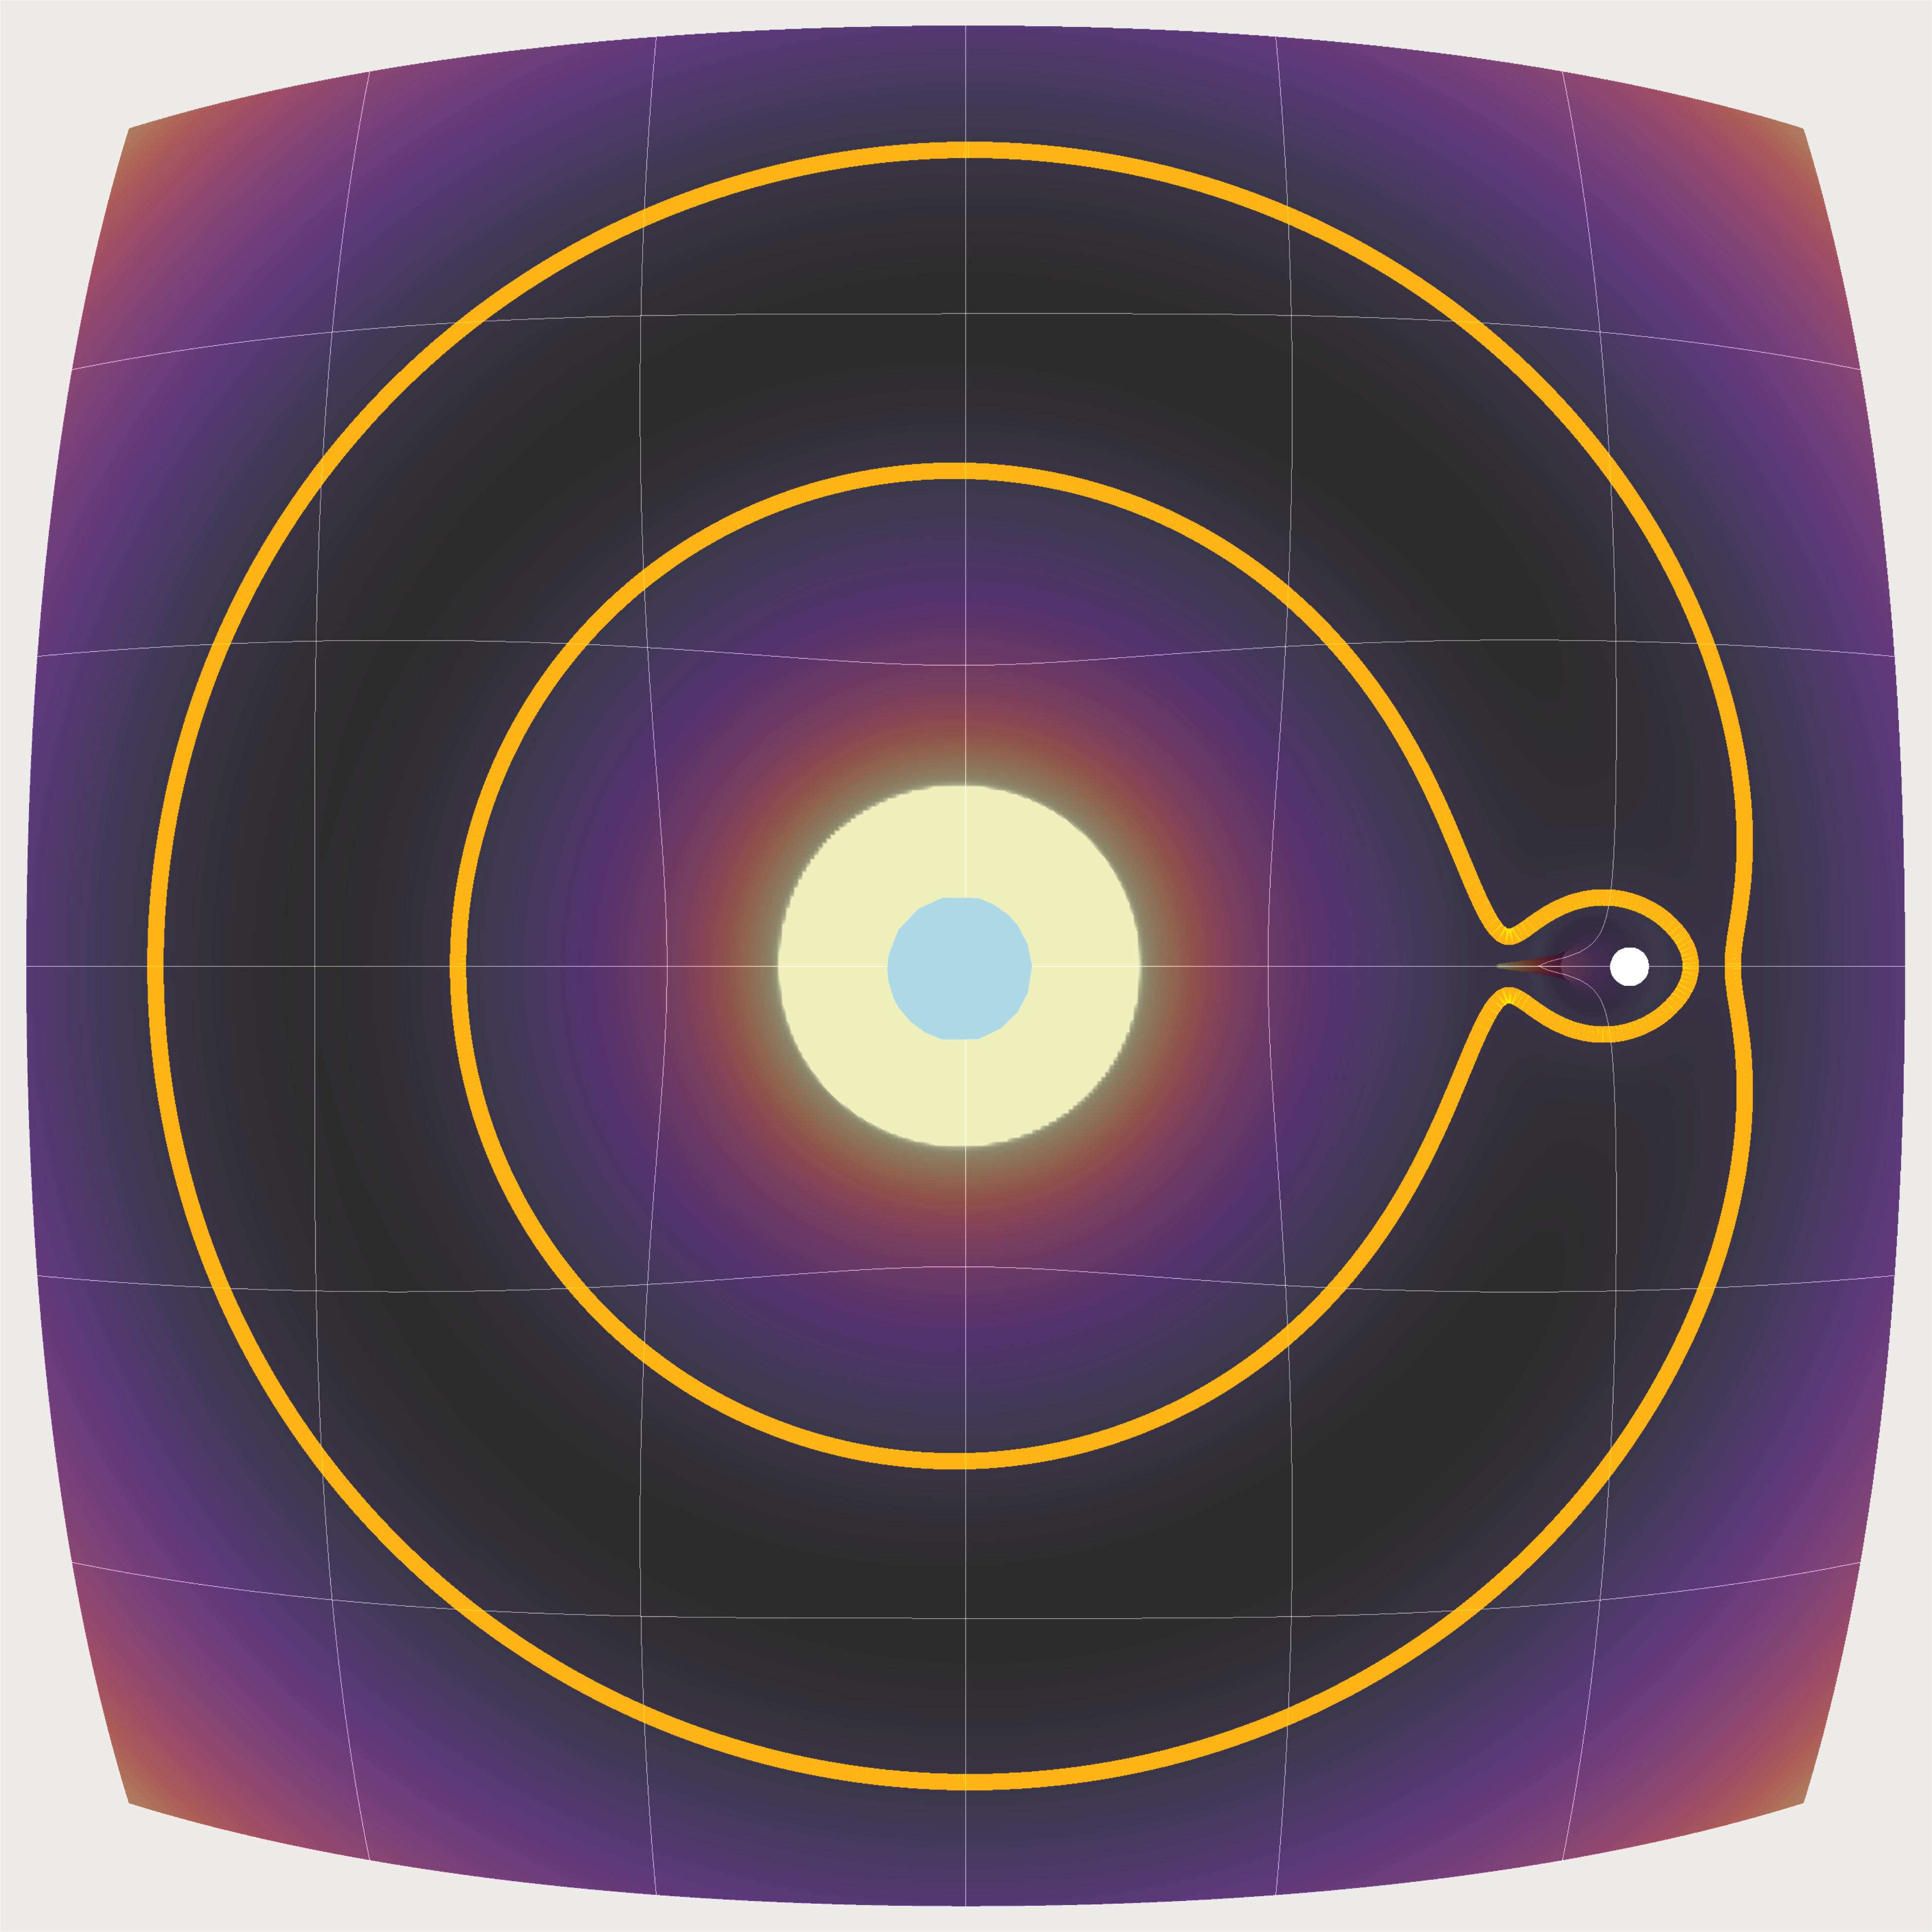
\includegraphics[width=\linewidth]{images/hill_curve_3.18.png}
        \caption{$C \in (C_2, C_3)$}
        \label{fig:hills_regions_c2c3}
    \end{subfigure}

    \vspace{0.5em}

    \begin{subfigure}{0.4\textwidth}
        \centering
        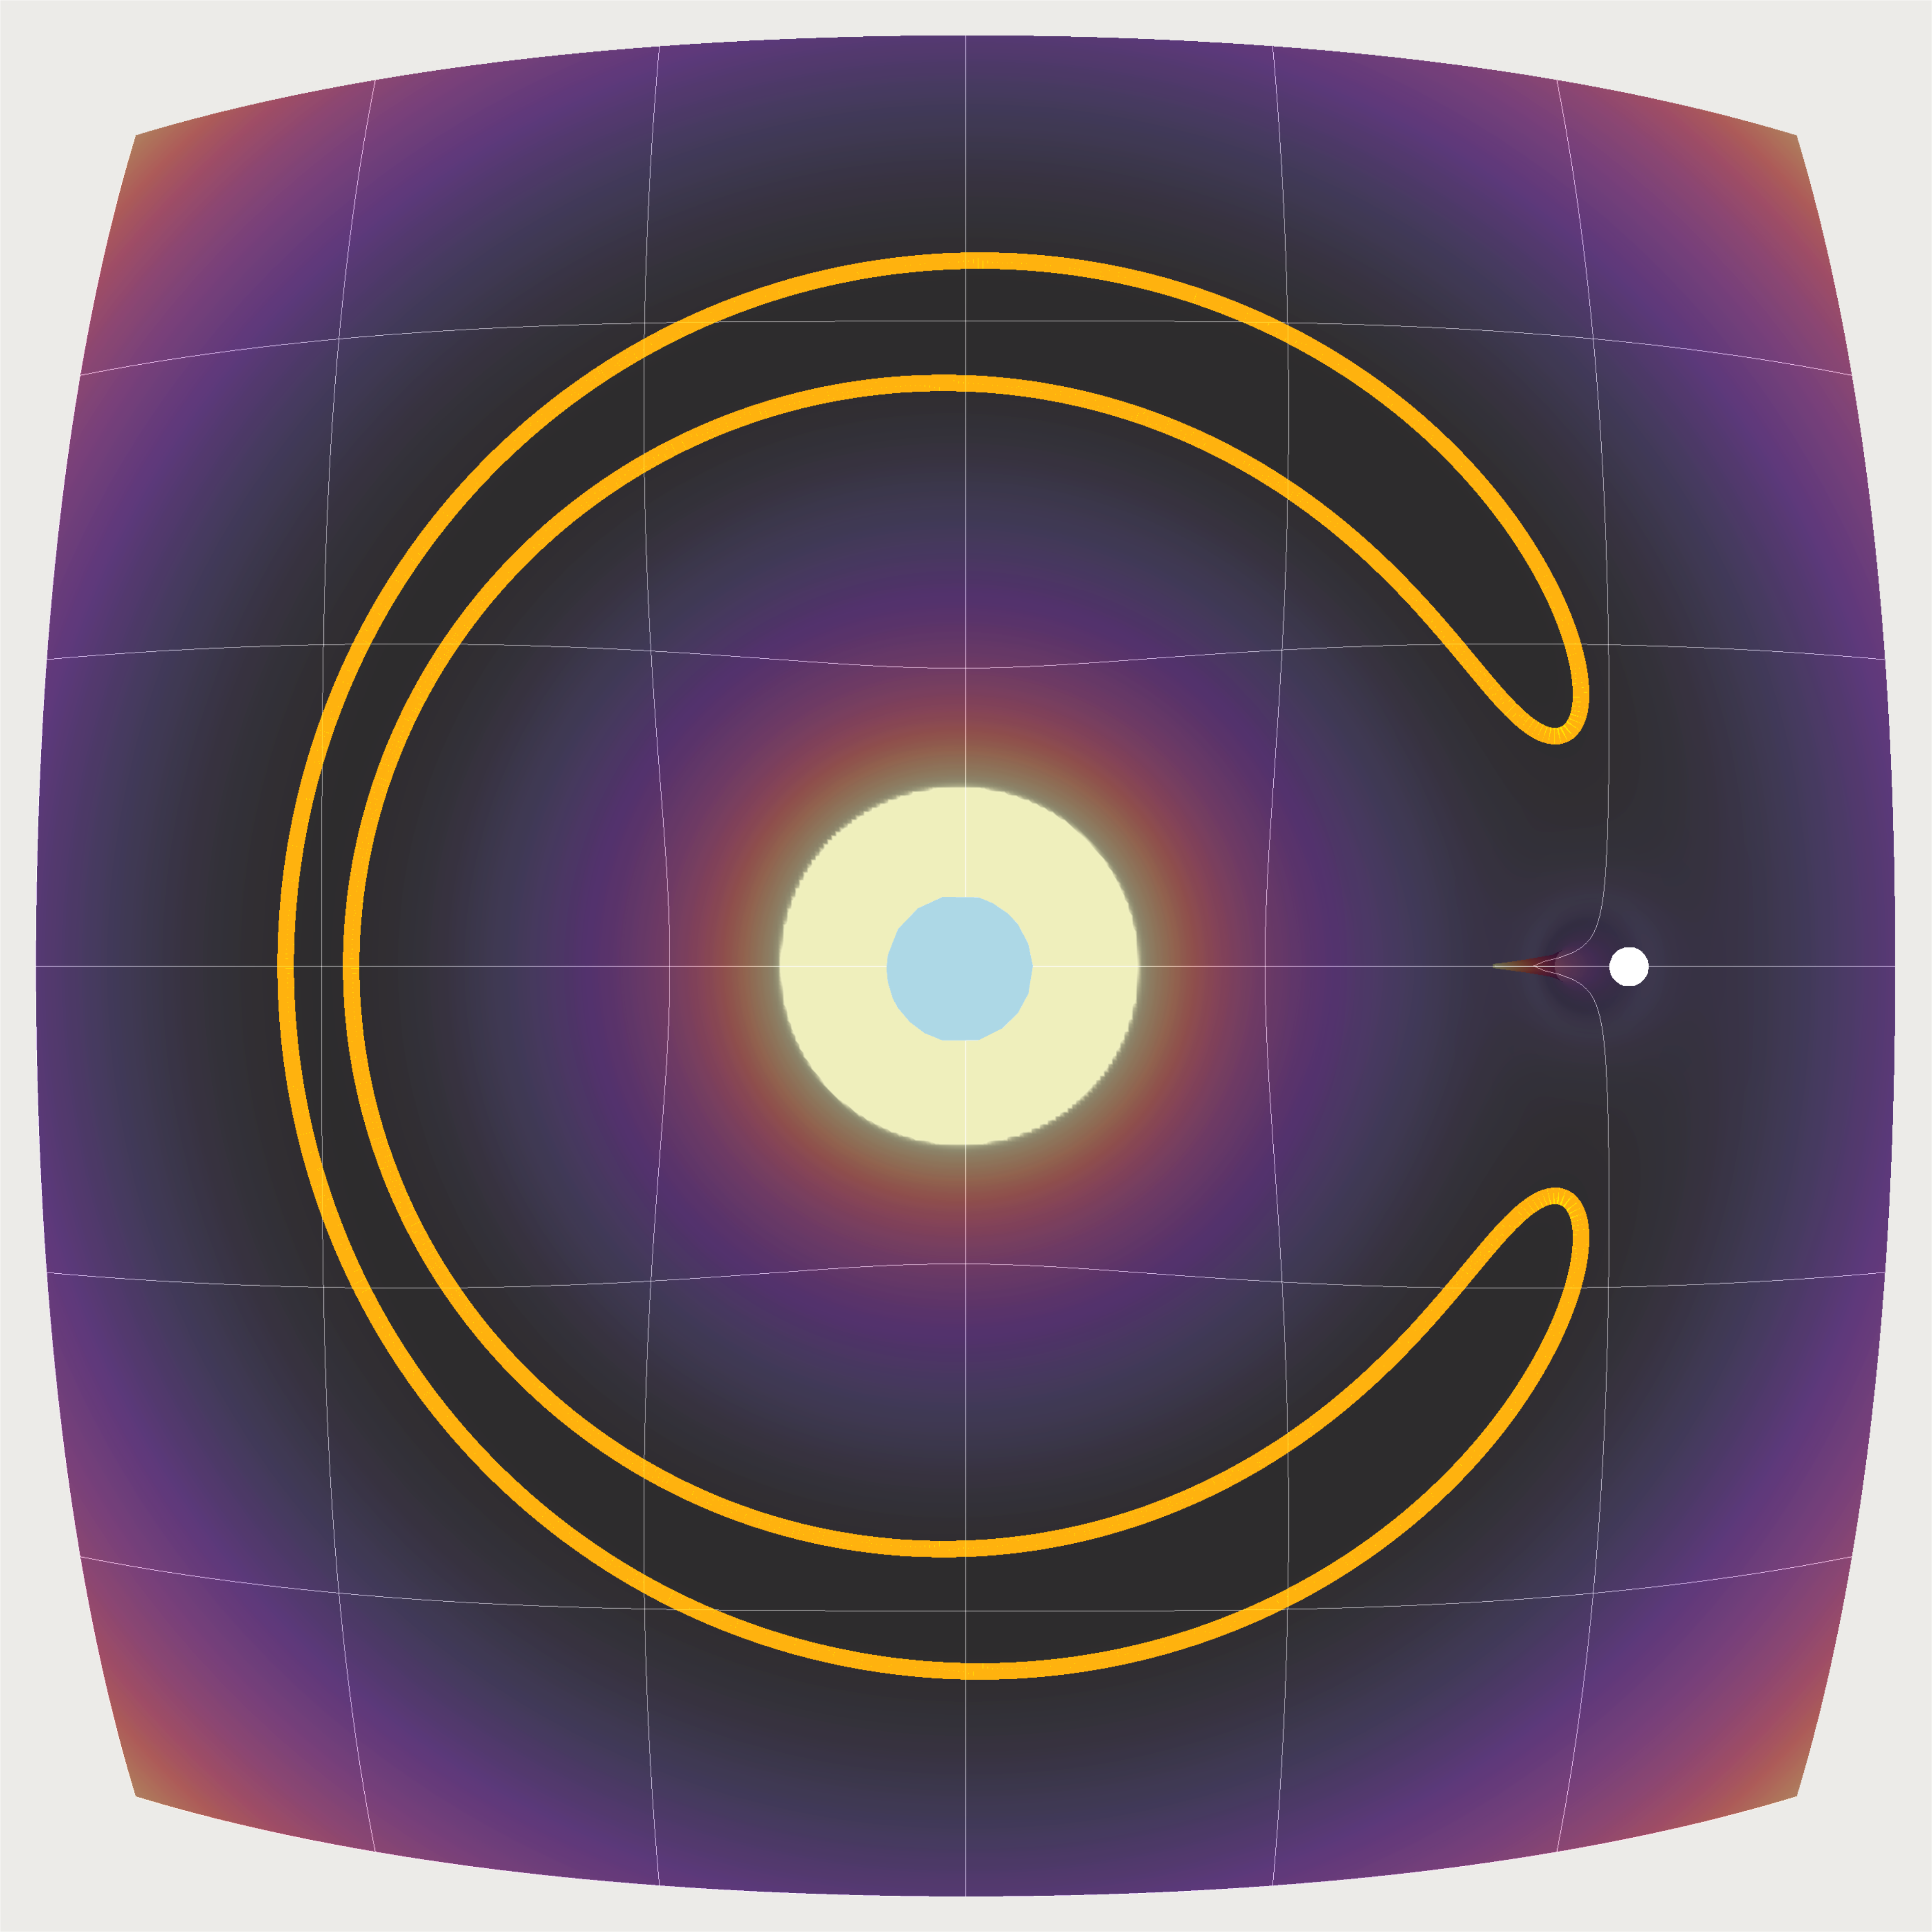
\includegraphics[width=\linewidth]{images/hill_curve_3.02.png}
        \caption{$C \in (C_3, C_4)$}
        \label{fig:hills_regions_c3c4}
    \end{subfigure}
    \hspace{1.5em}
    \begin{subfigure}{0.4\textwidth}
        \centering
        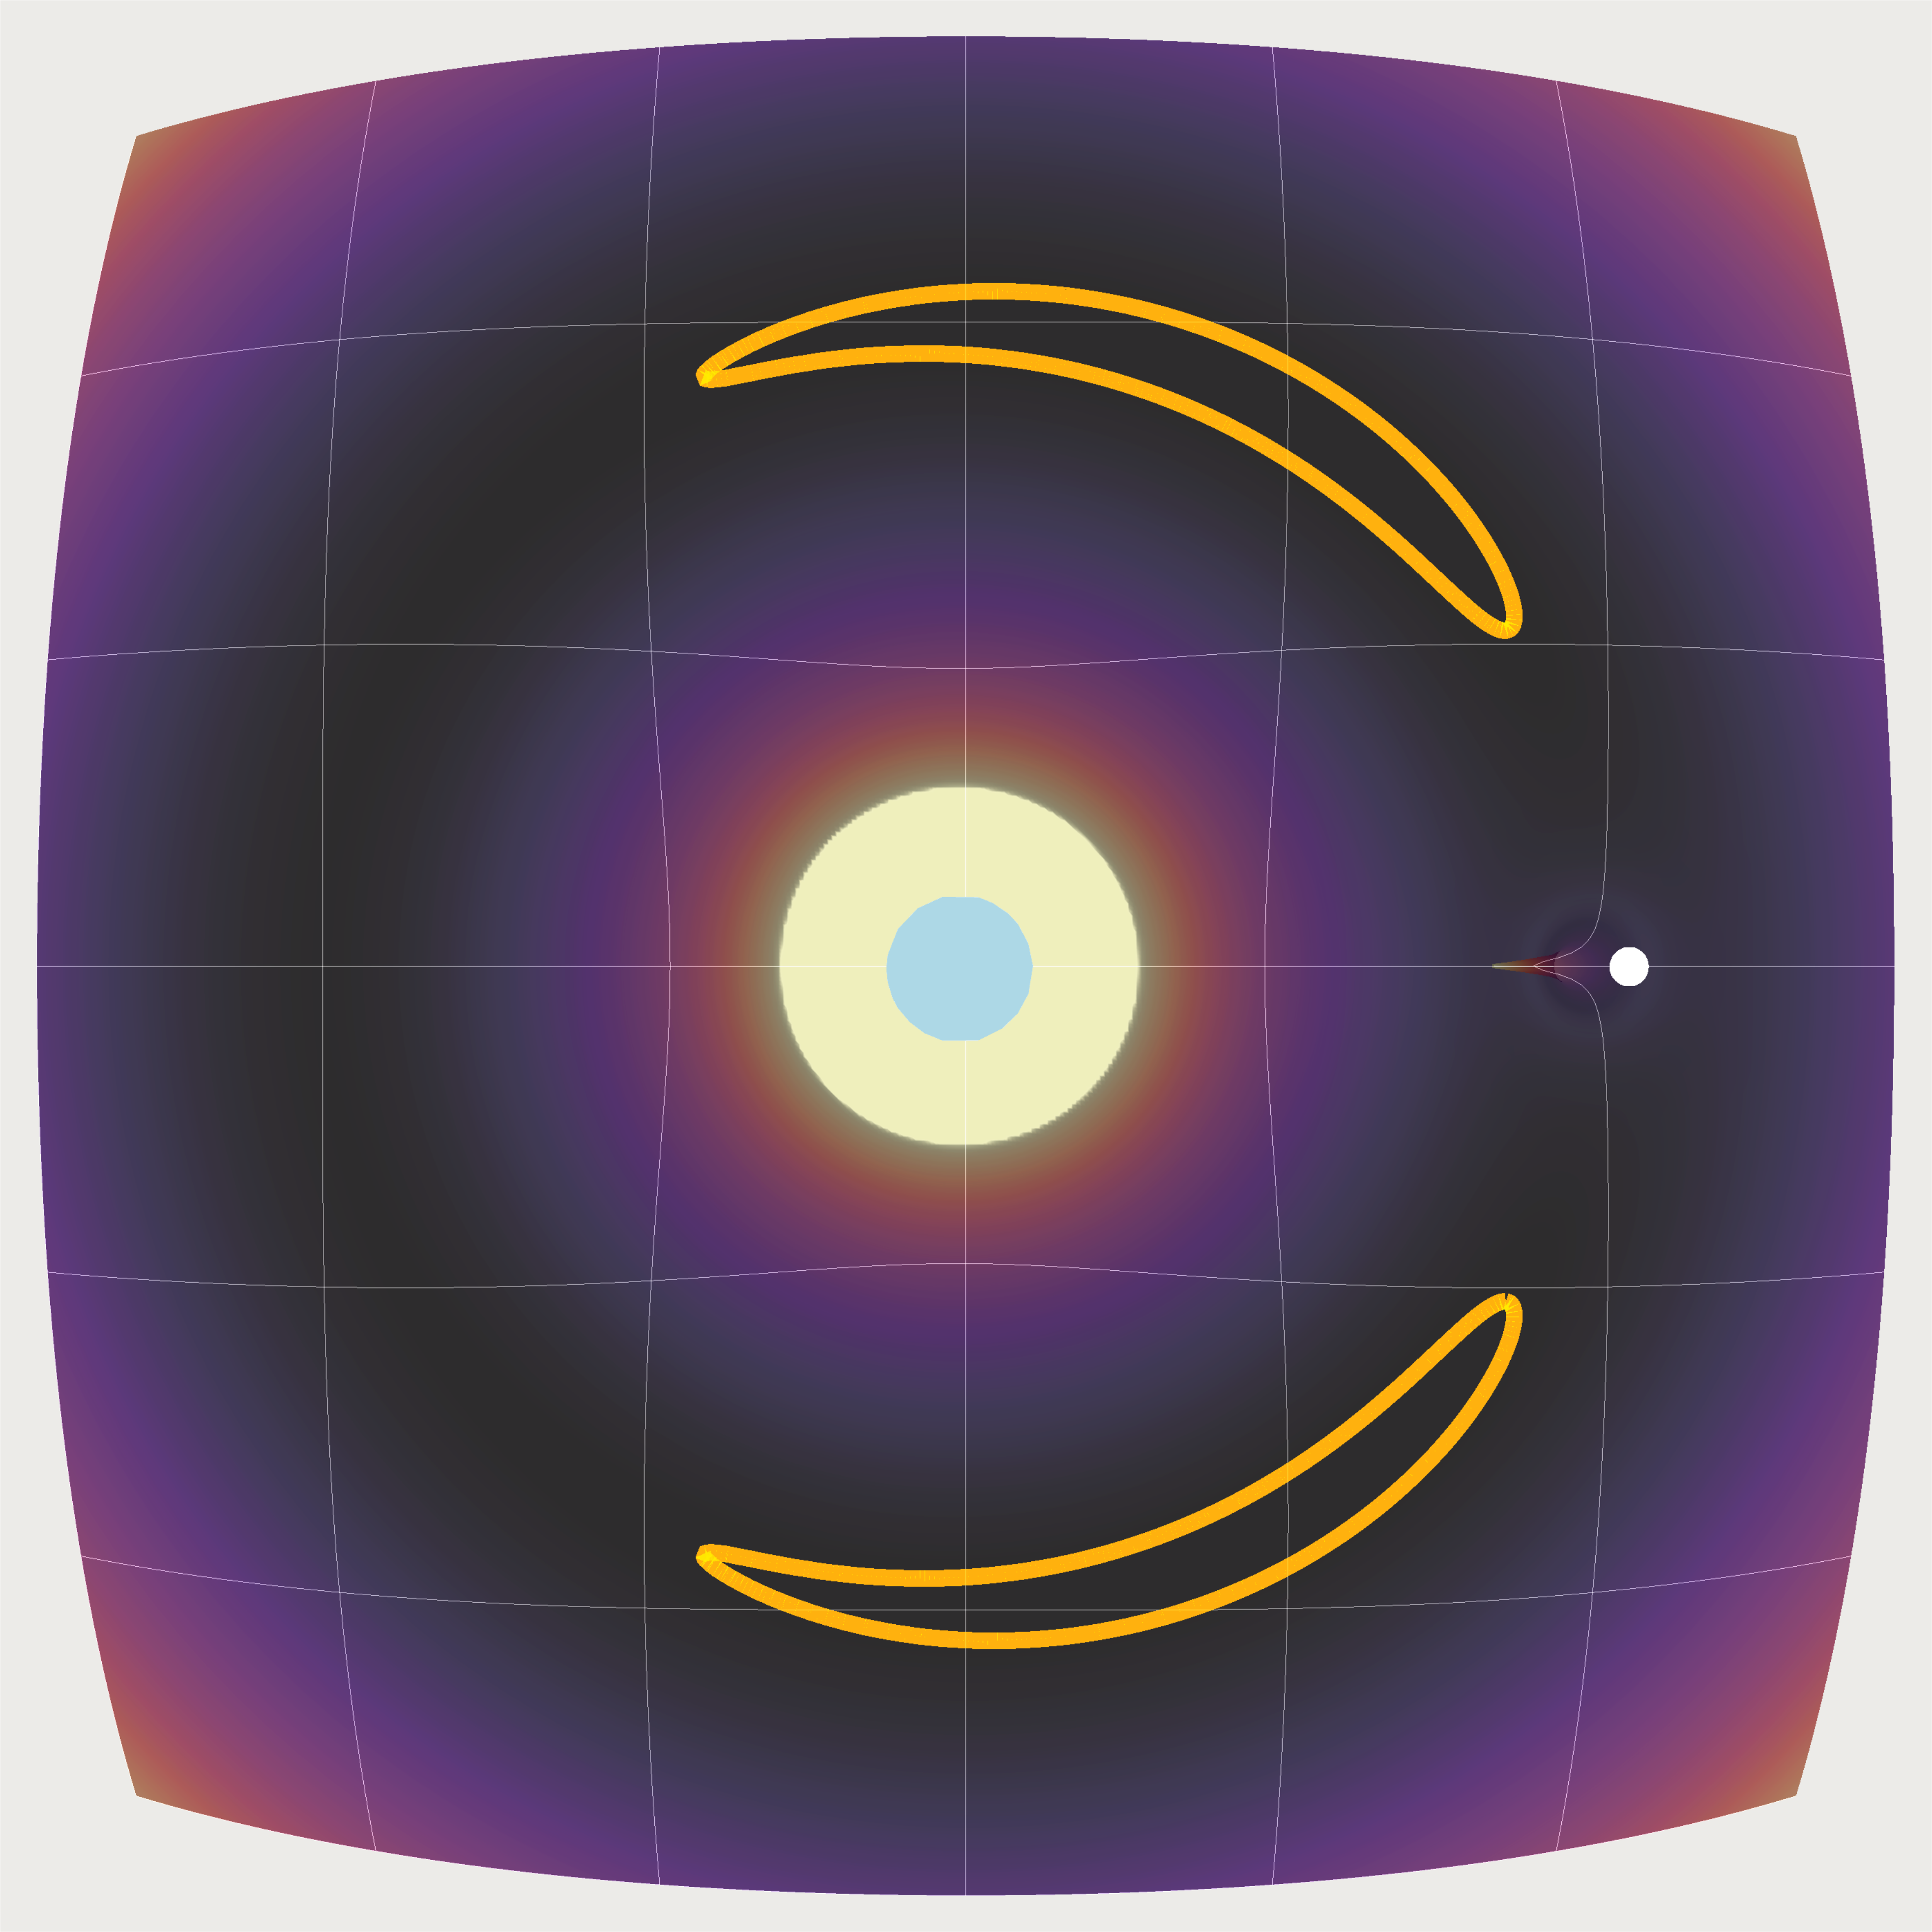
\includegraphics[width=\linewidth]{images/hill_curve_3.00.png}
        \caption{$C \in (C_4, C_5)$}
        \label{fig:hills_regions_c4c5}
    \end{subfigure}

    \caption{Hill's regions across Jacobi integral ranges.}
    \label{fig:hills_regions}
\end{figure}

\clearpage

\begin{figure}[htbp]
    \centering
    \begin{tikzpicture}
        \begin{axis}[
            axis equal image,
            hide axis,
            width=8cm, 
            height=9cm,
            clip=false,
            axis lines=middle,
            ticks=none
        ]
    
        % Masses m1 and m2
        \addplot[mark=*, mark size=6pt, only marks, color=brown!90!red] coordinates {(-0.13, 0)}; 
        \node at (axis cs:-0.13, 0.06) {$m_1$}; 
        \node at (axis cs:-0.15, -0.07) {$(-\mu, 0, 0)$}; 
        \addplot[mark=*, mark size=4pt, only marks, color=brown!90!red] coordinates {(0.41, 0)}; 
        \node at (axis cs:0.41, 0.05) {$m_2$}; 
        \node at (axis cs:0.46, -0.175) {$(1 - \mu, 0, 0)$}; 
        \draw[] (axis cs:0.46, -0.15) -- (axis cs:0.42, -0.03);
    
        % Adding nodes L4 and L5
        \addplot[mark=x, mark size=3pt, thick, only marks, color=blue] coordinates {(0.14, 0.468)}; 
        \node at (axis cs:0.2, 0.468) {$\mathcal{L}_4$};
        
        \addplot[mark=x, mark size=3pt, thick, only marks, color=blue] coordinates {(0.14, -0.468)}; 
        \node at (axis cs:0.2, -0.468) {$\mathcal{L}_5$};
    
        % Adding nodes L1,L2 and L3
        \addplot[mark=x, mark size=3pt, thick, only marks, color=blue] coordinates {(0.27, 0)}; 
        \node at (axis cs:0.27, 0.05) {$\mathcal{L}_1$};
        
        \addplot[mark=x, mark size=3pt, thick, only marks, color=blue] coordinates {(0.55, 0)}; 
        \node at (axis cs:0.55, 0.05) {$\mathcal{L}_2$};
    
        \addplot[mark=x, mark size=3pt, thick, only marks, color=blue] coordinates {(-0.5, 0)}; 
        \node at (axis cs:-0.5, 0.05) {$\mathcal{L}_3$};
        
        % Point P
        \addplot[mark=*, mark size=1.5pt, only marks, color=black] coordinates {(0.25, 0.275)}; 
        \node at (axis cs:0.25, 0.315) {$P$}; 
        \node at (axis cs:0.25, 0.235) {$(x, y, z)$}; 
    
        % Axes
        \draw[->, >=stealth, thick] (-0.55, 0) -- (0.8, 0) node[ below] {$x$}; 
        \draw[->, >=stealth, thick] (0, -0.5) -- (0, 0.6) node[left] {$y$}; 
        %\draw[->, >=stealth, thick] ($(0.07*1.4142, 0.07*1.4142)$) -- ($(-0.07*1.4142, -0.07*1.4142)$) node[below right] {$z$}; 
    
        % Setting axis limits
        \path (axis cs:-0.125,-0.1) rectangle (axis cs:0.6,0.5); 
    
        \end{axis}
    \end{tikzpicture}
    \caption{Caption}
    \label{fig:placeholder}
\end{figure}



\newpage %temporarily

\section{Computing Periodic Orbits} 
\label{sec:ComputingPeriodicOrbits}

\subsection{Families of Periodic Orbits}
The CR3BP admits infinitely many periodic orbits \cite{Poincare_1957}.
Many of these orbit families have been studied extensively and several have found practical applications in space mission design. 
In this work, we restrict our analysis to planar periodic orbits and illustrate how they can be computed numerically using differential correction. 
An initial condition $\boldsymbol{x}_0$ lies on a periodic orbit if there exists a time $T>0$ such that
\begin{equation*}
    \boldsymbol{\phi}(T,\boldsymbol{x}_0) =\boldsymbol{x}_0.
\end{equation*}
The smallest positive value of $T$ is called the period of the orbit.

\begin{figure*}[t!]
  \centering
  \begin{subfigure}[b]{0.32\linewidth}
    \centering
    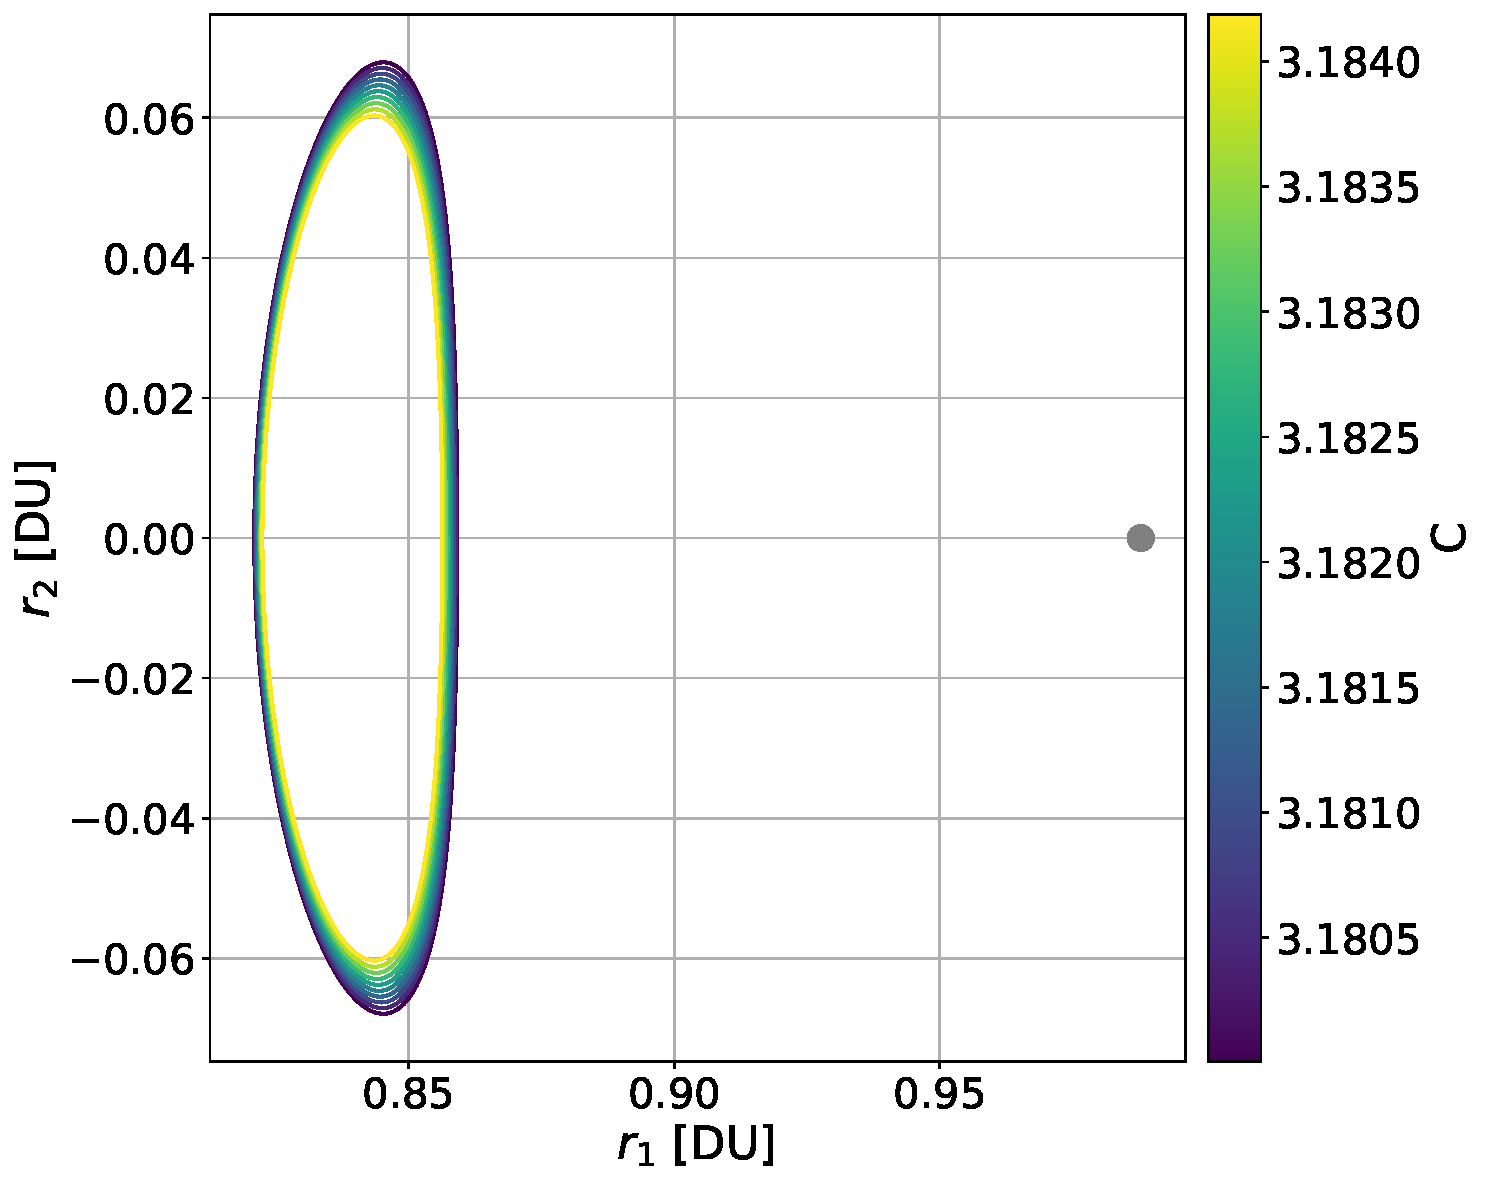
\includegraphics[width=\linewidth]{images/lyapunov_step20_E-1.584--1.586.pdf}
    \caption{Lyapunov}
    \label{fig:sub_a}
  \end{subfigure}
  \hfill
  \begin{subfigure}[b]{0.32\textwidth}
    \centering
    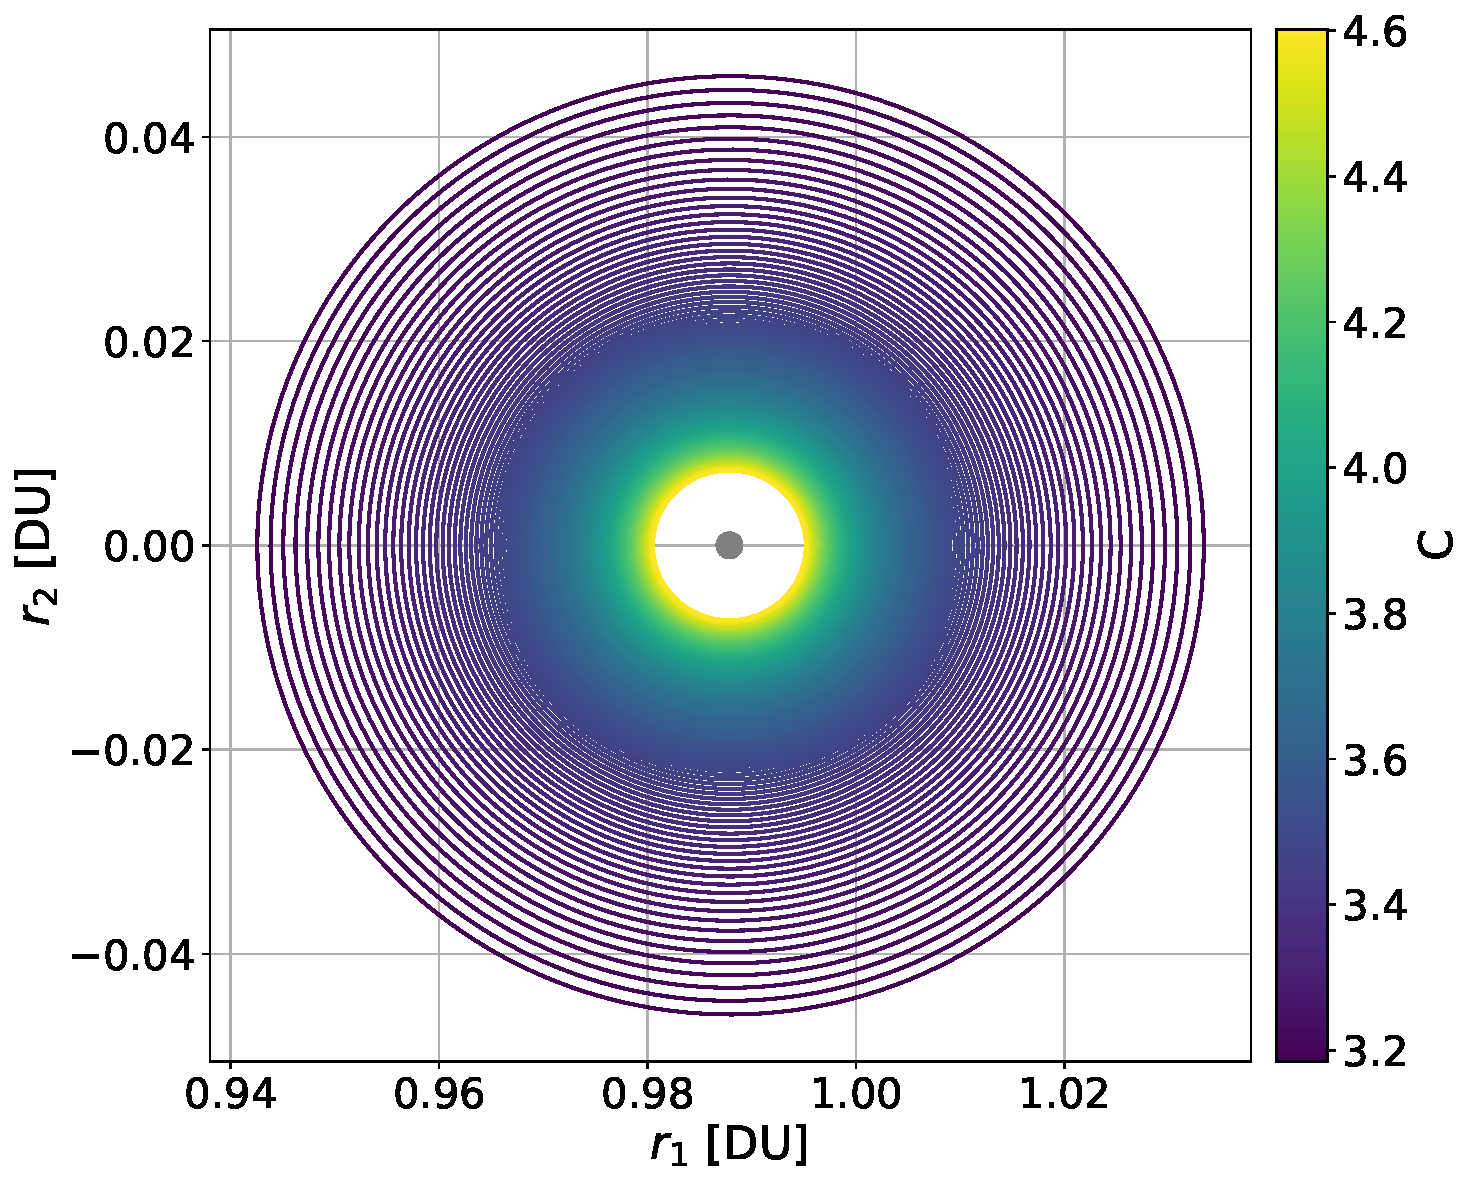
\includegraphics[width=\linewidth]{images/dros_step15_jacobimin3.172.pdf}
    \caption{DRO}
    \label{fig:sub_b}
  \end{subfigure}
  \hfill
  \begin{subfigure}[b]{0.32\textwidth}
    \centering
    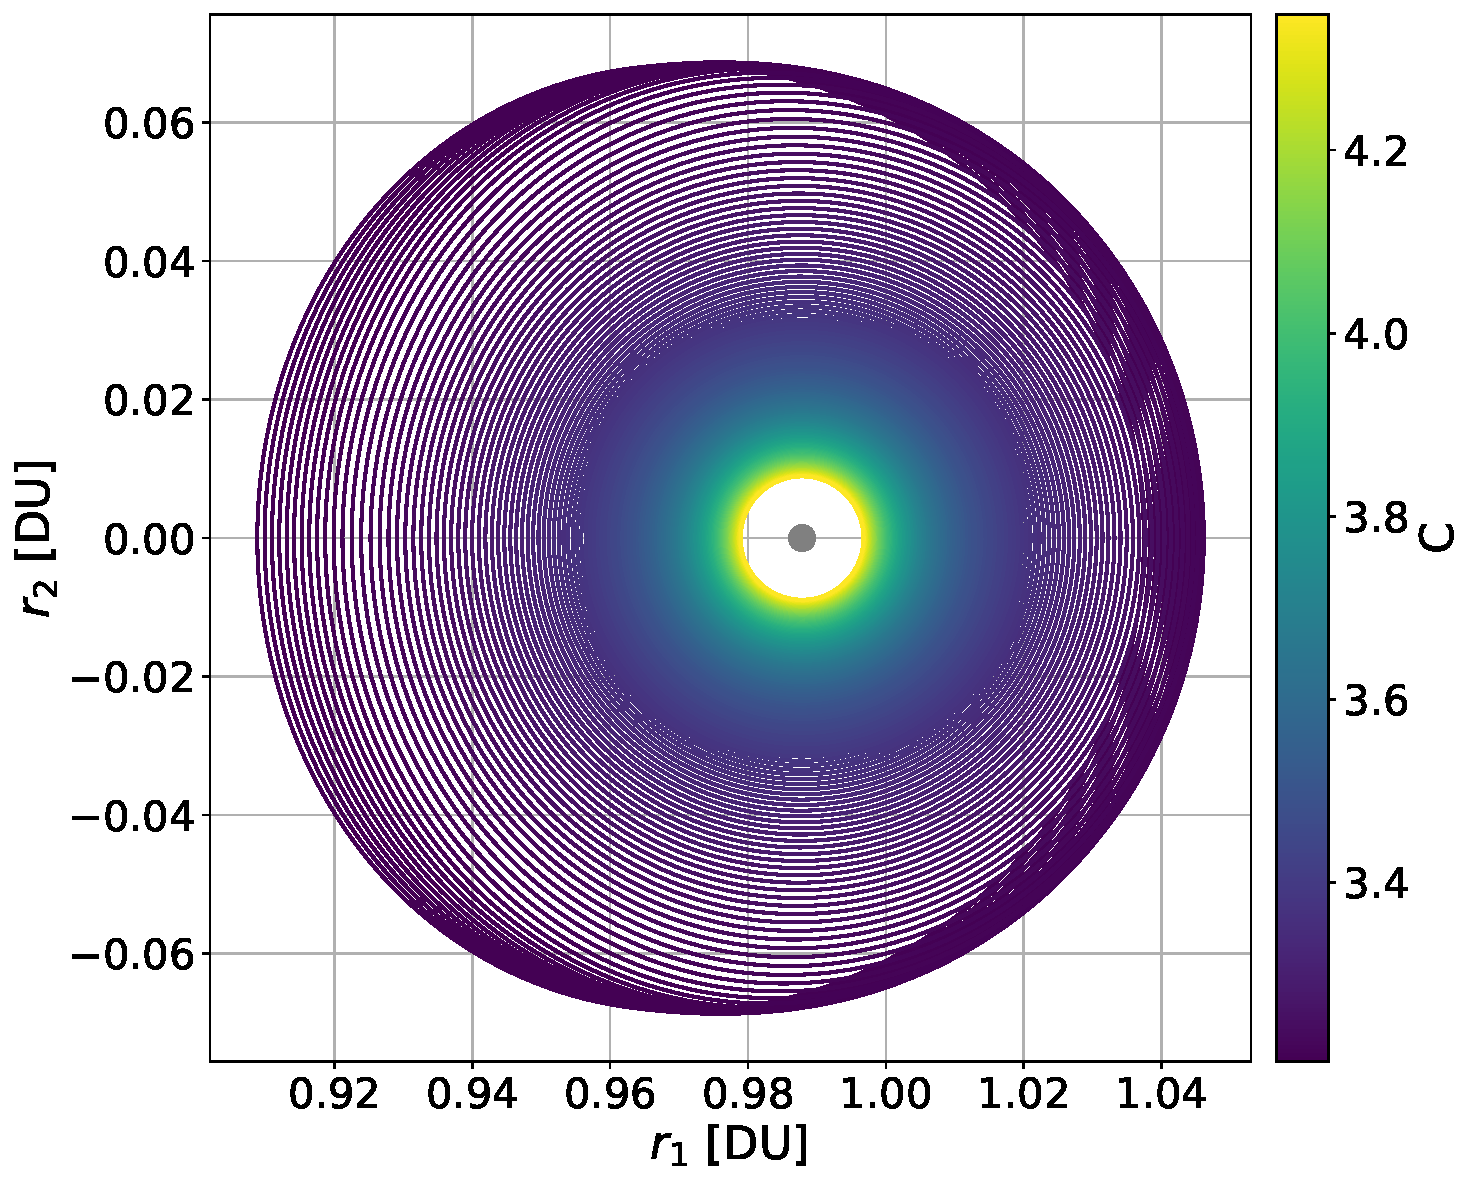
\includegraphics[width=\linewidth]{images/dpos_step15_jacobimin3.172.pdf}
    \caption{DPO}
    \label{fig:sub_c}
  \end{subfigure}
  \caption{Examples of different families of orbits in the lunar regime, shown in the $x,y$ plane of the CR3BP. Colours indicate the Jacobi constant for each orbit.}
  \label{fig:lunar_orbits}
\end{figure*}
Starting from an initial guess for the state $\boldsymbol{x}_0$, periodic orbits can be computed using a differential correction algorithm. \cref{fig:lunar_orbits} shows representative planar periodic orbits in the lunar region. 
These include Moon-centred orbit families, such as distant retrograde orbits (DROs) and distant prograde orbits (DPOs), as well as equilibrium-point-centred families, such as Lyapunov orbits.
\begin{figure*}[b!]
  \centering
  \begin{subfigure}[b]{0.32\linewidth}
    \centering
    \includegraphics[width=\linewidth]{images/resonant_7.0_1.0_retro_False_step20_jacobimin3.172.png}
    \caption{7:1 Prograde}
    \label{fig:suba}
  \end{subfigure}
  \hfill
  \begin{subfigure}[b]{0.32\textwidth}
    \centering
    \includegraphics[width=\linewidth]{images/resonant_9.0_2.0_retro_False_step20_jacobimin3.172.png}
    \caption{9:2 Prograde}
    \label{fig:subb}
  \end{subfigure}
  \hfill
  \begin{subfigure}[b]{0.32\textwidth}
    \centering
    \includegraphics[width=\linewidth]{images/resonant_10.0_3.0_retro_False_step20_jacobimin3.172.png}
    \caption{10:3 Retrograde}
    \label{fig:subc}
  \end{subfigure}
  \caption{Examples of different resonant orbit families, shown in the $x,y$ plane of the CR3BP. Colours indicate the Jacobi constant for each orbit.}
  \label{fig:resonant_orbit_families}
\end{figure*}

Another important class of planar periodic orbits in the CR3BP is given by resonant orbits. 
A $p:q$ resonant orbit completes $p$ revolutions around the Earth in the same time that the Moon completes $q$ revolutions around the Earth, where $p$ and $q$ are integers. 
Depending on the direction of motion around the Earth, resonant orbits can be either prograde or retrograde. 
Examples of several resonant orbit families are shown in \cref{fig:resonant_orbit_families}.
\subsection{Differential Correction}
Differential correction is a Newton-type method for refining an approximate trajectory until it satisfies a prescribed set of boundary conditions. 
Many trajectory-design problems can be formulated as finding a vector of free variables $\boldsymbol{X}$ such that
\[
    \boldsymbol{F}(\boldsymbol{X}) = \boldsymbol{0},
\]
where $\boldsymbol{F}$ is a constraint vector measuring the violation of the desired boundary conditions.
For example, in the simplest periodic-orbit problem, the free variables may be the initial condition $\boldsymbol{x}_0$ and the period $T$, and the constraint is
\[
    \boldsymbol{F}(\boldsymbol{x}_0,T)
    =
    \boldsymbol{\phi}(T,\boldsymbol{x}_0)-\boldsymbol{x}_0.
\]
A periodic orbit is obtained when this residual vanishes.

Starting from an initial guess $\boldsymbol{X}^{(k)}$, differential correction linearizes the constraint vector as
\[
    \boldsymbol{F}(\boldsymbol{X}^{(k)}+\delta\boldsymbol{X})
    \approx
    \boldsymbol{F}(\boldsymbol{X}^{(k)})
    +
    D\boldsymbol{F}(\boldsymbol{X}^{(k)})\delta\boldsymbol{X},
\]
where $D\boldsymbol{F}(\boldsymbol{X}^{(k)})$ is the Jacobian of the constraints with respect to the free variables. 
The correction $\delta\boldsymbol{X}$ is chosen so that the linearized residual is zero:
\begin{equation}
\label{eq: differential correction}
    D\boldsymbol{F}(\boldsymbol{X}^{(k)})\delta\boldsymbol{X}
    =
    -\boldsymbol{F}(\boldsymbol{X}^{(k)}).
\end{equation}
The free variables are then updated according to
\begin{equation}
    \label{eq: DC Step}
    \boldsymbol{X}^{(k+1)}
    =
    \boldsymbol{X}^{(k)}
    +
    \delta\boldsymbol{X}.
\end{equation}
This process is repeated until the constraint residual satisfies
\[
    \left\|\boldsymbol{F}(\boldsymbol{X}^{(k)})\right\| < \varepsilon,
\]
for a prescribed tolerance $\varepsilon$.

In trajectory-design applications, the Jacobian $D\boldsymbol{F}$ is obtained from sensitivities of the flow map with respect to the free variables. 
In particular, the sensitivity of a state at time $t$ with respect to the initial state is given by the state transition matrix (STM)
\[
    \boldsymbol{\Phi}(t,\boldsymbol{x}_0)
    =
    \frac{\partial \boldsymbol{\phi}(t,\boldsymbol{x}_0)}
    {\partial \boldsymbol{x}_0}.
\]
The STM is computed by integrating the variational equations along the current trajectory,
\begin{equation} \label{eq: STM}
    \dot{\boldsymbol{\Phi}}(t)
    =
    D\boldsymbol{f}(\boldsymbol{x}(t))\boldsymbol{\Phi}(t),
    \qquad
    \boldsymbol{\Phi}(0)=I.
\end{equation}

For the planar CR3BP, the matrix $D\boldsymbol{f}$ is given by 
\begin{equation}
    D\boldsymbol{f}(\boldsymbol{x})
    =
    \begin{pmatrix}
    0 & 0 & 1 & 0 \\
    0 & 0 & 0 & 1 \\
    \dfrac{\partial g_x}{\partial x} & \dfrac{\partial g_x}{\partial y} & 0 & 2 \\
    \dfrac{\partial g_y}{\partial x} & \dfrac{\partial g_y}{\partial y} & -2 & 0
    \end{pmatrix},
\end{equation}
where
\begin{align}
    \dfrac{\partial g_x}{\partial x} 
    &= 1 - (1 - \mu) \left( \frac{1}{\rho_1^3} - 3 \frac{(x + \mu)^2}{\rho_1^5} \right)
         - \mu \left( \frac{1}{\rho_2^3} - 3 \frac{(x - 1 + \mu)^2}{\rho_2^5} \right), \\
    \dfrac{\partial g_y}{\partial y} 
    &= 1 - (1 - \mu) \left( \frac{1}{\rho_1^3} - 3 \frac{y^2}{\rho_1^5} \right)
         - \mu \left( \frac{1}{\rho_2^3} - 3 \frac{y^2}{\rho_2^5} \right), \\
    \dfrac{\partial g_x}{\partial y} 
    &= \dfrac{\partial g_y}{\partial x} 
    = 3(1-\mu)(x+\mu)\frac{y}{\rho_1^5}
      + 3\mu(x-1+\mu)\frac{y}{\rho_2^5}.
\end{align}
Thus, each differential-correction iteration requires integrating both the equations of motion and the associated variational equations.





\subsection{Computation of Planar Resonant Orbits} \label{subsec: computationOfPlanarResonantOrbits}

Since resonant orbits form one of the largest families of periodic orbits in the planar CR3BP, we describe their computation using differential correction in more detail. 
Due to the symmetries of the planar CR3BP, resonant orbits can be initialized at a crossing of the $x$-axis with $v_x=0$. 
This crossing point is used as the initial state on the orbit and has the form
\begin{equation*}
    \boldsymbol{x}_0 =
    \begin{pmatrix}
        x_0 \\
        0 \\
        0 \\
        v_{y,0}
    \end{pmatrix}.
\end{equation*}
Each family of resonant orbits exists over a range of $x_0$ values. 
To compute a specific member of such a family, $x_0$ is fixed, and the differential correction problem reduces to solving for the corresponding initial velocity $v_{y,0}$ and orbit period $T$.

To improve numerical stability, the periodicity condition is imposed using the symmetry of planar CR3BP orbits. 
Rather than correcting the trajectory over the full period, the initial condition is propagated for a half-period $T/2$, and the trajectory is required to reach the $x$-axis orthogonally. 
Therefore, the free-variable vector in the differential correction algorithm is
\begin{equation*}
    \boldsymbol{X}
    =
    \begin{pmatrix}
        v_{y,0} \\
        T/2
    \end{pmatrix}.
\end{equation*}
Using a single-shooting transcription, the initial condition is propagated to
\begin{equation*}
    \boldsymbol{x}_f
    =
    \boldsymbol{\phi}(T/2,\boldsymbol{x}_0)
    =
    \begin{pmatrix}
        x(T/2) \\
        y(T/2) \\
        v_x(T/2) \\
        v_y(T/2)
    \end{pmatrix}.
\end{equation*}
The half-period symmetry conditions are enforced through the differential-correction constraint vector
\begin{equation*}
    \boldsymbol{F}(\boldsymbol{X})
    =
    \begin{pmatrix}
        y(T/2) \\
        v_x(T/2)
    \end{pmatrix}
    =
    \boldsymbol{0}.
\end{equation*}
If these constraints are satisfied, the trajectory crosses the $x$-axis orthogonally after half a period, and the symmetry of the planar CR3BP can be used to recover the full periodic orbit.

The Jacobian required for the differential correction step in \cref{eq: differential correction} contains the sensitivities of the final values $y(T/2)$ and $v_x(T/2)$ with respect to the initial velocity $v_{y,0}$ and the propagation time $T/2$:
\begin{equation*}
    D\boldsymbol{F}(\boldsymbol{X})
    =
    \begin{pmatrix}
        \dfrac{\partial y_f}{\partial v_{y,0}}
        &
        \dfrac{\partial y_f}{\partial (T/2)}
        \\[1.2em]
        \dfrac{\partial v_{x,f}}{\partial v_{y,0}}
        &
        \dfrac{\partial v_{x,f}}{\partial (T/2)}
    \end{pmatrix}.
\end{equation*}
The first column is obtained from the entries in rows $2$ and $3$ of column $4$ of the state transition matrix
\begin{equation*}
    \boldsymbol{\Phi}(T/2,\boldsymbol{x}_0)
    =
    \frac{\partial \boldsymbol{\phi}(T/2,\boldsymbol{x}_0)}
    {\partial \boldsymbol{x}_0},
\end{equation*}
where the state ordering is $\boldsymbol{x}=(x,y,v_x,v_y)$. 
The second column is given by elements $2$ and $3$ of the vector field evaluated at the final state:
\begin{equation*}
    \frac{\partial \boldsymbol{\phi}(T/2,\boldsymbol{x}_0)}
    {\partial (T/2)}
    =
    \boldsymbol{f}(\boldsymbol{x}_f).
\end{equation*}

To ensure convergence of the Newton iteration, a high-quality initial guess $\boldsymbol{X}^{(0)}$ is required. 
For resonant orbits, this initial guess can be constructed from two-body dynamics. 
Using the vis-viva equation from two-body orbital mechanics \cite{Bate1971}, the initial velocity is approximated by
\begin{equation}
    v_{y,0}^{(0)}
    =
    \pm \sqrt{2(1-\mu)) \left( \frac{1}{\rho_1} - \frac{1}{2a} \right)} - \rho_1,
\end{equation}
where $\mu_1$ is the gravitational parameter of the primary, $\rho_1=x_0+\mu$ is the initial distance to the primary, and $a=(q/p)^{2/3}$ is the approximate semimajor axis associated with the $p:q$ resonance. 
An initial guess for the full orbital period is
\begin{equation*}
    T^{(0)} = 2\pi q,
\end{equation*}
so the corresponding half-period guess used in the differential corrector is $T^{(0)}/2$.

Because the two-body approximation neglects the gravitational perturbation of the secondary, the corrected CR3BP period is not generally exactly equal to $T^{(0)}$, but it typically remains close. 
After solving \cref{eq: differential correction} using the Jacobian $D\boldsymbol{F}$, the free variables are updated according to \cref{eq: DC Step}. 
This iteration is repeated until the symmetry constraints are satisfied to the prescribed tolerance. 
After convergence, the orbit is verified by checking that it has the desired resonant structure, namely the correct number of periapsis or apoapsis passages associated with the chosen resonance ratio $p:q$.

For improved numerical convergence, especially for higher-order resonances, we also employ differential correction with a multiple-shooting rather than a single-shooting transcription. 
While this is not explained in detail here, the essential idea is to divide the trajectory into several shorter segments, correct the intermediate node states and segment times, and enforce continuity between adjacent segments in addition to the final symmetry conditions.

\newpage %temporarily

\section{A Route to Visualisation} \label{sec:visualisation}


\subsection{Initial reductions}


    As the points in our state space are six-dimensional vectors of the form of \cref{eq:stateVector},
    % \begin{equation*}
    %     \boldsymbol{x}
    %     =
    %     \begin{pmatrix}
    %     \boldsymbol{r} \\
    %     \boldsymbol{v}
    %     \end{pmatrix}
    %     =
    %     \begin{pmatrix}
    %     x \\ y \\ z \\ v_x \\ v_y \\ v_z
    %     \end{pmatrix},
    % \end{equation*}
    we first apply several considerations to make our investigations more manageable.

    The first of these is the least restrictive: As noted in \cref{sec:CR3BP}, the dynamics of the CR3BP are such that the $z$ and $v_z$ components of a point in our state space may be taken to be $0$. As such, up to isomorphism/omission of these constantly zero indices, we may think of our space as a subset of $\R^4$, giving the first step in our reduction. Informally, we may think of this as the identification
    \begin{equation*}
        % (x,y,0,v_x,v_y,0) \to (x,y,v_x,v_y).
        (x,y,0,v_x,v_y,0) \cong (x,y,v_x,v_y).
    \end{equation*}
%%
%%
    Following this, we face the difficulty of simplifying the dynamics of our system with our desire to more easily analyse it. Towards a compromise in this matter, we employ the use of a Poincaré map, giving the cross-section of trajectories in our state space, with the $y=0$ hyperplane. As is well-established (and known from class), such a use of a Poincaré map still allows us to meaningfully consider the dynamics of a system, while also reducing the dimensionality. In our case, this process results in bringing the above four-dimensional set-up to a more manageable three dimensions. Again, informally this is described by
    \begin{equation*}
        % (x,y,v_x,v_y) \to (x,0,v_x,v_y) \to (x,v_x,v_y).
        (x,y,v_x,v_y) \to (x,0,v_x,v_y) \cong (x,v_x,v_y).
    \end{equation*}
%%
%%
%%
    Finally, when visualisation of our system is particularly important, we may further reduce our space to a two-dimensional set-up via the projection down to the $x,v_y$ plane. Similar as above, this is thought of as
    \begin{equation*}
         (x,v_x,v_y) \to (x,v_x).
    \end{equation*}
    

    The entirety of this reduction is summed up in the following figure:
    \begin{figure}[ht]
        \centering
        
        \begin{tikzpicture}[
            >=Stealth,
            every node/.style={font=\Large}
        ]
        
        % Main spaces
        \node (R6) at (0,0) {$\mathbb{R}^6$};
        \node (R4) at (4,0) {$\mathbb{R}^4$};
        \node (R3) at (8,0) {$\mathbb{R}^3$};
        \node (R2) at (12,0) {$\mathbb{R}^2$};
        
        % Horizontal arrows
        \draw[->, thick] (R6) -- (R4);
        \draw[->, thick] (R4) -- (R3);
        \draw[->, thick] (R3) -- (R2);
        
        % Labels directly above arrows
        \node[font=\normalsize, align=center] at (2,0.6)
        {By CR3BP\\$z=v_z=0$};
        
        \node[font=\normalsize, align=center] at (6,0.6)
        {By Poincaré map\\$y=0$};
        
        \node[font=\normalsize, align=center] at (10,0.6)
        {By projecting to\\$x,v_y$ plane};
        
        % % Small vertical arrow from bottom label to middle arrow
        % \draw[->, thick] (6,-1.0) -- (6,-0.1);
        
        \end{tikzpicture}
        
        \caption{Reduction of the state space dimension.}
    \end{figure}












    \subsection{Constant energy regions} \label{subsec: constant energy regions}

    As alluded to at the end of \cref{sec:CR3BP}, it follows from \cite{KoonLoMarsdenRoss2022} that for a general point of the form $(x,y,v_x,v_y) \in \R^4$, the energy thereof is given by the equation
    %%
    % For a general point of the form $(x,y,v_x,v_y) \in \R^4$, the energy thereof is given by the equation
    \begin{equation} \label{eq:energy}
    	E = \frac{1}{2} \bigl( v_x^2 + v_y^2 \bigr) + \tilde U(x,y),
    \end{equation}
    where $\tilde U(x,y)$ is the augmented potential of the CR3BP,
    \begin{equation}
        \tilde U(x,y) = -\frac{1}{2}(x^2 + y^2) - \frac{\mu_1}{\sqrt{(x+\mu_2)^2 + y^2}} - \frac{\mu_2}{\sqrt{(x-\mu_1)^2 + y^2}} -\frac{1}{2} \mu_1 \mu_2.
    \end{equation}


    
    With the restriction $y=0$ in place from our Poincaré section (the second step in our above reduction), and for a given energy value $E$, it immediately follows from a rearrangement of \cref{eq:energy} that all admissible points $(x,0,v_x,v_y)$ with this energy value are defined by the surface
    \begin{equation} \label{eq:ConstantEnergySurface}
        % v_x^2 + v_y^2 = 2\bigl( E + \tilde U(x,y) \bigr).
        v_x^2 + v_y^2 = 2\bigl( E + \tilde U(x,0) \bigr).
    \end{equation}
    We therefore refer to these surfaces as \textit{surfaces of constant energy}.
    % For obvious reasons, we refer to these surfaces as \textit{surfaces of constant energy}.



    

    % % One particular such surface is that corresponding to the 
    % One particular such surface is that which corresponds to the energy level
    One particular such surface is that defined by
    $$
        % E_2 = \textcolor{red}{\textbf{WHAT IS THE VALUE (AND UNITS) FOR THE ENERGY AT L2????}},
        E_2 \approx -1.592,
    $$
    the energy value (in dimensionless CR3BP units) corresponding to the Lagrange point $L_2$. We refer to the region enclosed by this surface as the \textit{accessible region}, as it comprises all states of the form $(x,0,v_x,v_y)$ that have an energy level at or below $E_2$. 
    % As orbiting bodies with energies above that level may leave the Earth-Moon system, this informs the cut-off of the 
    As orbiting bodies with energies above this level may leave the Earth-Moon system, this defines the boundary of the scope of our current work.


    
    % As seen in \cref{fig:accesible region 3D and 2D}, the $3$D plot of the accessible region has two distinct nodes, each roughly shaped like a pseudosphere. The larger of these corresponds to the region around Earth, and the smaller corresponds to that of the Moon.

    As seen in \cref{fig:accesible region 3D and 2D}, the plot of the accessible region has two distinct nodes, each roughly shaped like a pseudosphere. The larger of these corresponds to the region around Earth, and the smaller corresponds to that around the Moon.

    


    

    % Prior to projecting these surfaces down to the $x,v_y$ plane, three-dimensional visualisation 


    % Prior to projecting 



















    
    % \begin{figure}[tb] \label{fig:accesible region 3D and 2D}
    % 	\centering
    %     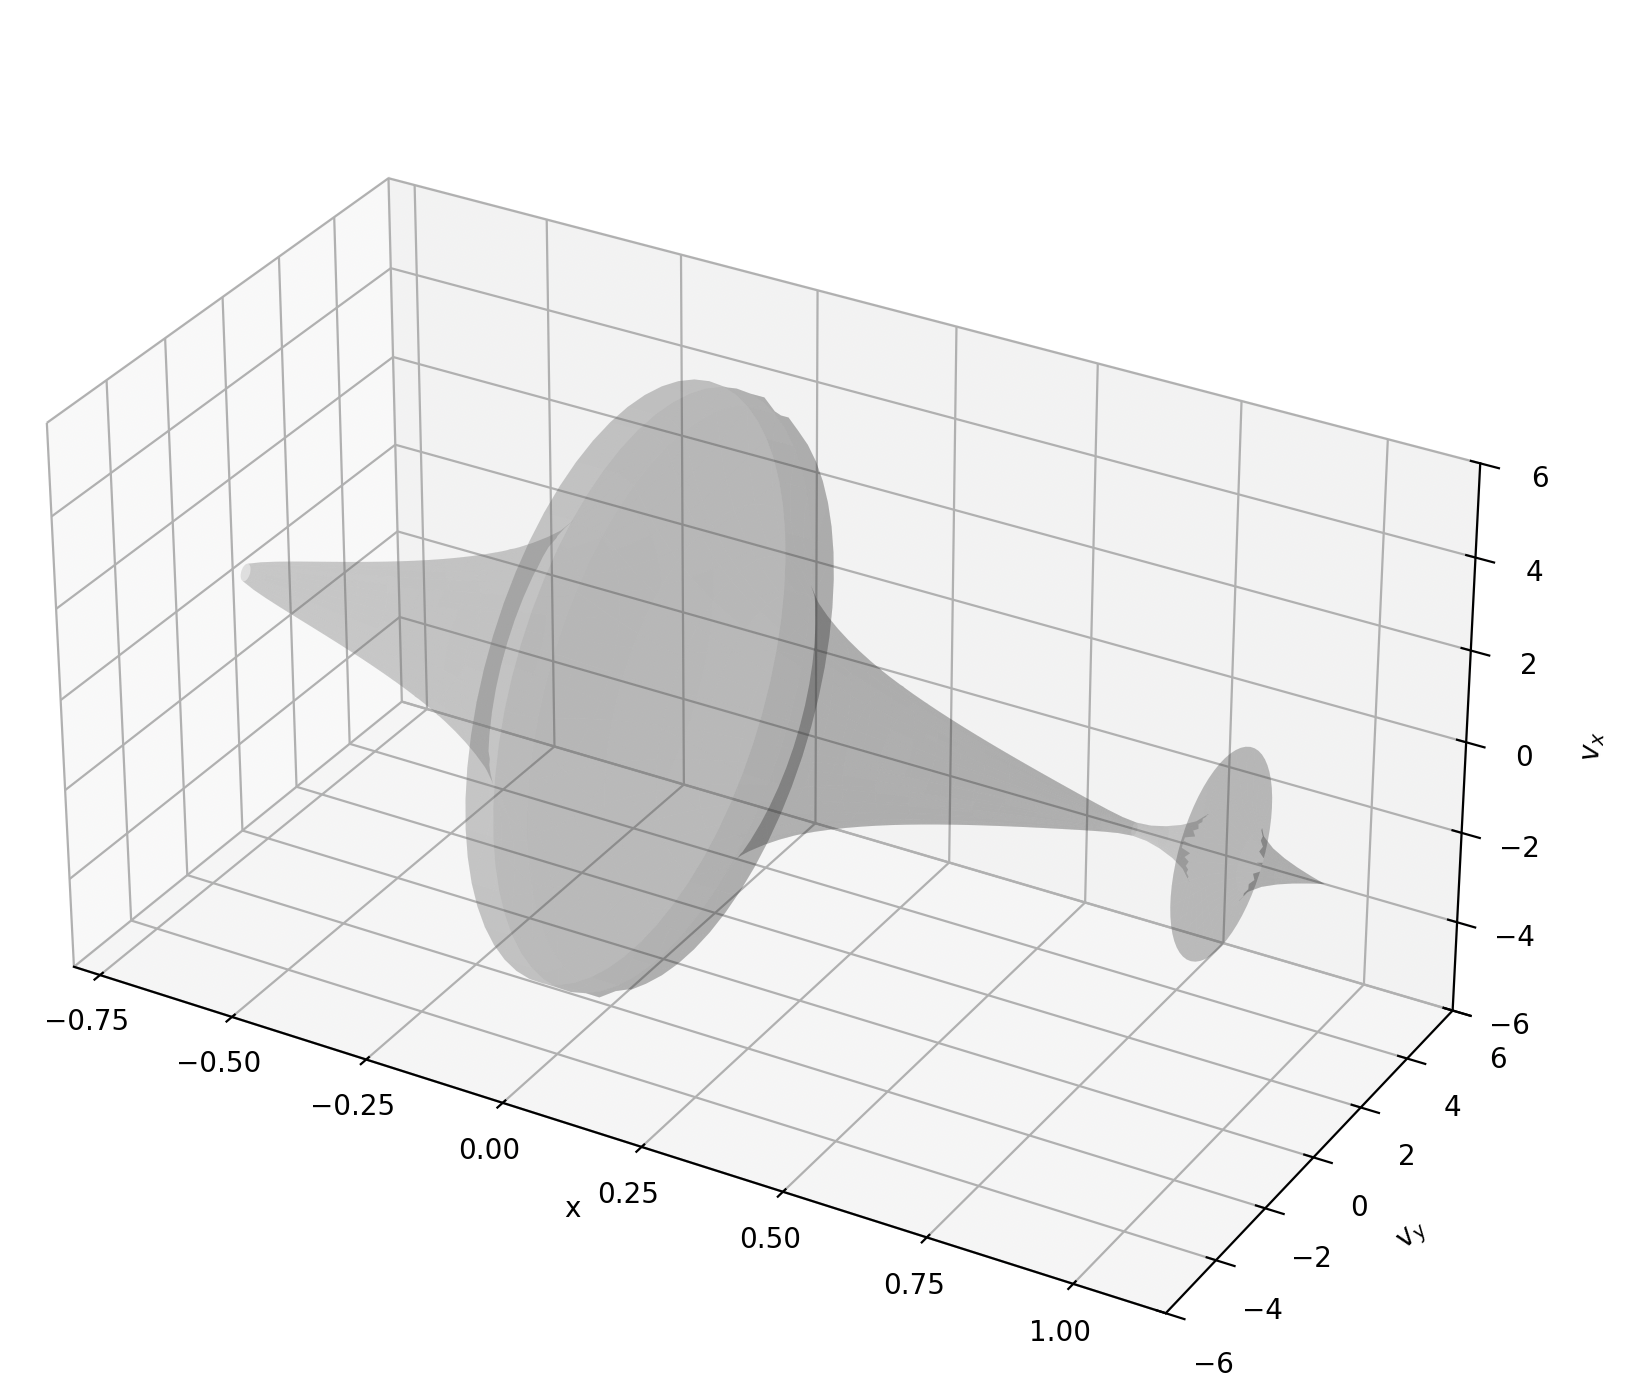
\includegraphics[width=3.1in]{images/Accessible Region 3D.png}
    %     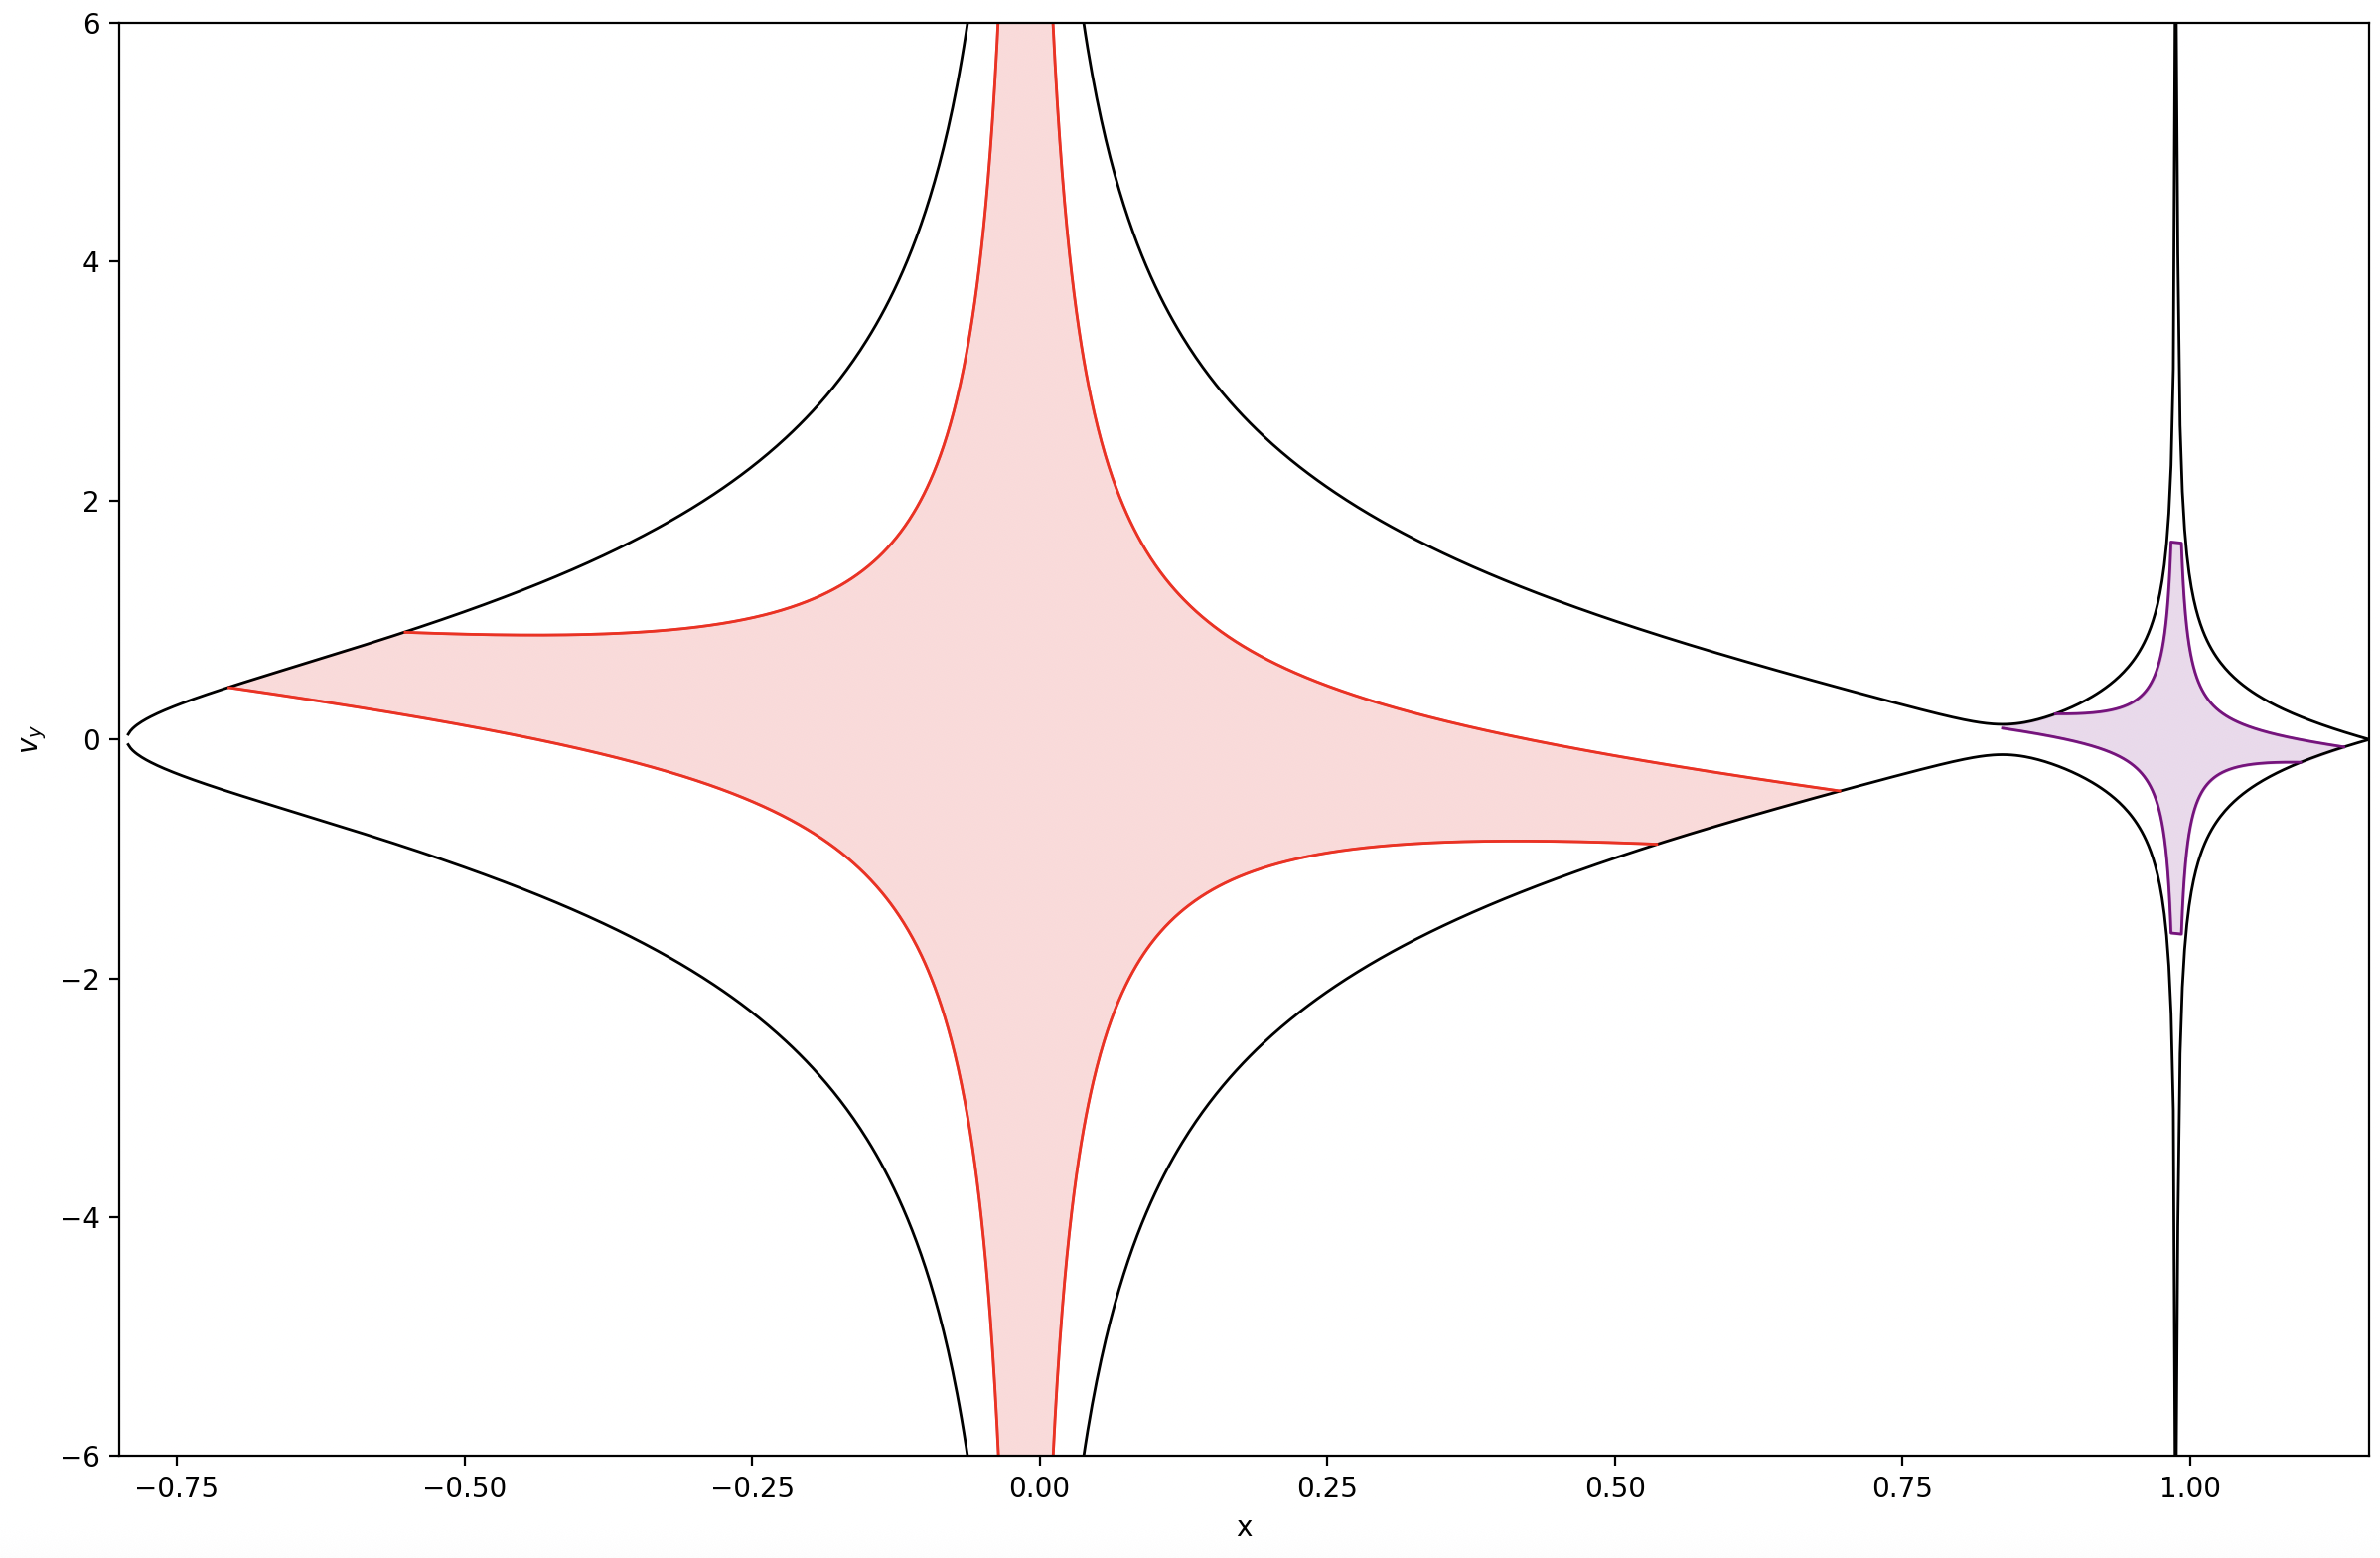
\includegraphics[width=3.2in]{images/2D accessible region with crash regions.png}
    %     \caption{Visualisations of the accessible region in three dimensions and its projection to the $(x,v_y)$ plane, displaying the Earth and Moon crash regions.}
    % \end{figure}

    
    \begin{figure}[tb]
    	\centering
        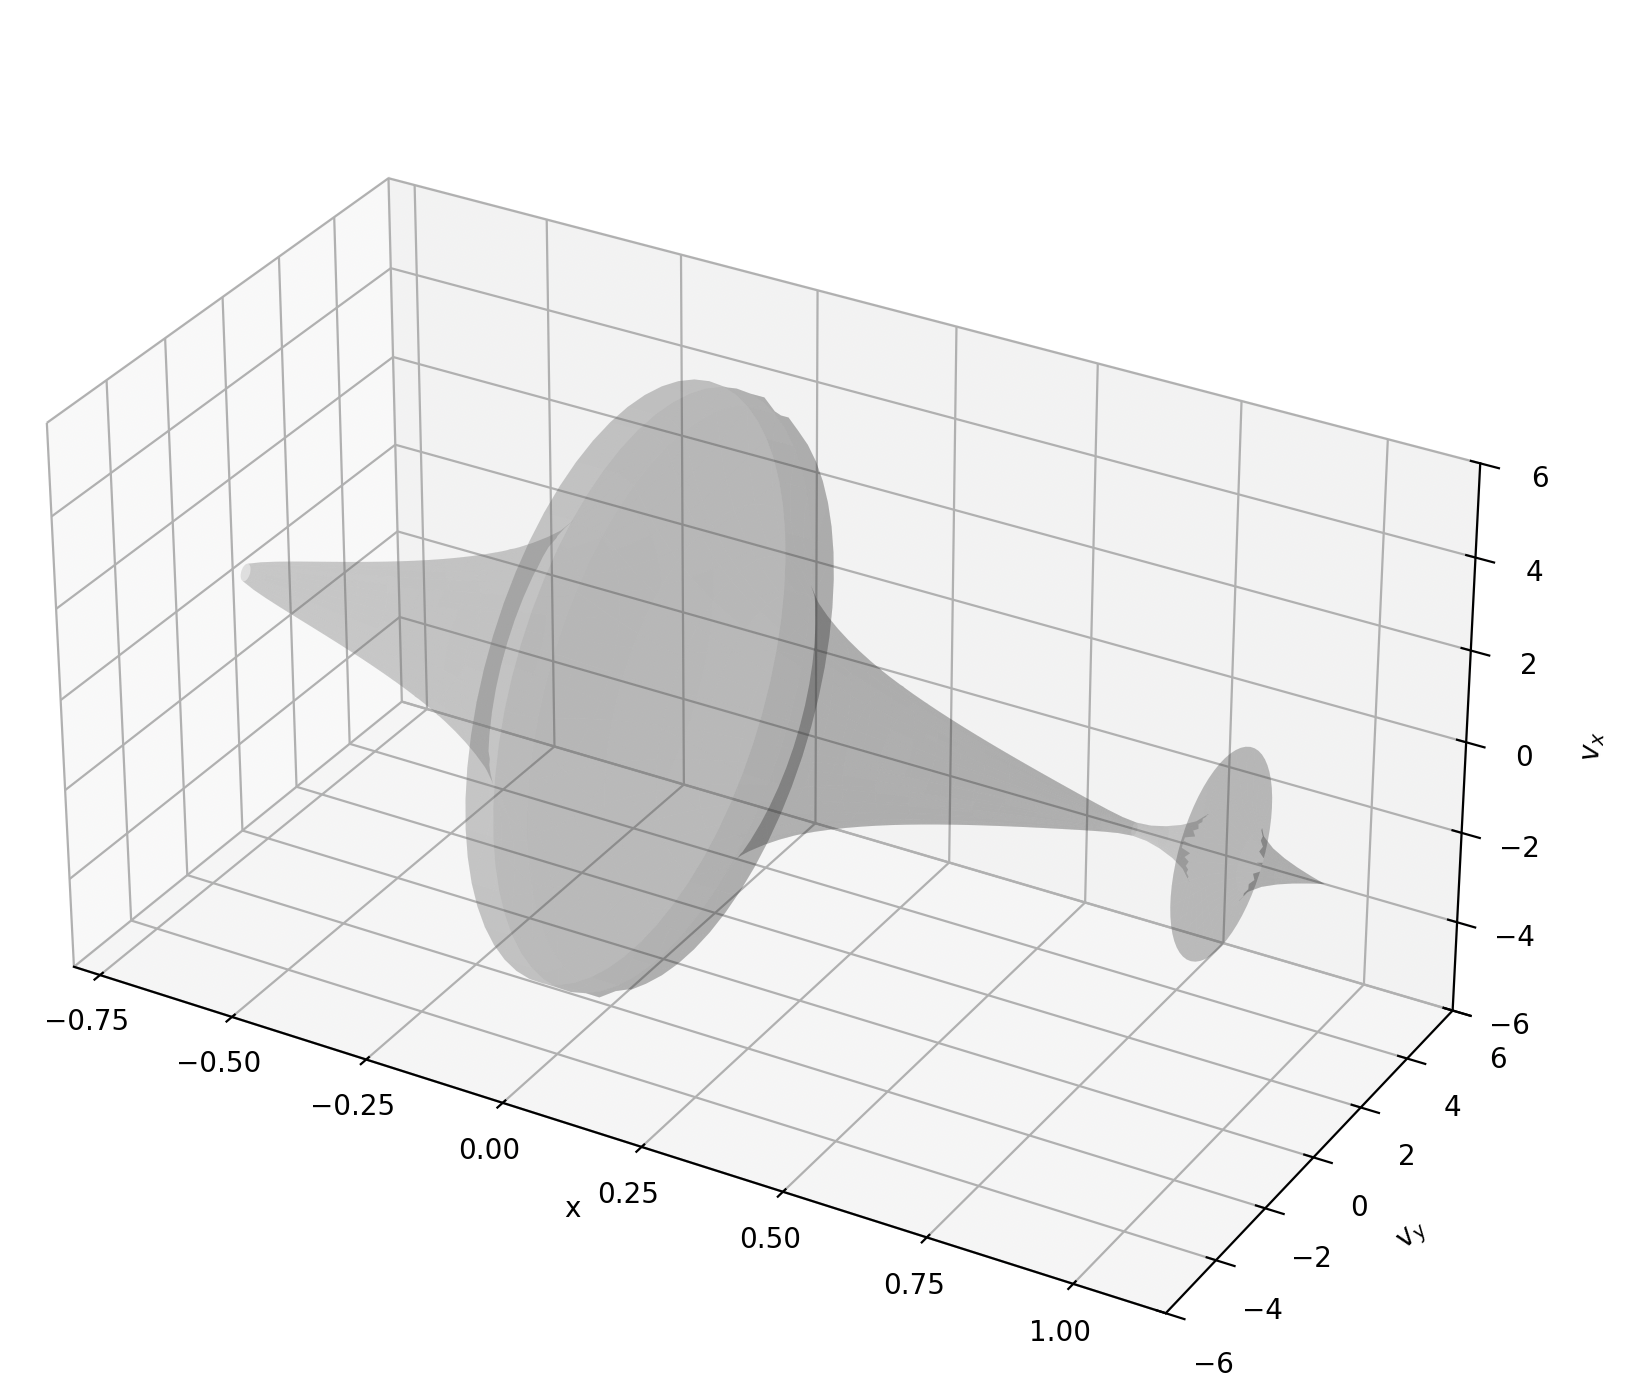
\includegraphics[width=3.1in]{images/Accessible Region 3D.png}
        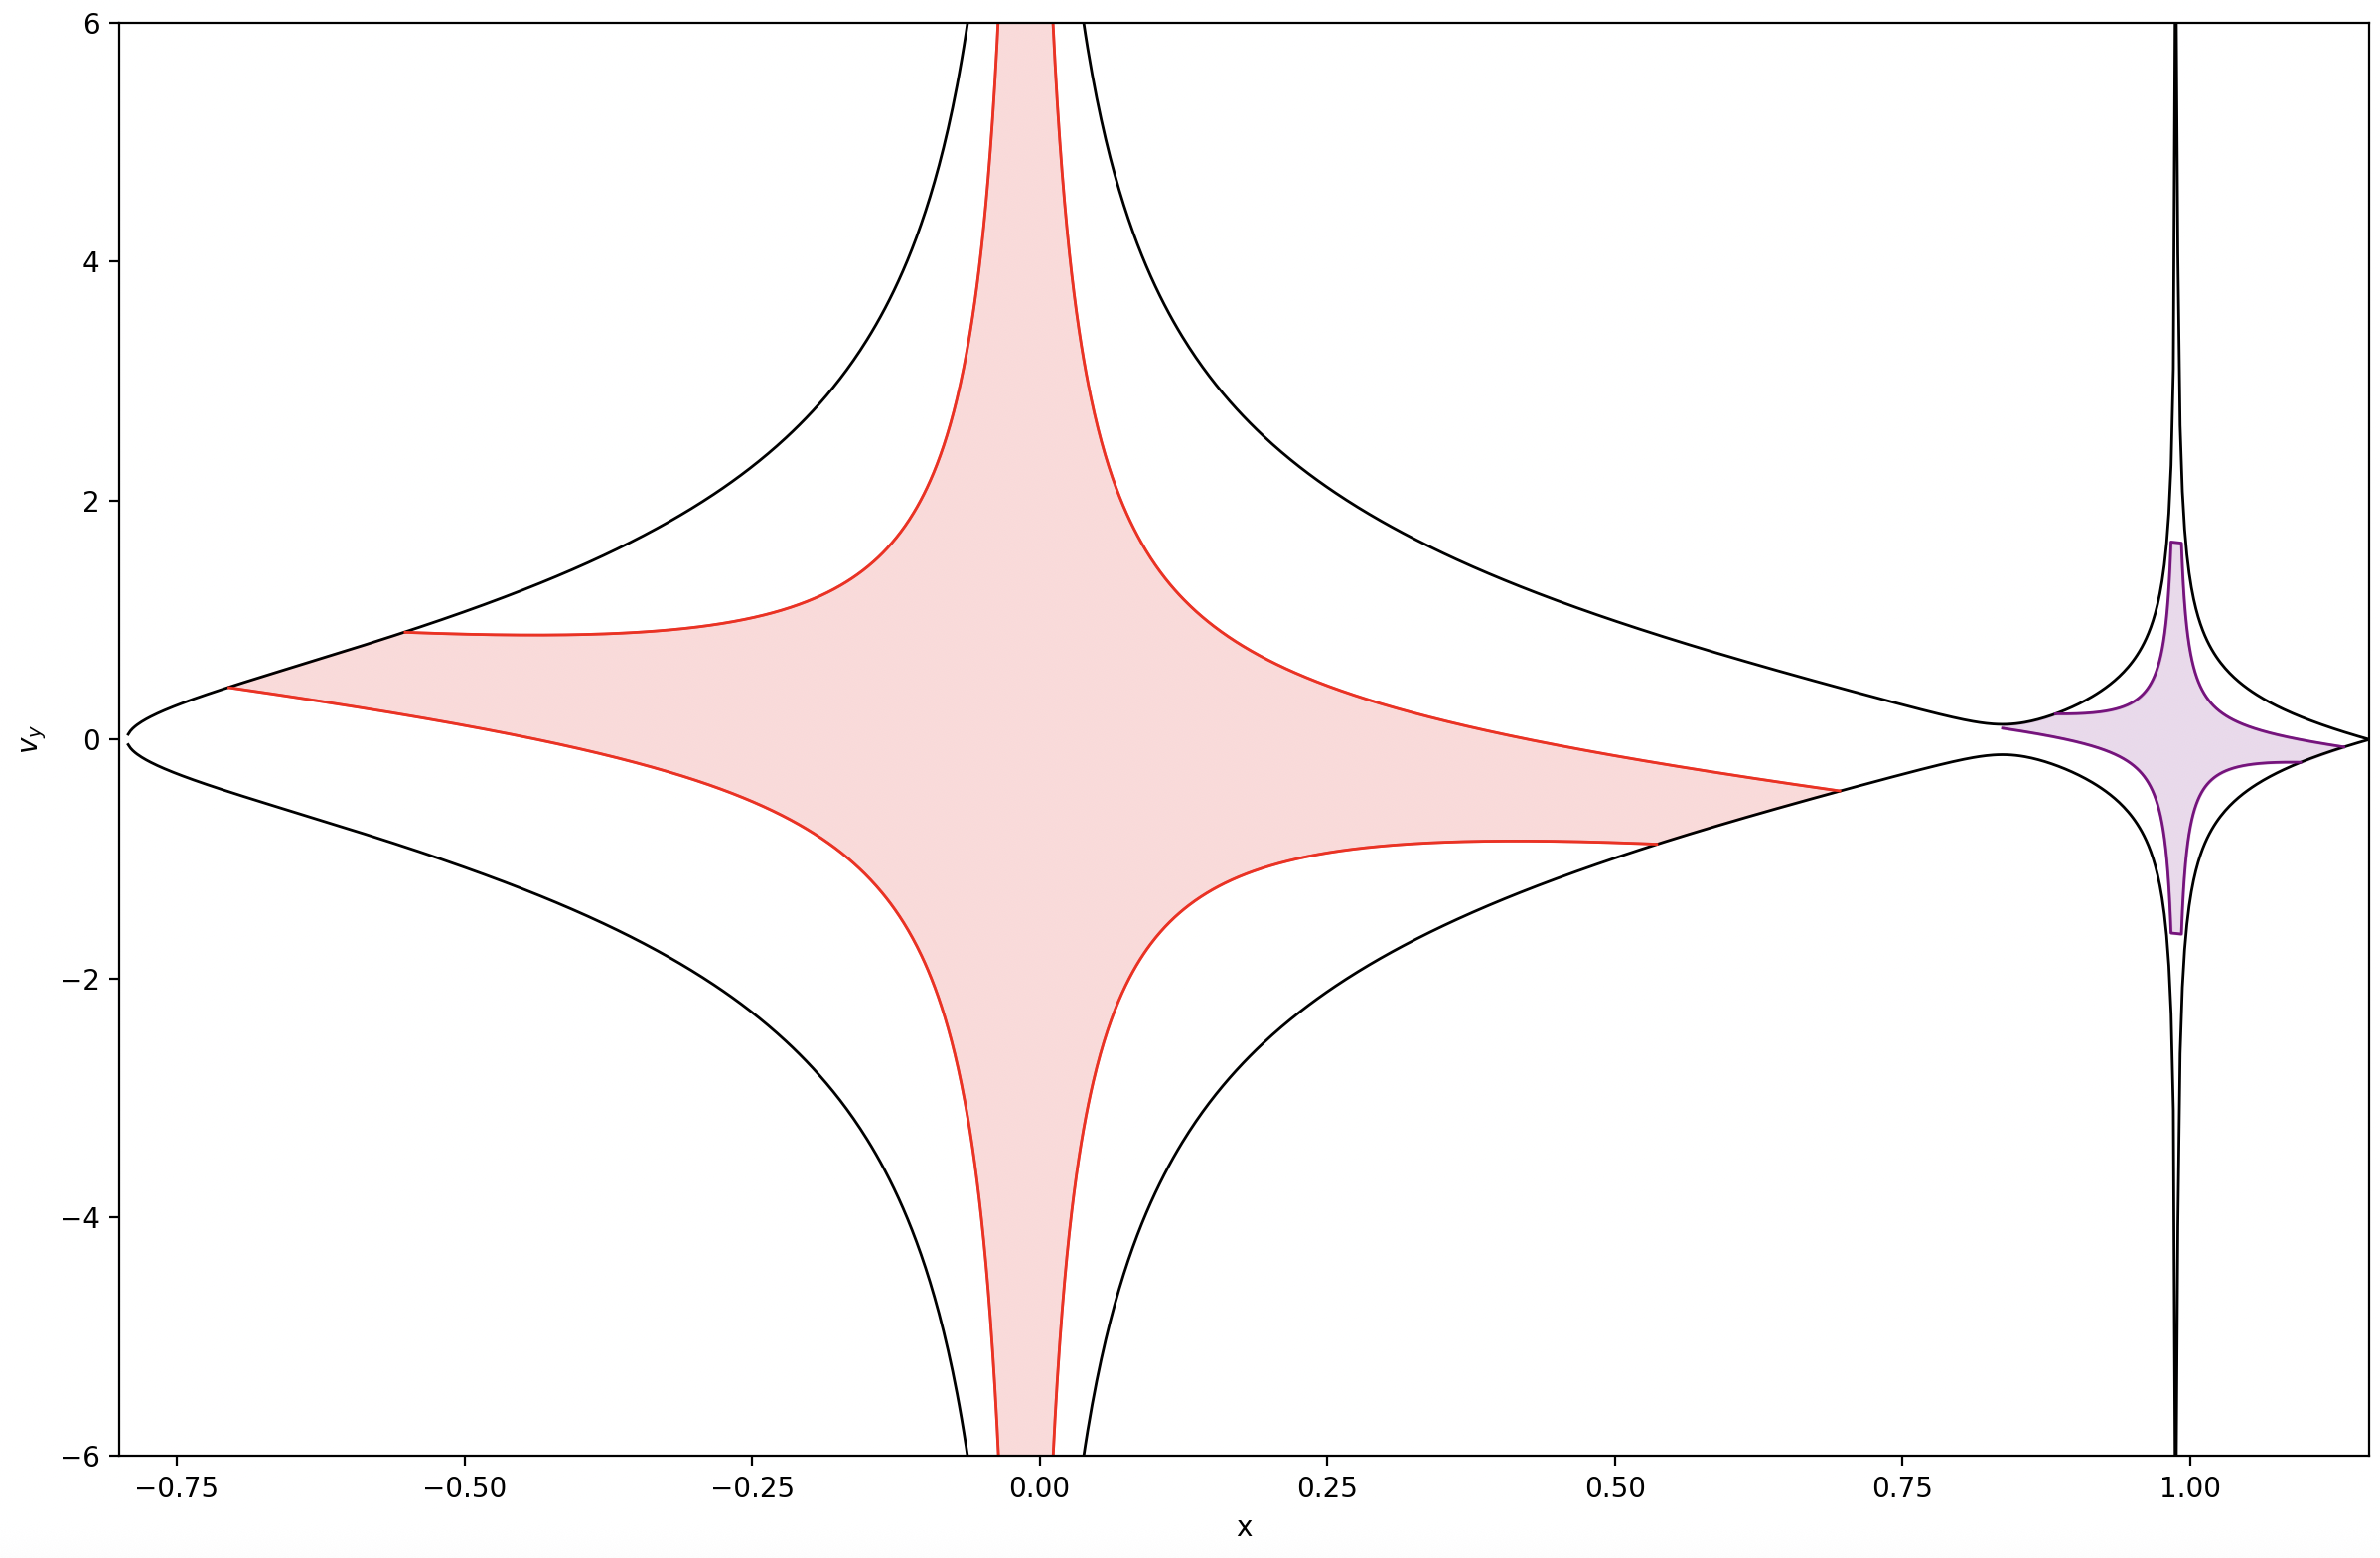
\includegraphics[width=3.2in]{images/2D accessible region with crash regions.png}
        \caption{Visualisations of the accessible region in three dimensions and its projection to the $(x,v_y)$ plane, displaying the Earth and Moon crash regions in red and purple, respectively.}
        \label{fig:accesible region 3D and 2D}
    \end{figure}








    \subsection{The crash region}



    % For certain initial conditions, an orbiting body may quickly enter Earth's atmosphere or crash into the lunar surface. From a practical perspective, points in the state space corresponding to the initial values of such orbits

    % % For certain initial conditions, an orbiting body may quickly enter Earth's atmosphere or crash into the lunar surface. From a practical perspective, points in the state space that will lead to such outcomes when taken as initial conditions are not very interesting, as our object will quickly de-orbit under them.



    For certain initial conditions, an orbiting body may quickly enter Earth's atmosphere or crash into the lunar surface. From a practical perspective, points in the state space leading to these outcomes are not very interesting (or at least, need little consideration), as an object will quickly de-orbit when placed under initial conditions corresponding to them.



    % Arbitrarily, we categorise all points leading to these results within \textit{one} orbital period 





%     We construct a set consisting of all points that will lead to such results within a single orbital period, and refer to it as the \textit{crash region}. The choice of a \textit{single} orbital period is arbitrary, but is chosen due to its convention in relevant literature.
% %
%     Indeed, in the two-dimensionally projected case, this region is analytically derived in \cite{Abraham_Marsden_1987} as the area bounded by the curve
%     \vspace{-0.4cm}
%     \begin{equation} \label{eq:crashRegion}
%     	(v_y + x)^2 =  \frac{R_i^2 v_x^2 + 2 \mu_i R_i \Bigl( 1 - \frac{R_i}{|x-x_i|}\Bigr)}{|x-x_i|^2 - R_i^2},
%     \end{equation}
%      where $\mu_1 = 1-\mu$, $\mu_2 = \mu$ are defined in terms of the normalized mass ratio, \cref{eq:mass ratio}, of the Earth and Moon, $R_1 \approx 7000$, $R_2 = 1738.1$ are the radii of the Earth (including significant portions of the atmosphere) and Moon in kilometres, and $x_1, x_2$ are the distances of the Earth/Moon from the system barycentre, respectively. The Earth and Moon crash regions can both be seen in \cref{fig:accesible region 3D and 2D}.
    



    % We construct a set consisting of all points that will lead to such results within a single orbital period, and refer to it as the \textit{crash region}. The choice of a \textit{single} orbital period is arbitrary, but is chosen due to its convention in relevant literature.
    We construct a set consisting of all points that will lead to such results, and refer to it as the \textit{crash region}.
%
    Indeed, in the two-dimensionally projected case, this region is analytically derived in \cite{Graebner2025}, using techniques from \cite{Abraham_Marsden_1987}, as the area bounded by the curve
    \vspace{-0cm}
    \begin{equation} \label{eq:crashRegion}
    	(v_y + x)^2 =  \frac{R_i^2 v_x^2 + 2 \mu_i R_i \Bigl( 1 - \frac{R_i}{|x-x_i|}\Bigr)}{|x-x_i|^2 - R_i^2},
    \end{equation}
     where $\mu_1 = 1-\mu$, $\mu_2 = \mu$ are defined in terms of the normalized mass ratio, \cref{eq:mass ratio}, of the Earth and Moon, $R_1 \approx 7000$, $R_2 = 1738.1$ are the radii of the Earth (including significant portions of the atmosphere) and Moon in kilometres, and $x_1, x_2$ are the distances of the Earth/Moon from the system barycentre, respectively. The Earth and Moon crash regions can both be seen in \cref{fig:accesible region 3D and 2D}. Previous work in \cite{Graebner2025} has numerically verified the validity of this analytically-derived region.
    













    % Following the process laid out in \cref{subsec: computationOfPlanarResonantOrbits} to compute the crossings of planar resonant orbits, code employing the use of pydylan (a Python interface to the Dynamically Leveraged Automated (N) Multibody Trajectory Optimization software \cite{beeson2022dynamically}) was written to plot these crossings within the accessible region for several different orbital families.

    % % \begin{figure}[htb]
    % % 	\centering
    % %     % 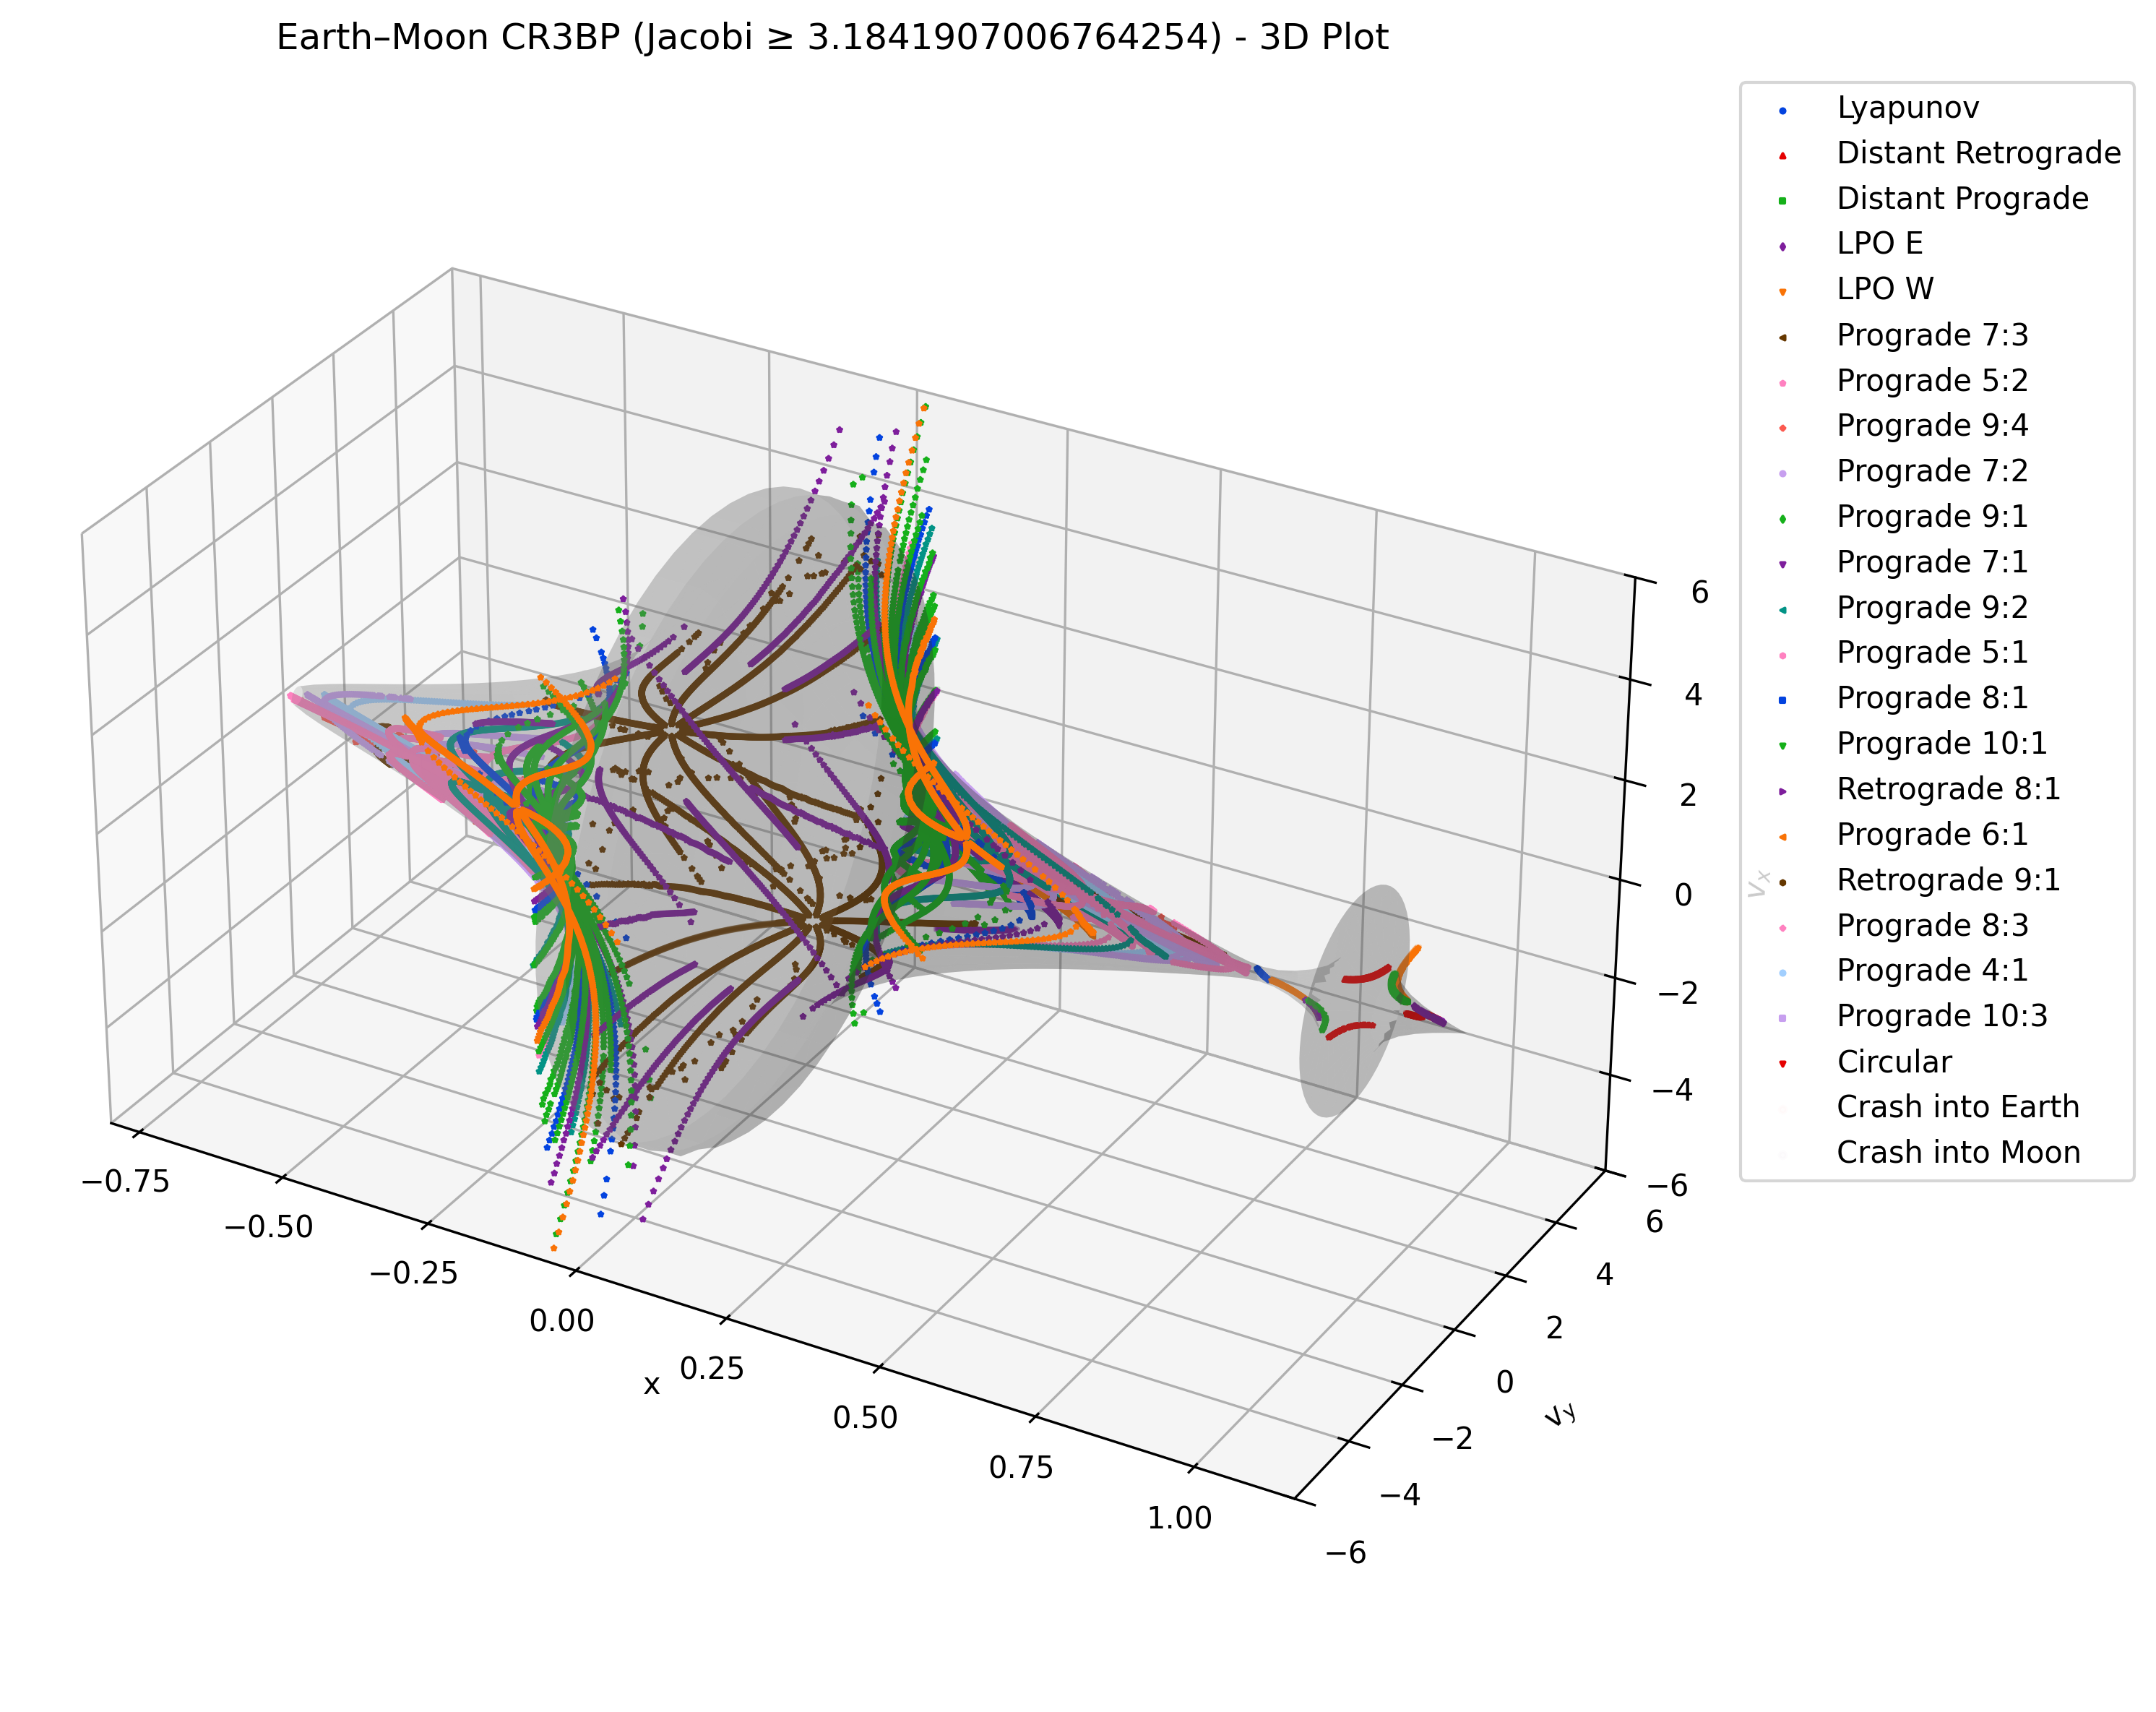
\includegraphics[width=2.9in]{images/3D crossings all orbits.png}
    % %     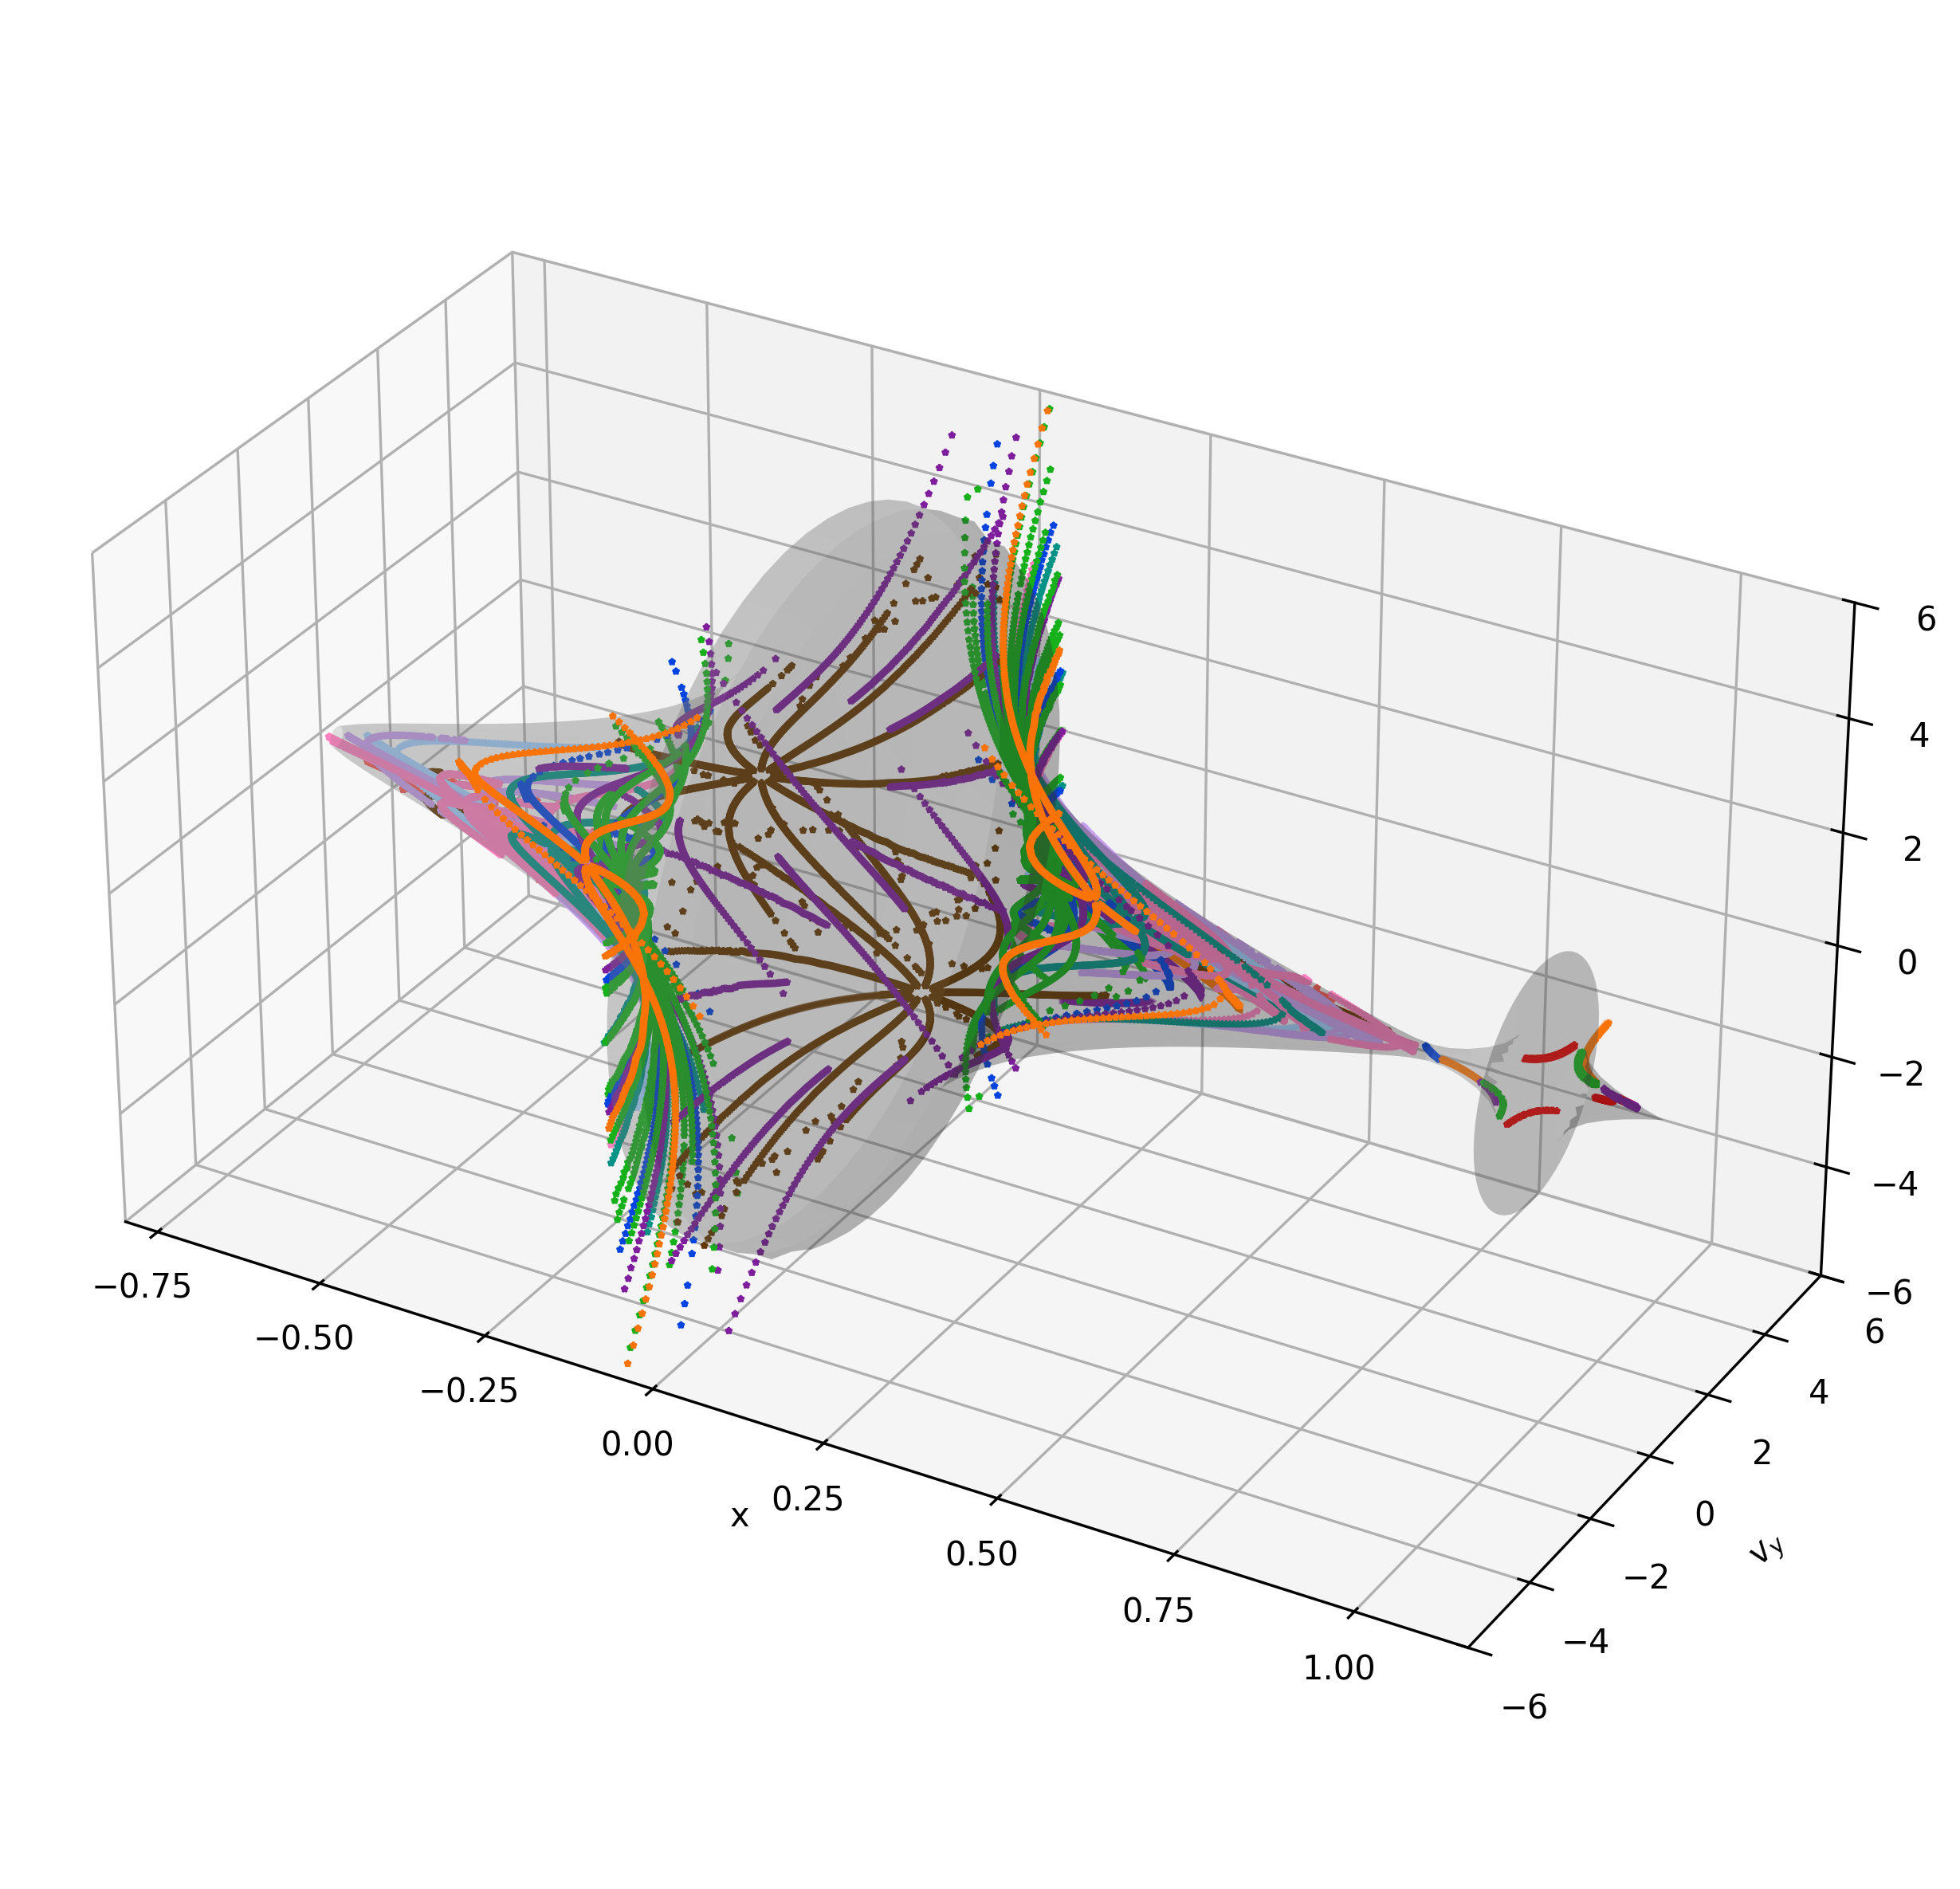
\includegraphics[width=2.9in]{images/3D crossings all orbits (without title and legend).png}
    % %     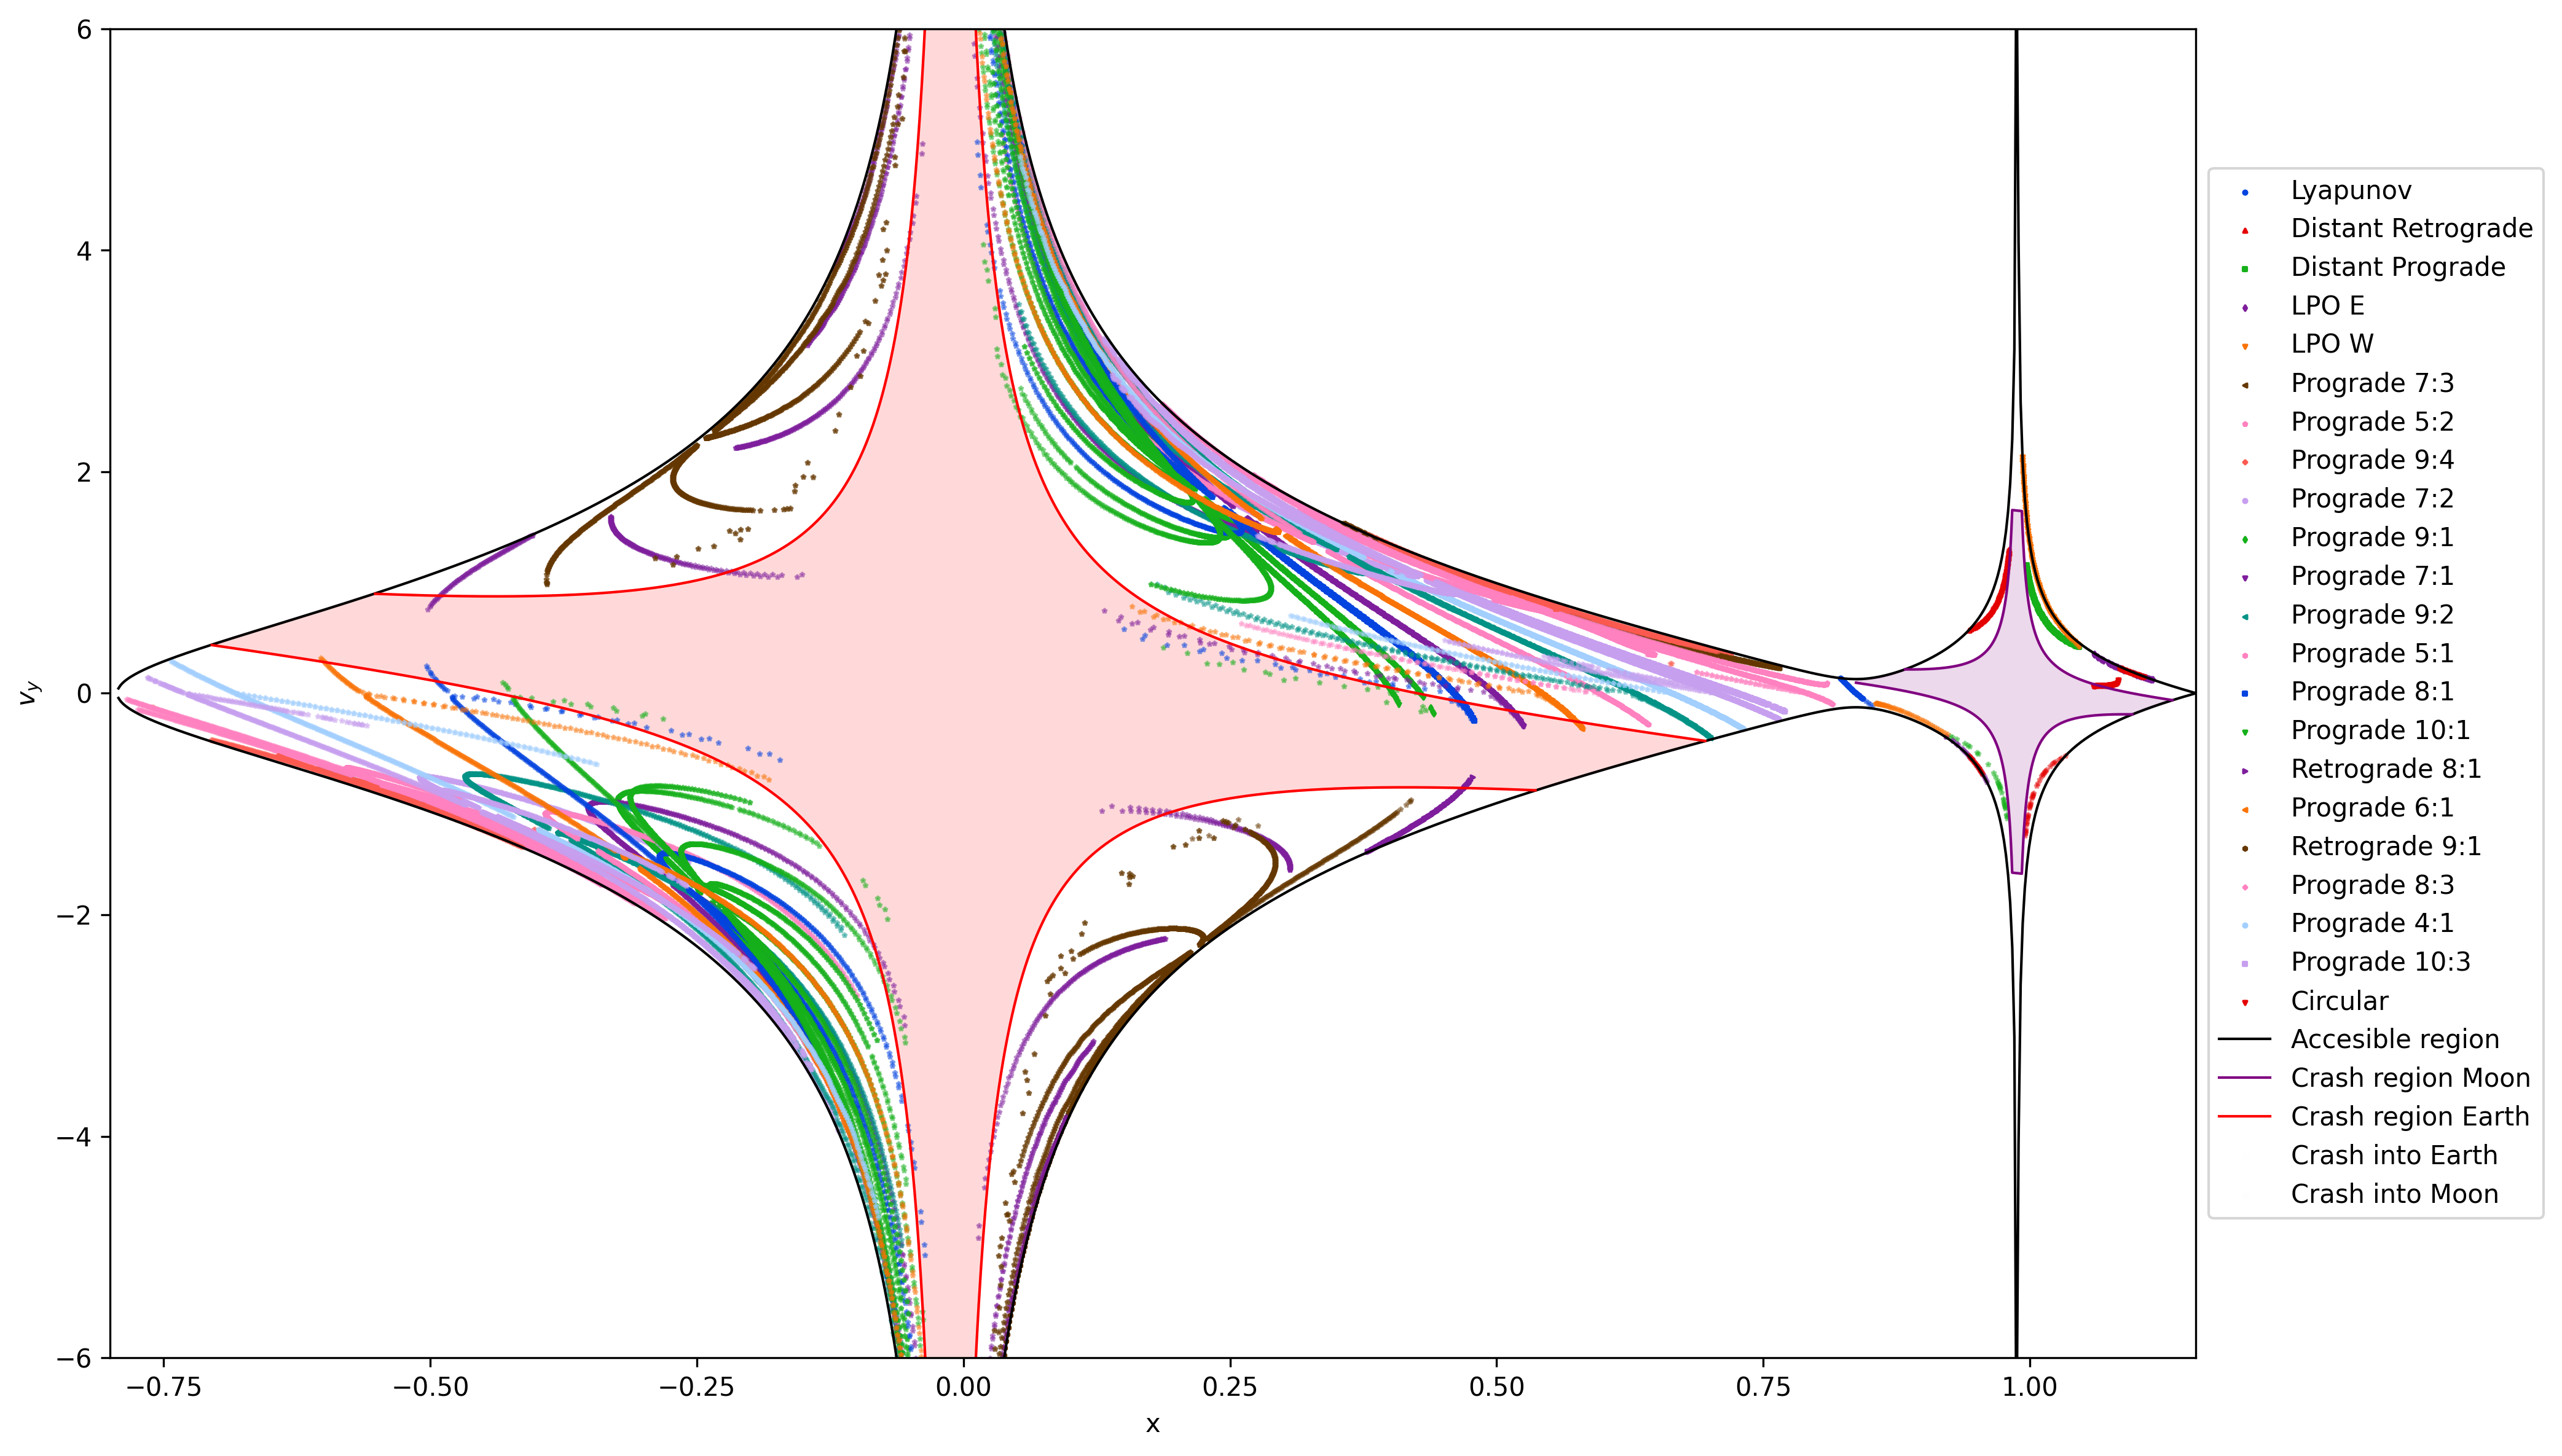
\includegraphics[width=in]{images/2D crossings all orbits.png}
    % %     \caption{Visualisations of the accessible region in three dimensions and its projection to the $(x,v_y)$ plane, displaying the Earth and Moon crash regions.}
    % % 	\label{fig:accesible region 3D and 2D}
    % % \end{figure}

    
    % \begin{figure}[htb] \label{fig:orbital crossings plotted}
    % 	\centering
    %     % 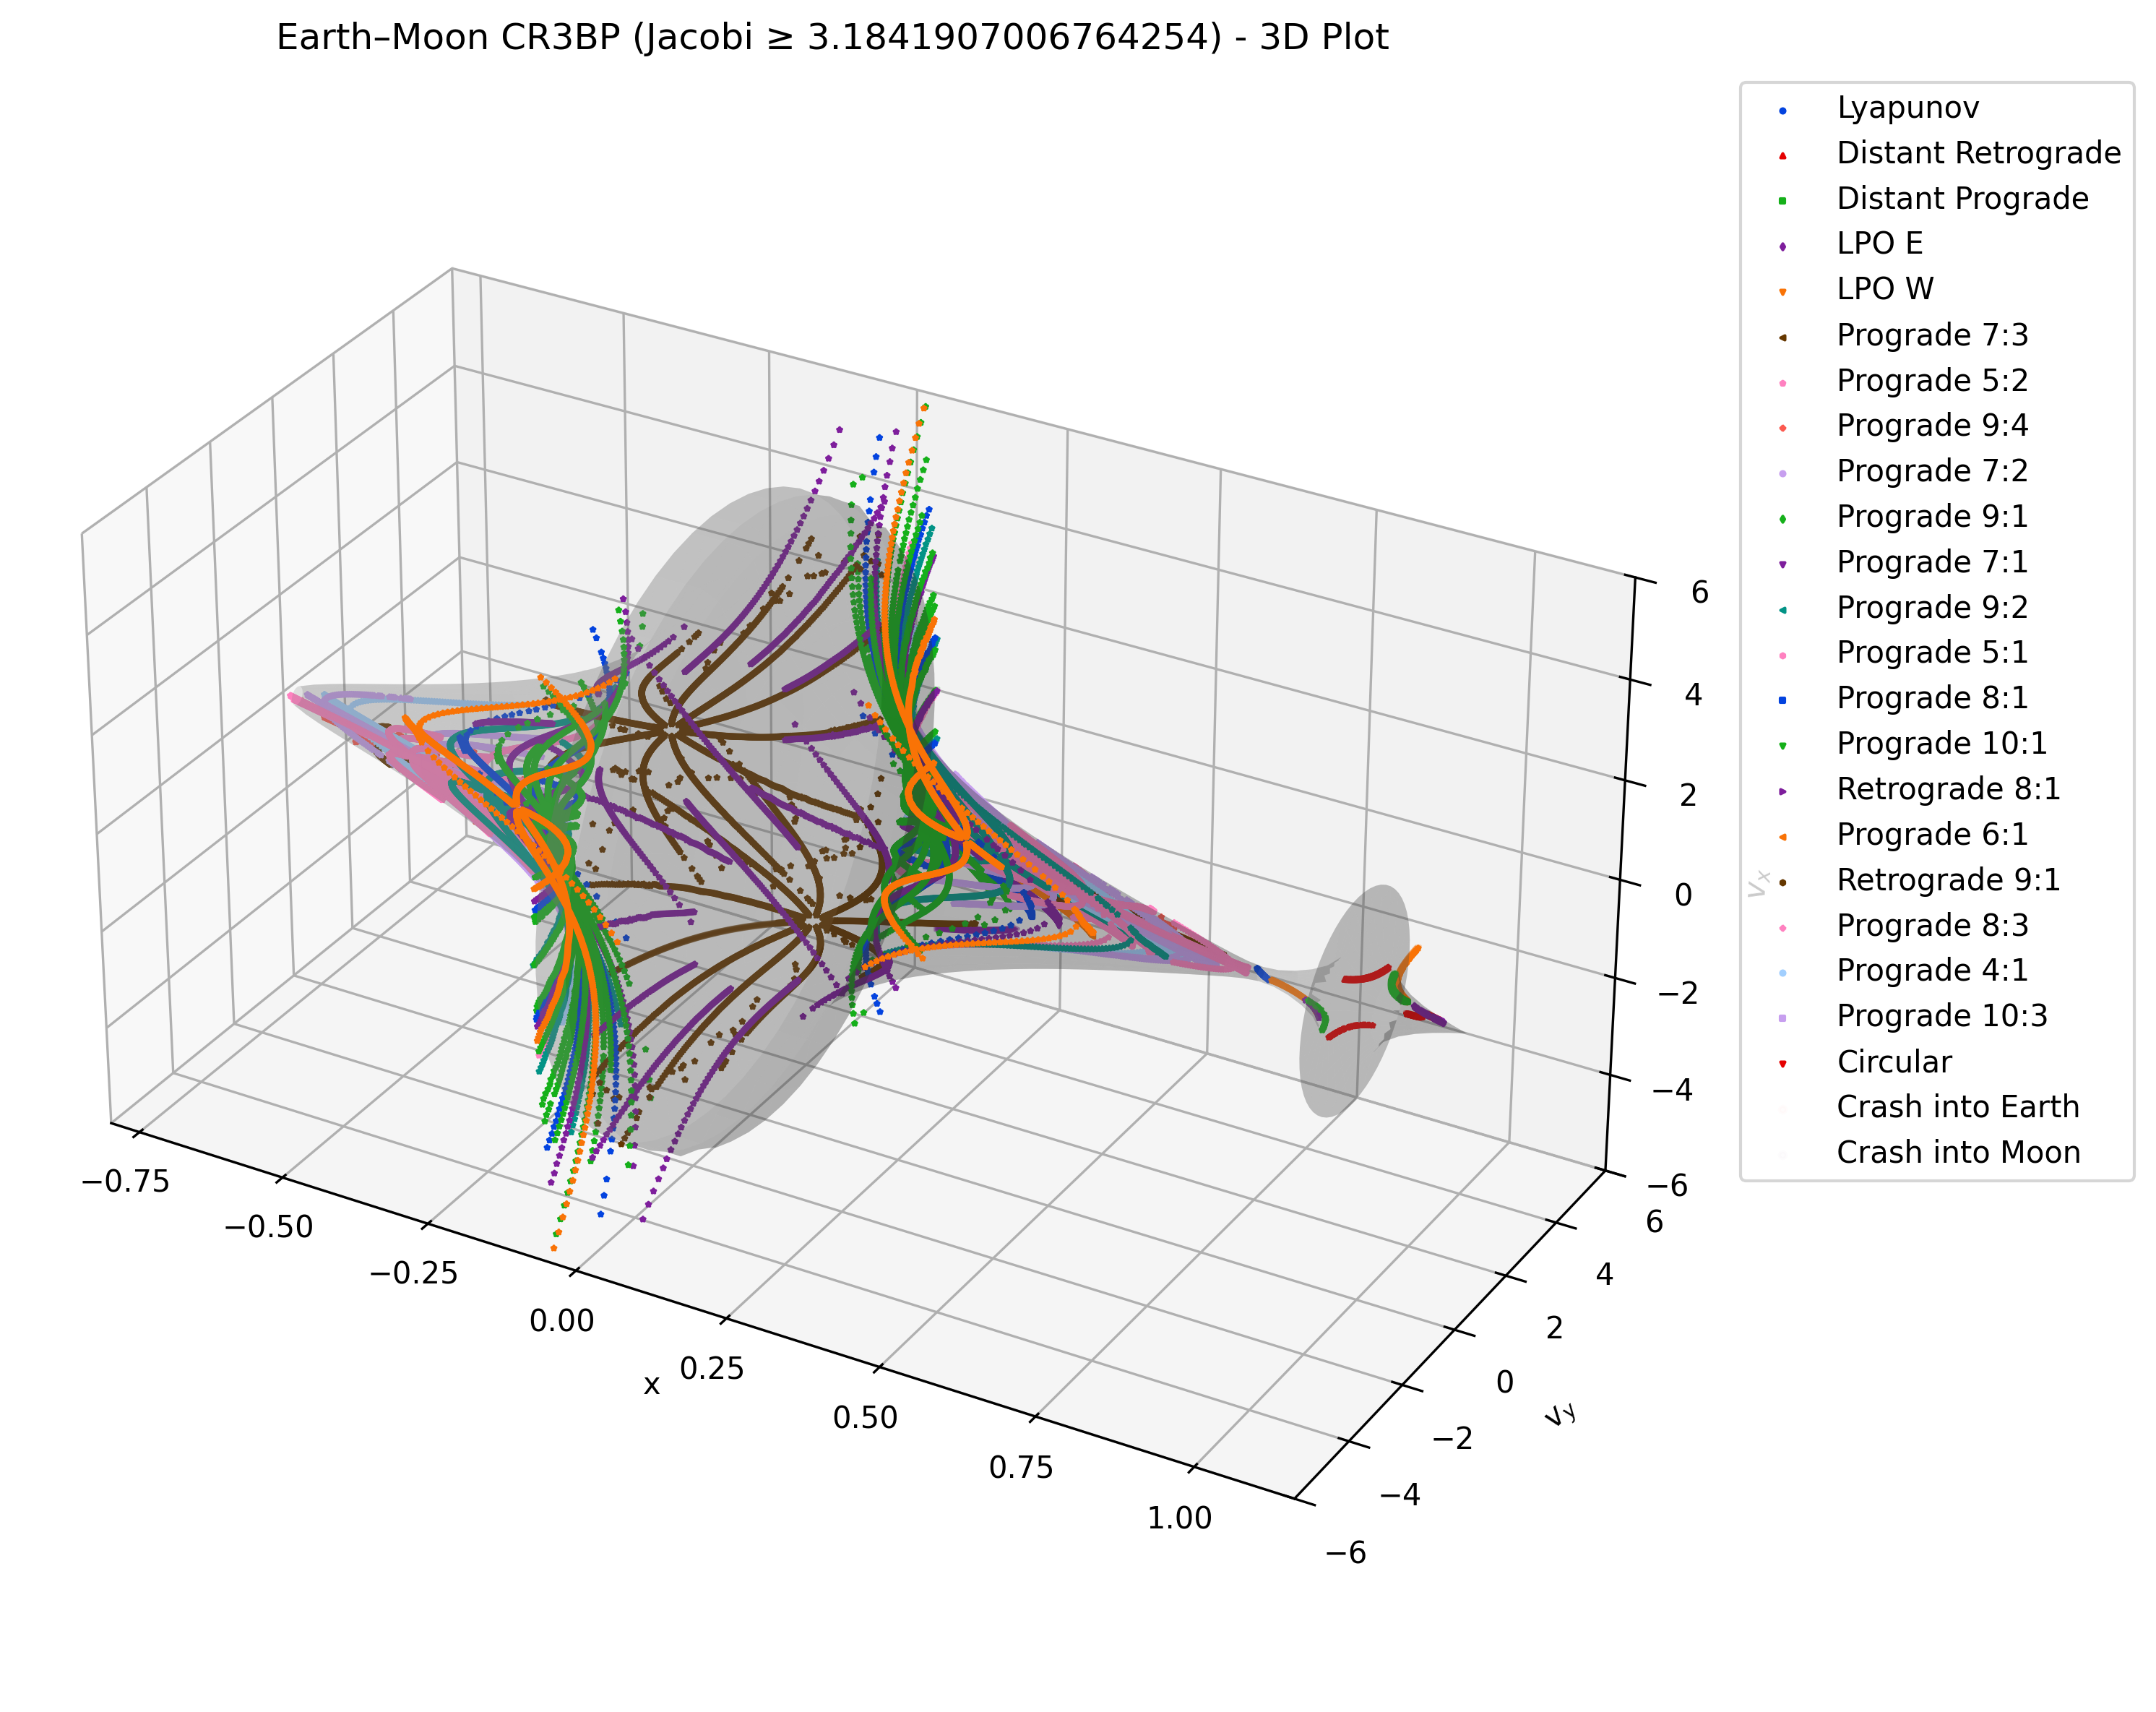
\includegraphics[width=2.9in]{images/3D crossings all orbits.png}
    %     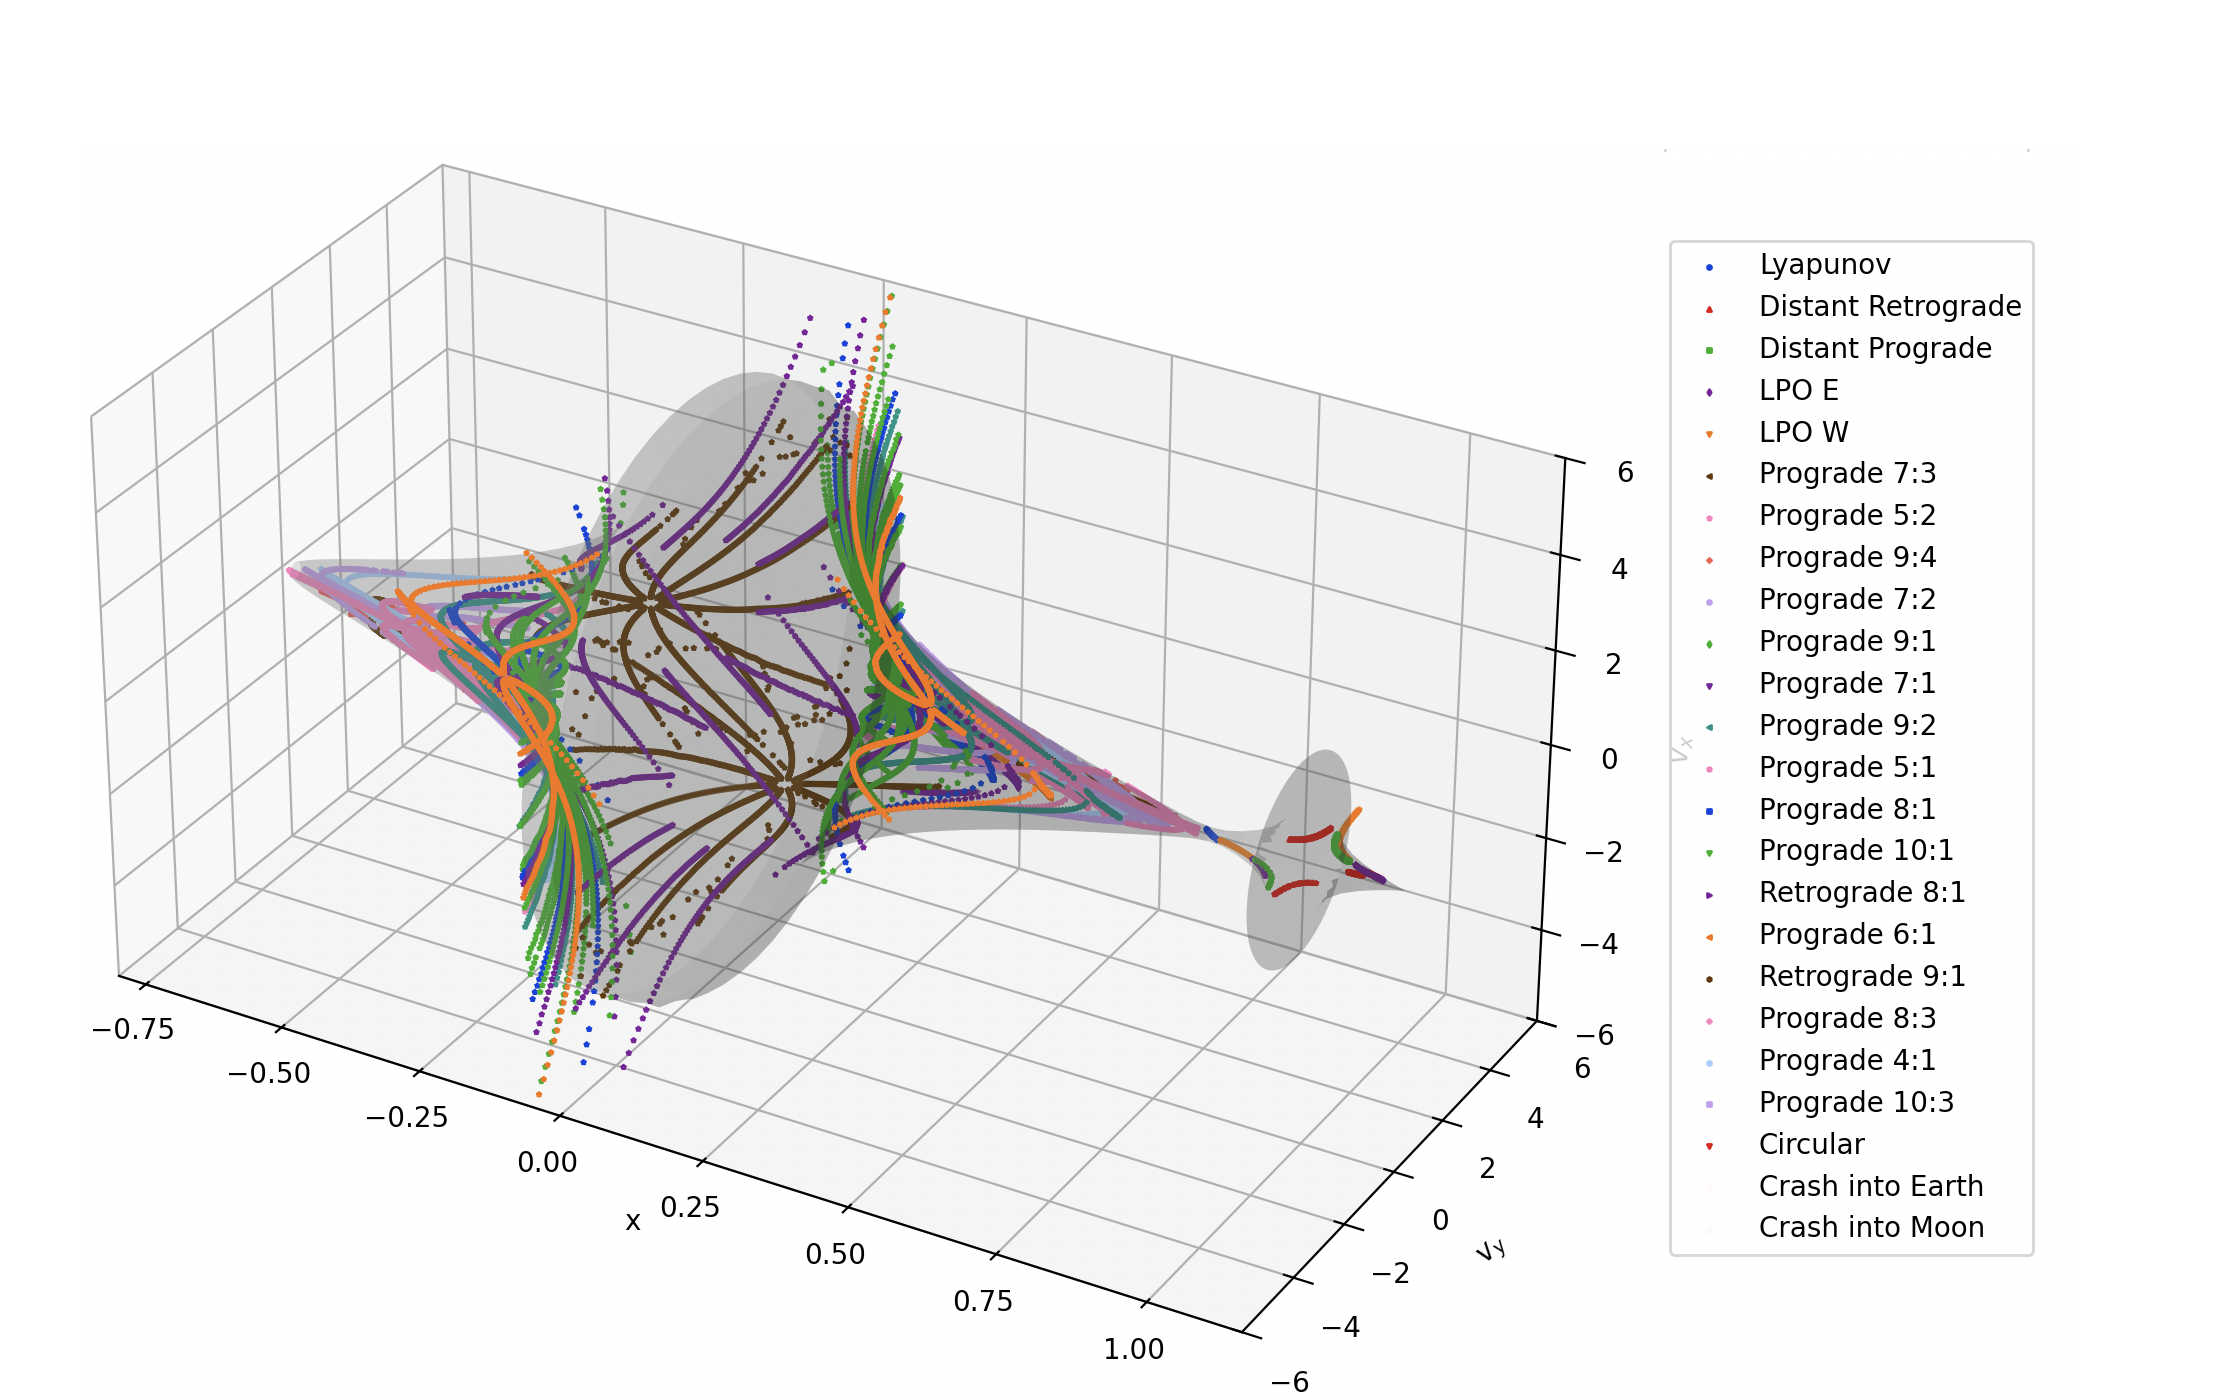
\includegraphics[width=0.85\linewidth]{images/manually made 3d.png}
    %     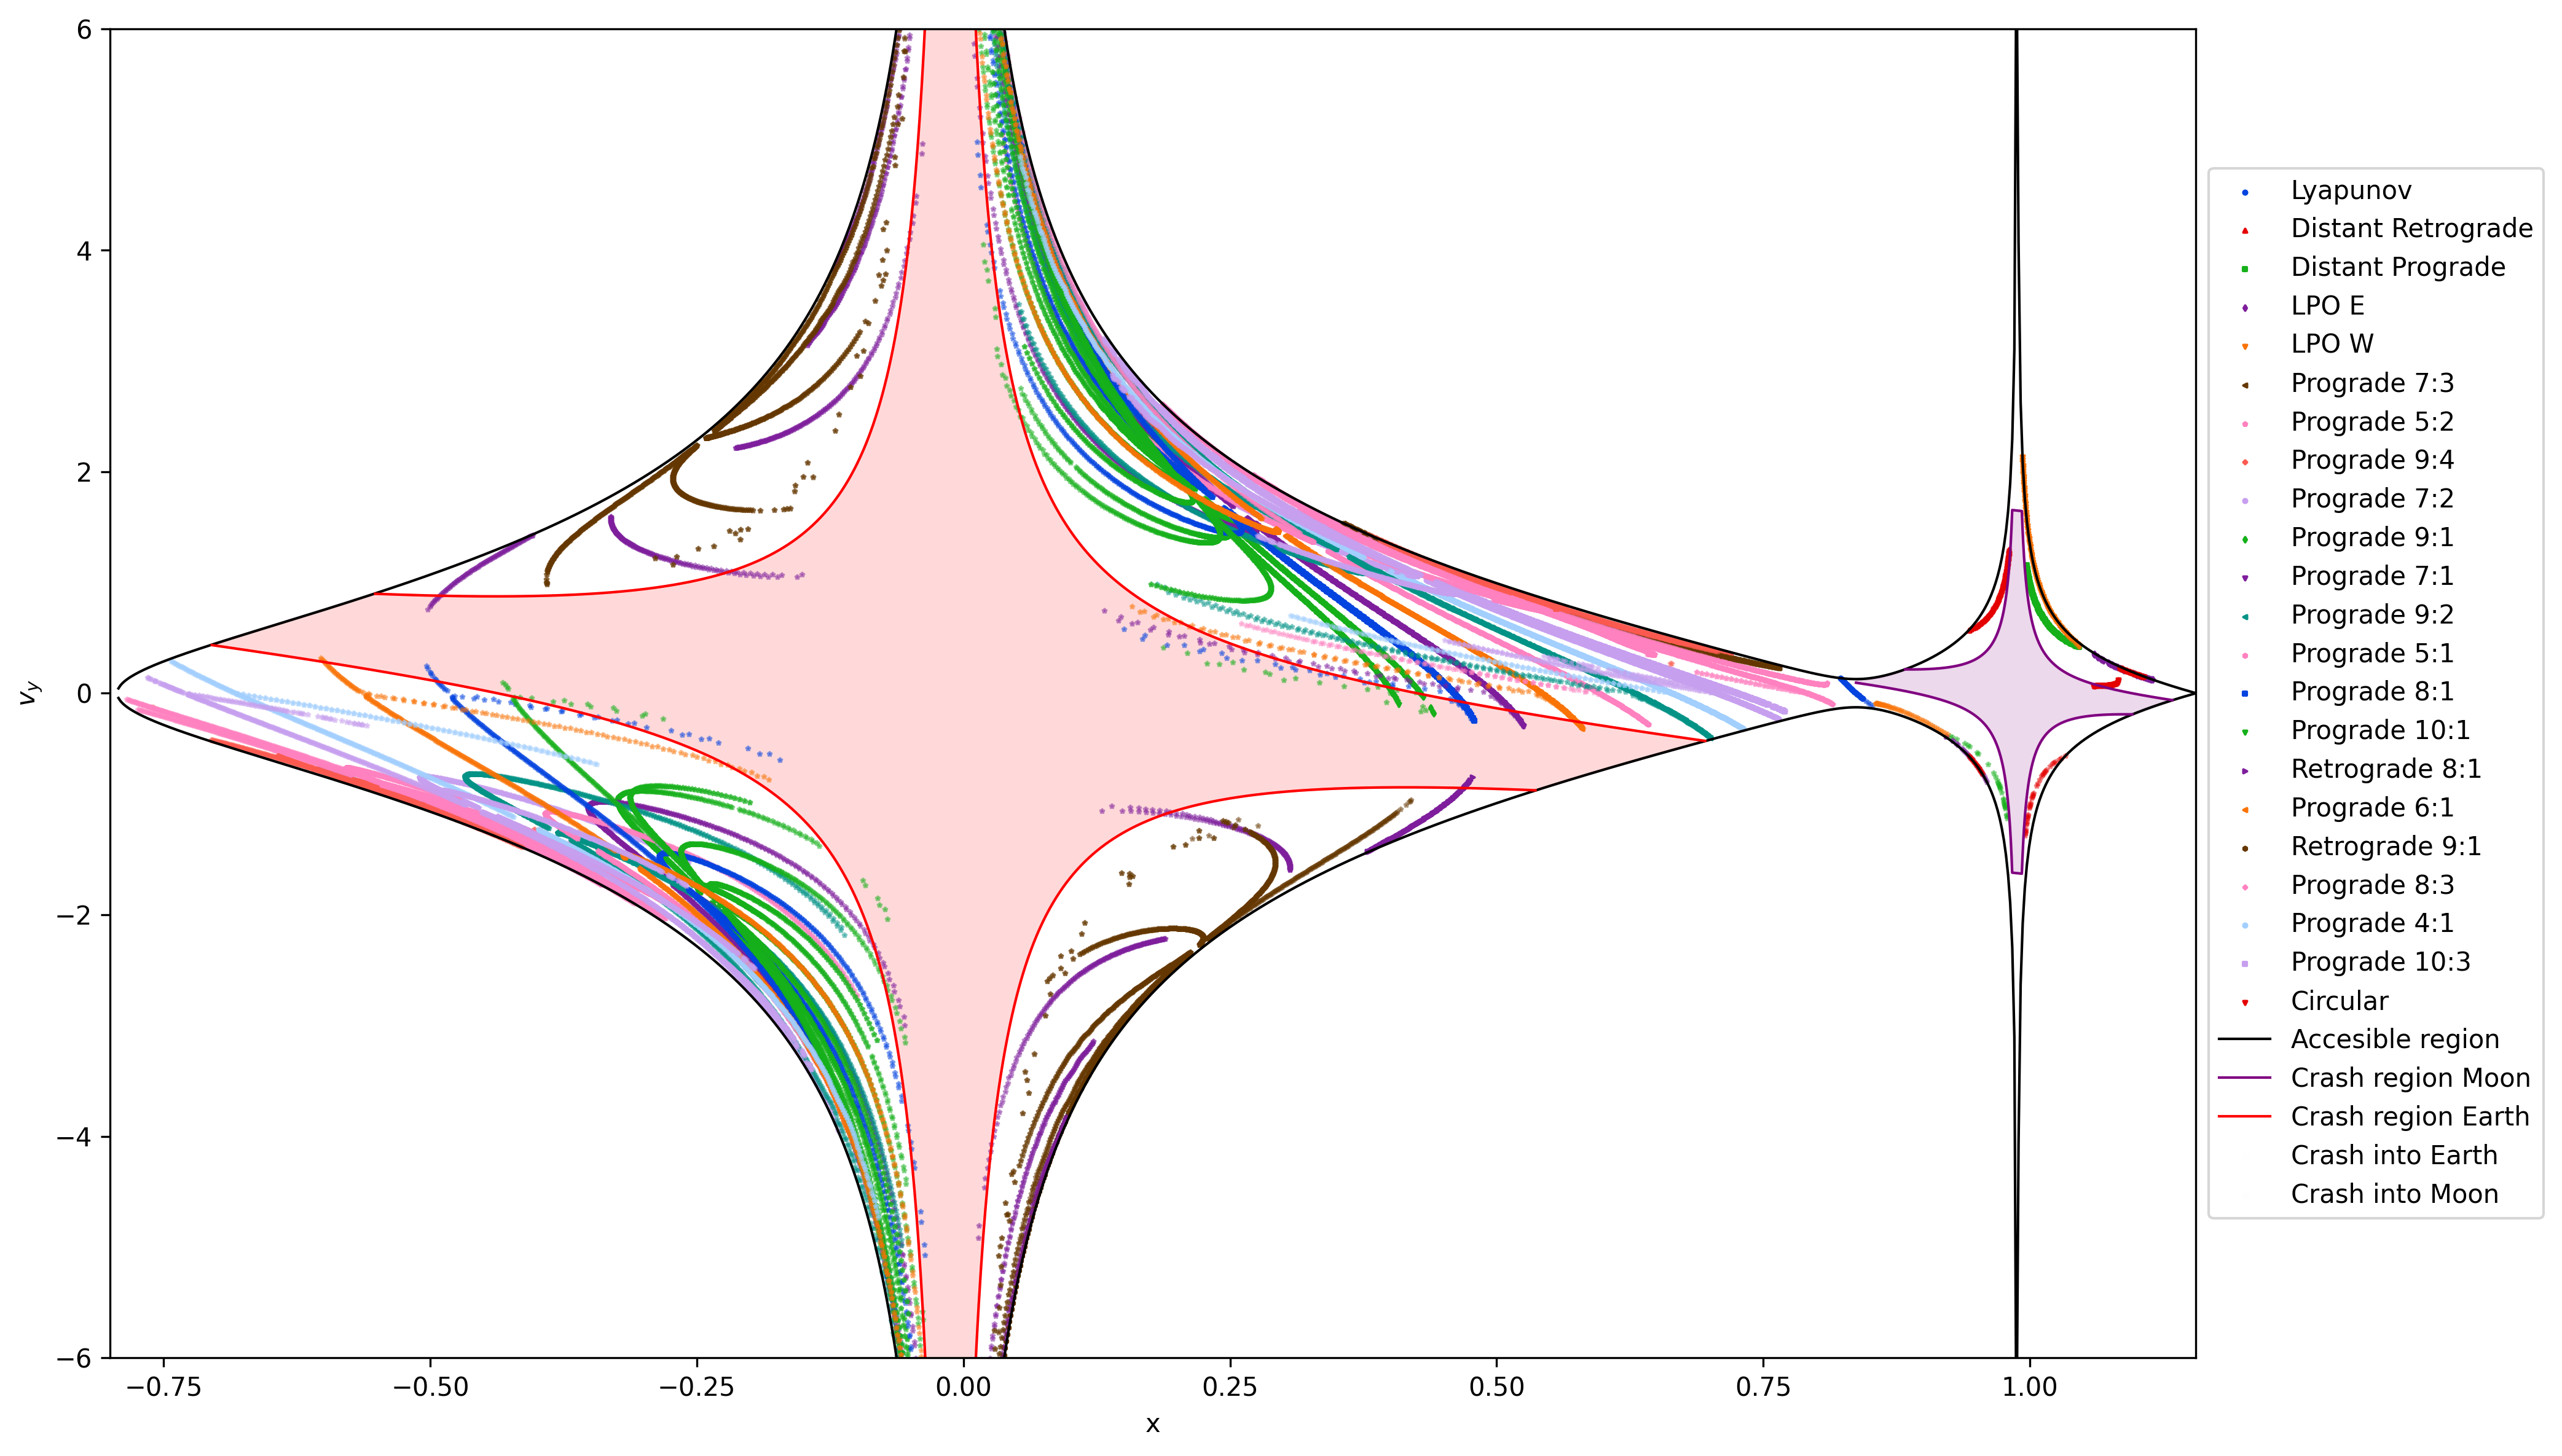
\includegraphics[width=0.75\linewidth]{images/2D crossings all orbits.png}
    %     \caption{Visualisations of the accessible region in three dimensions and its projection to the $(x,v_y)$ plane, displaying the Earth and Moon crash regions. The larger `pseudosphere'-esque region corresponds to the region around Earth, and the smaller: that of the Moon.}
    % \end{figure}



    % % \begin{figure}[htb]
    % %     \centering
    % %     \parbox[c]{2.9in}{%
    % %         % \centering
    % %         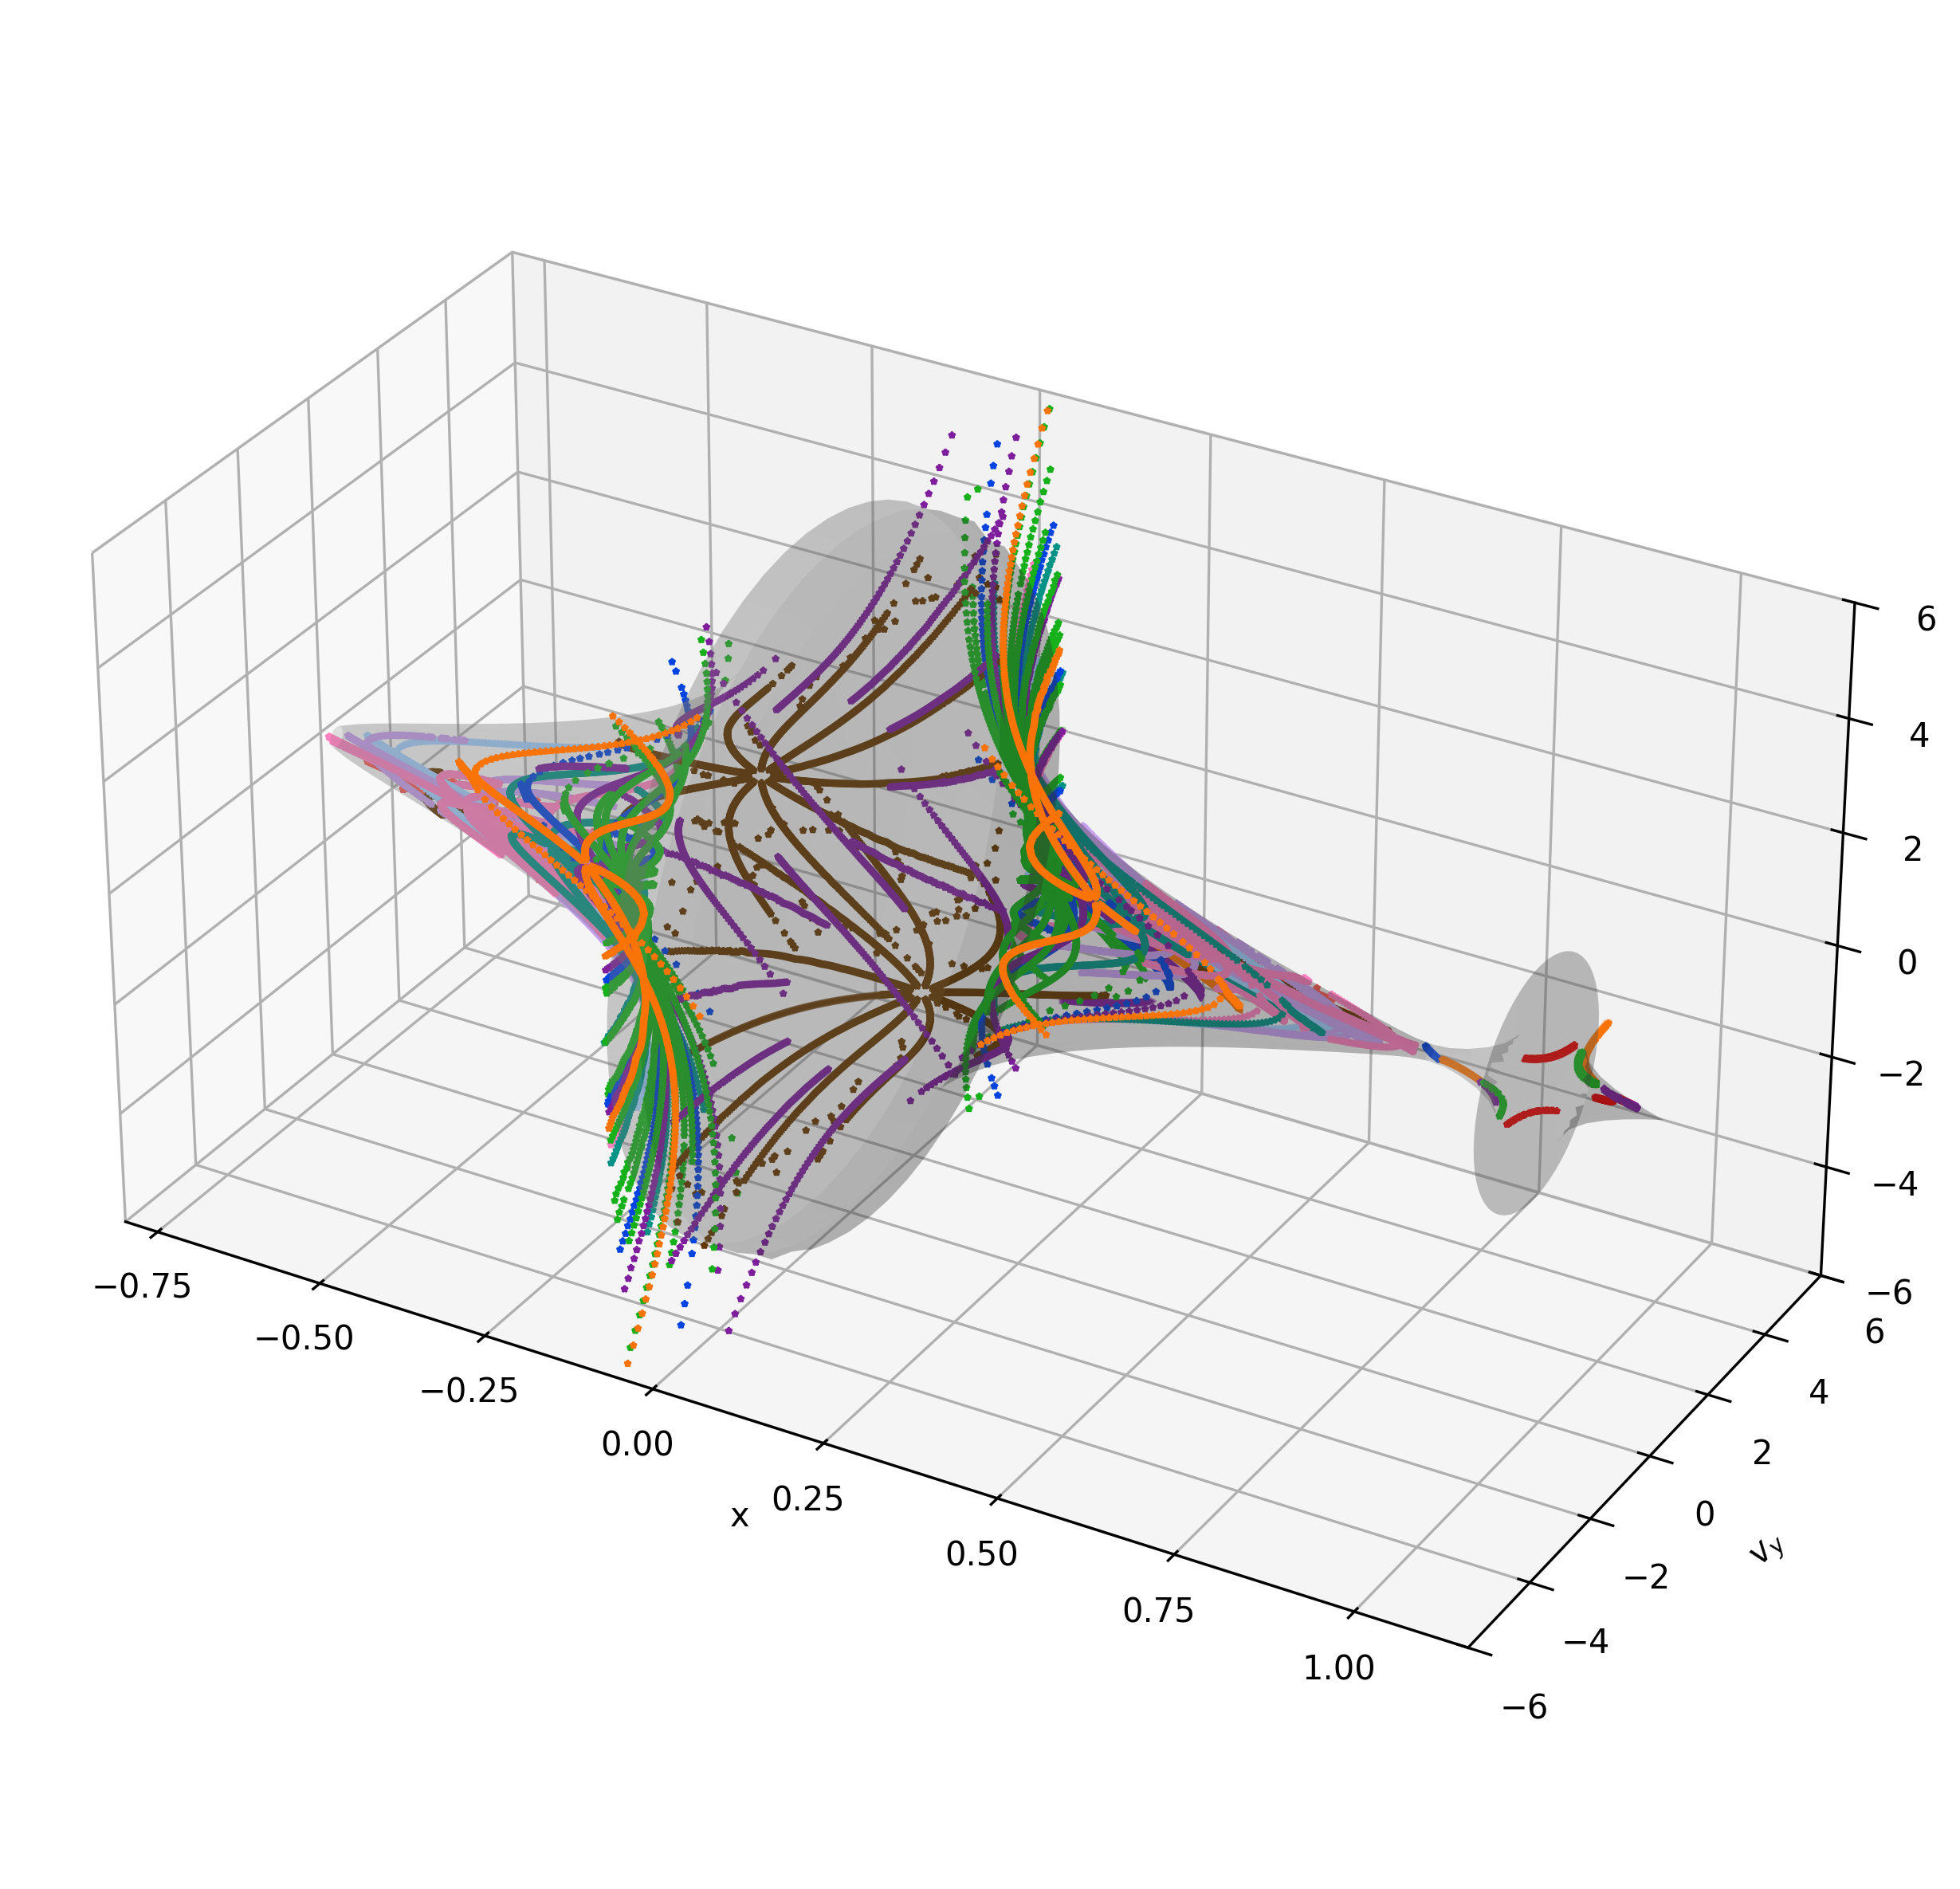
\includegraphics[width=2.9in, trim={1cm 0 0 0}, clip]{images/3D crossings all orbits (without title and legend).png}%
    % %     }%
    % %     % \hfill
    % %     \parbox[c]{3in}{%
    % %         % \centering
    % %         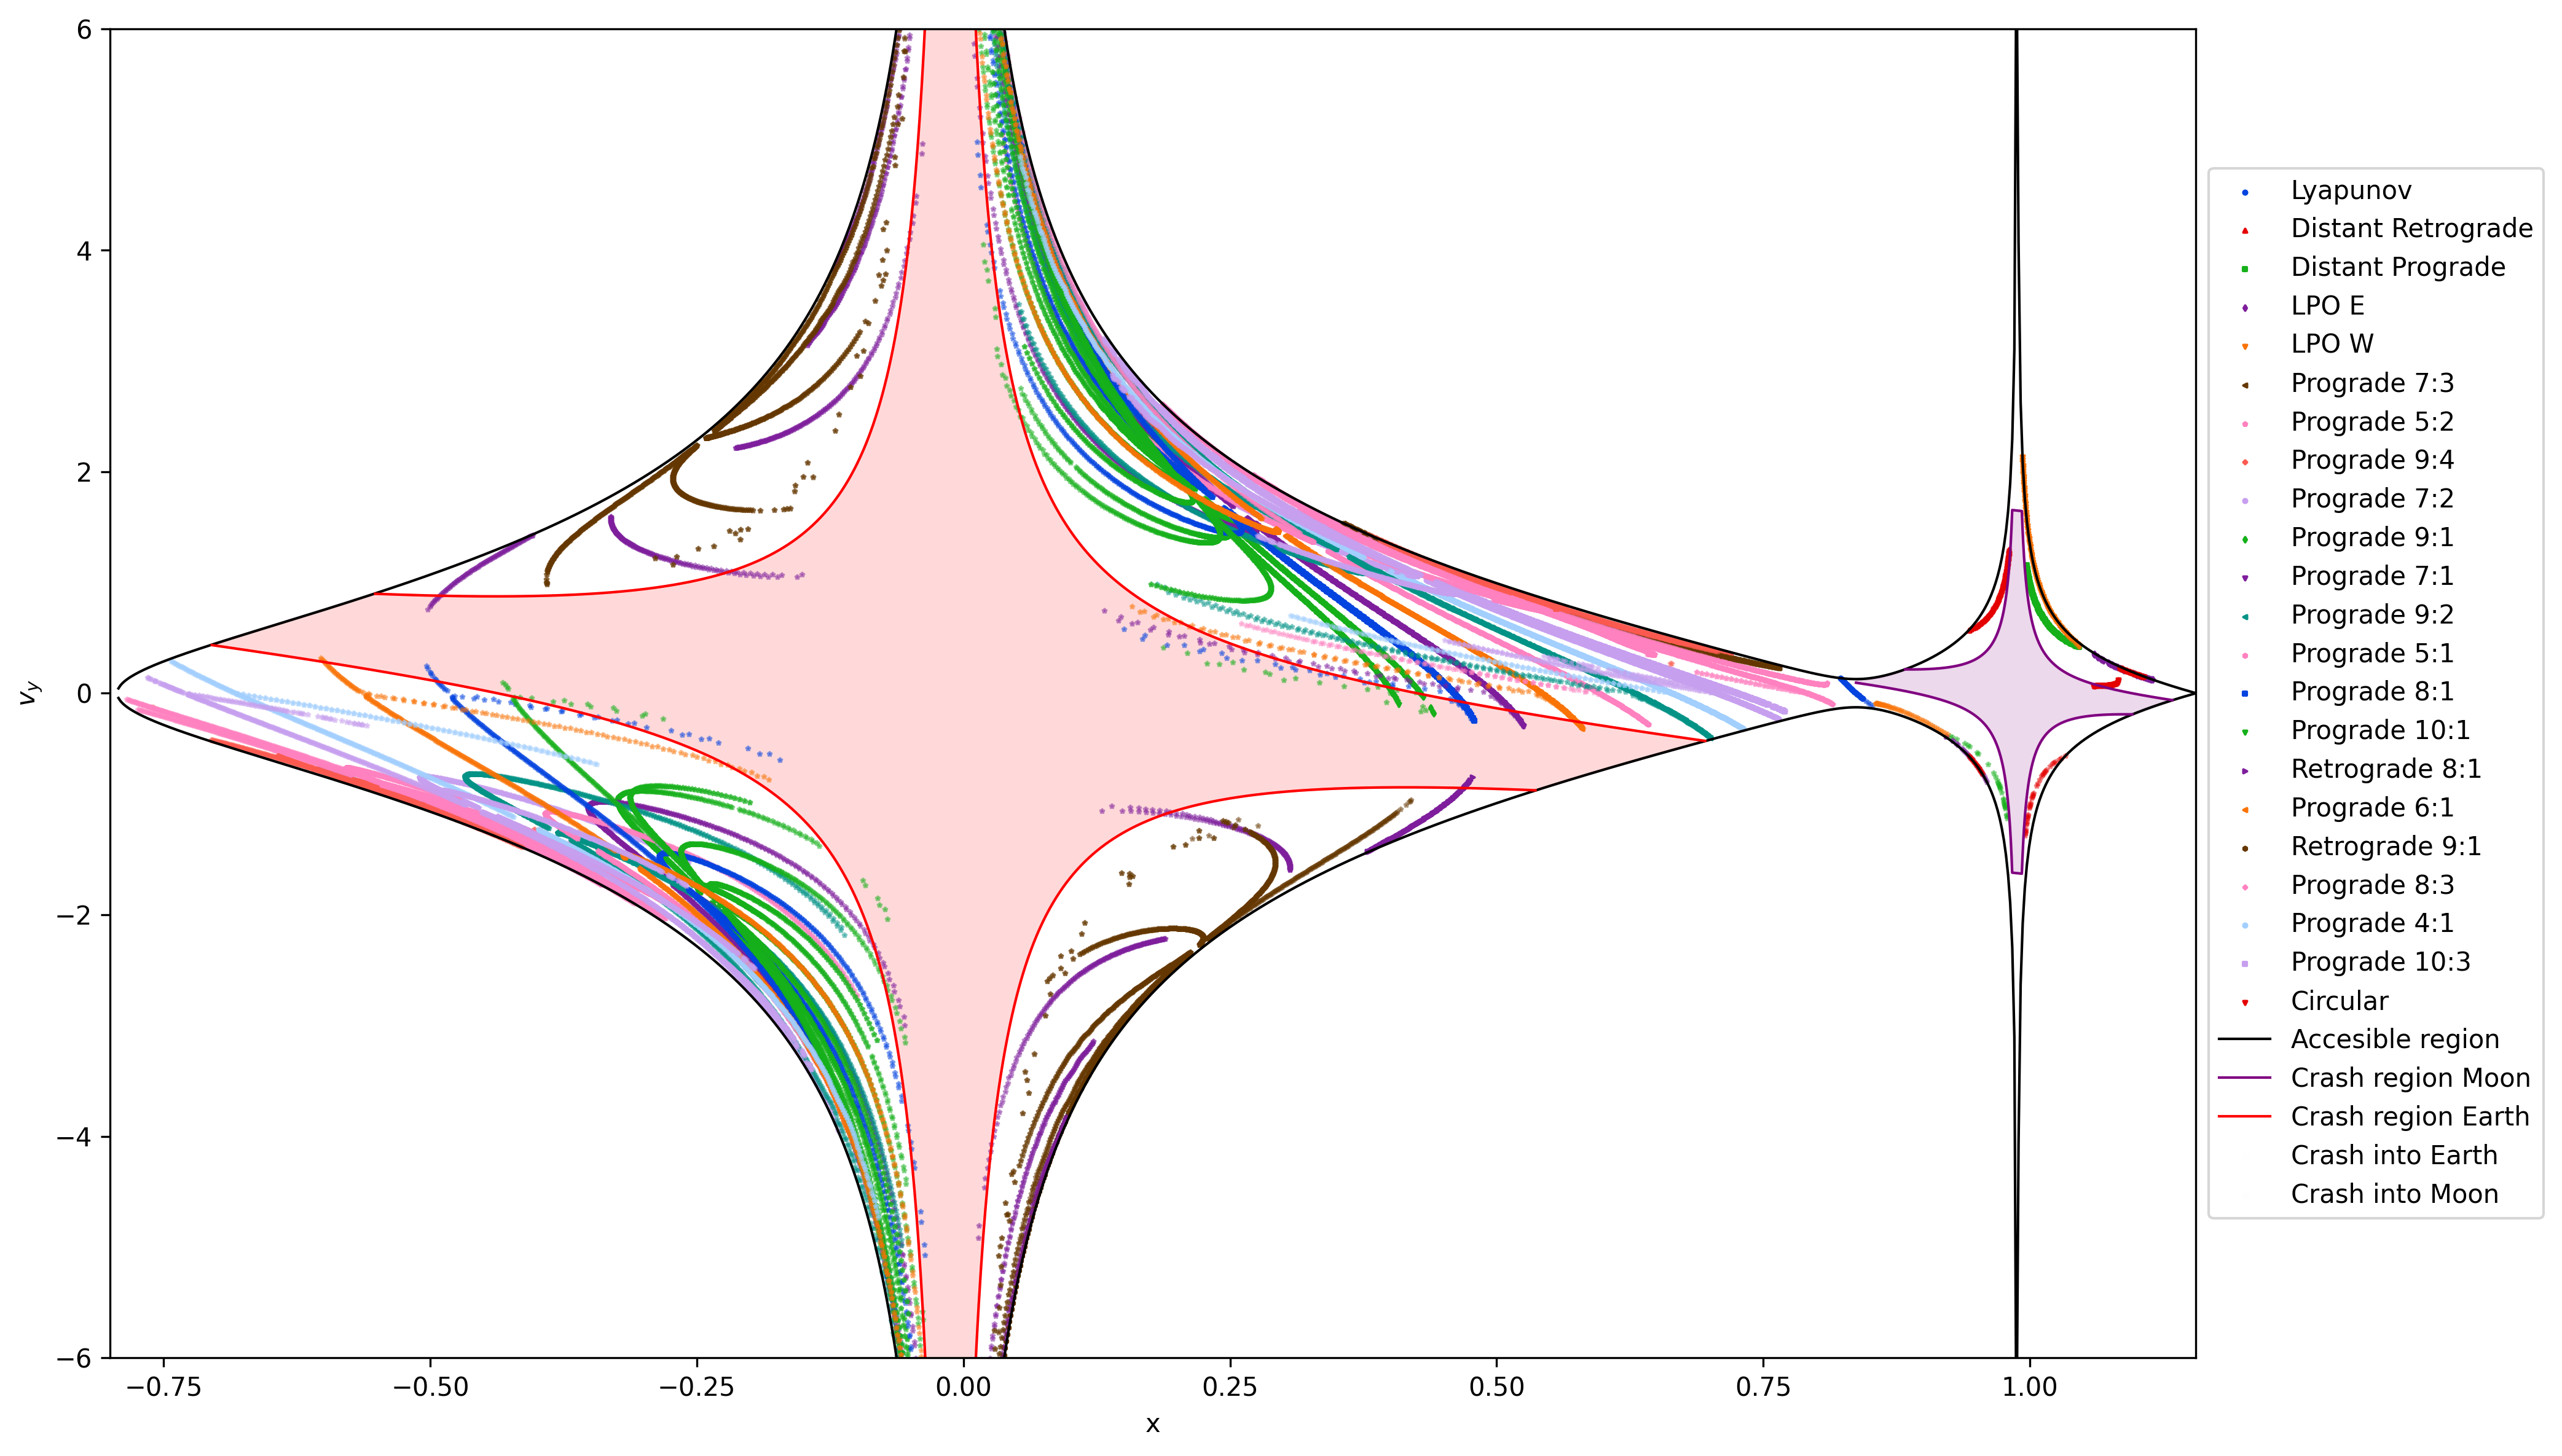
\includegraphics[width=3.5in, trim={0.3cm 0 0 0}, clip]{images/2D crossings all orbits.png}%
    % %     }
    % %     \caption{Visualisations of the accessible region in three dimensions and its projection to the $(x,v_y)$ plane, displaying the Earth and Moon crash regions.}
    % %     \label{fig:accesible region 3D and 2D}
    % % \end{figure}
        

% \newpage %temporarily




\section{Simulations and Results} \label{sec:Simulation Results}



\subsection{Orbital Crossings} \label{subsec:Orbital Crossings}



        
    


    Following the process laid out in \cref{subsec: computationOfPlanarResonantOrbits} to compute the crossings of planar resonant orbits, code employing the use of pydylan (a Python interface to the Dynamically Leveraged Automated (N) Multibody Trajectory Optimization software, \cite{beeson2022dynamically}) was written to plot these crossings within the accessible region for several different orbital families.


    \begin{figure}[ht] \label{fig:orbital crossings plotted}
    	\centering
        % 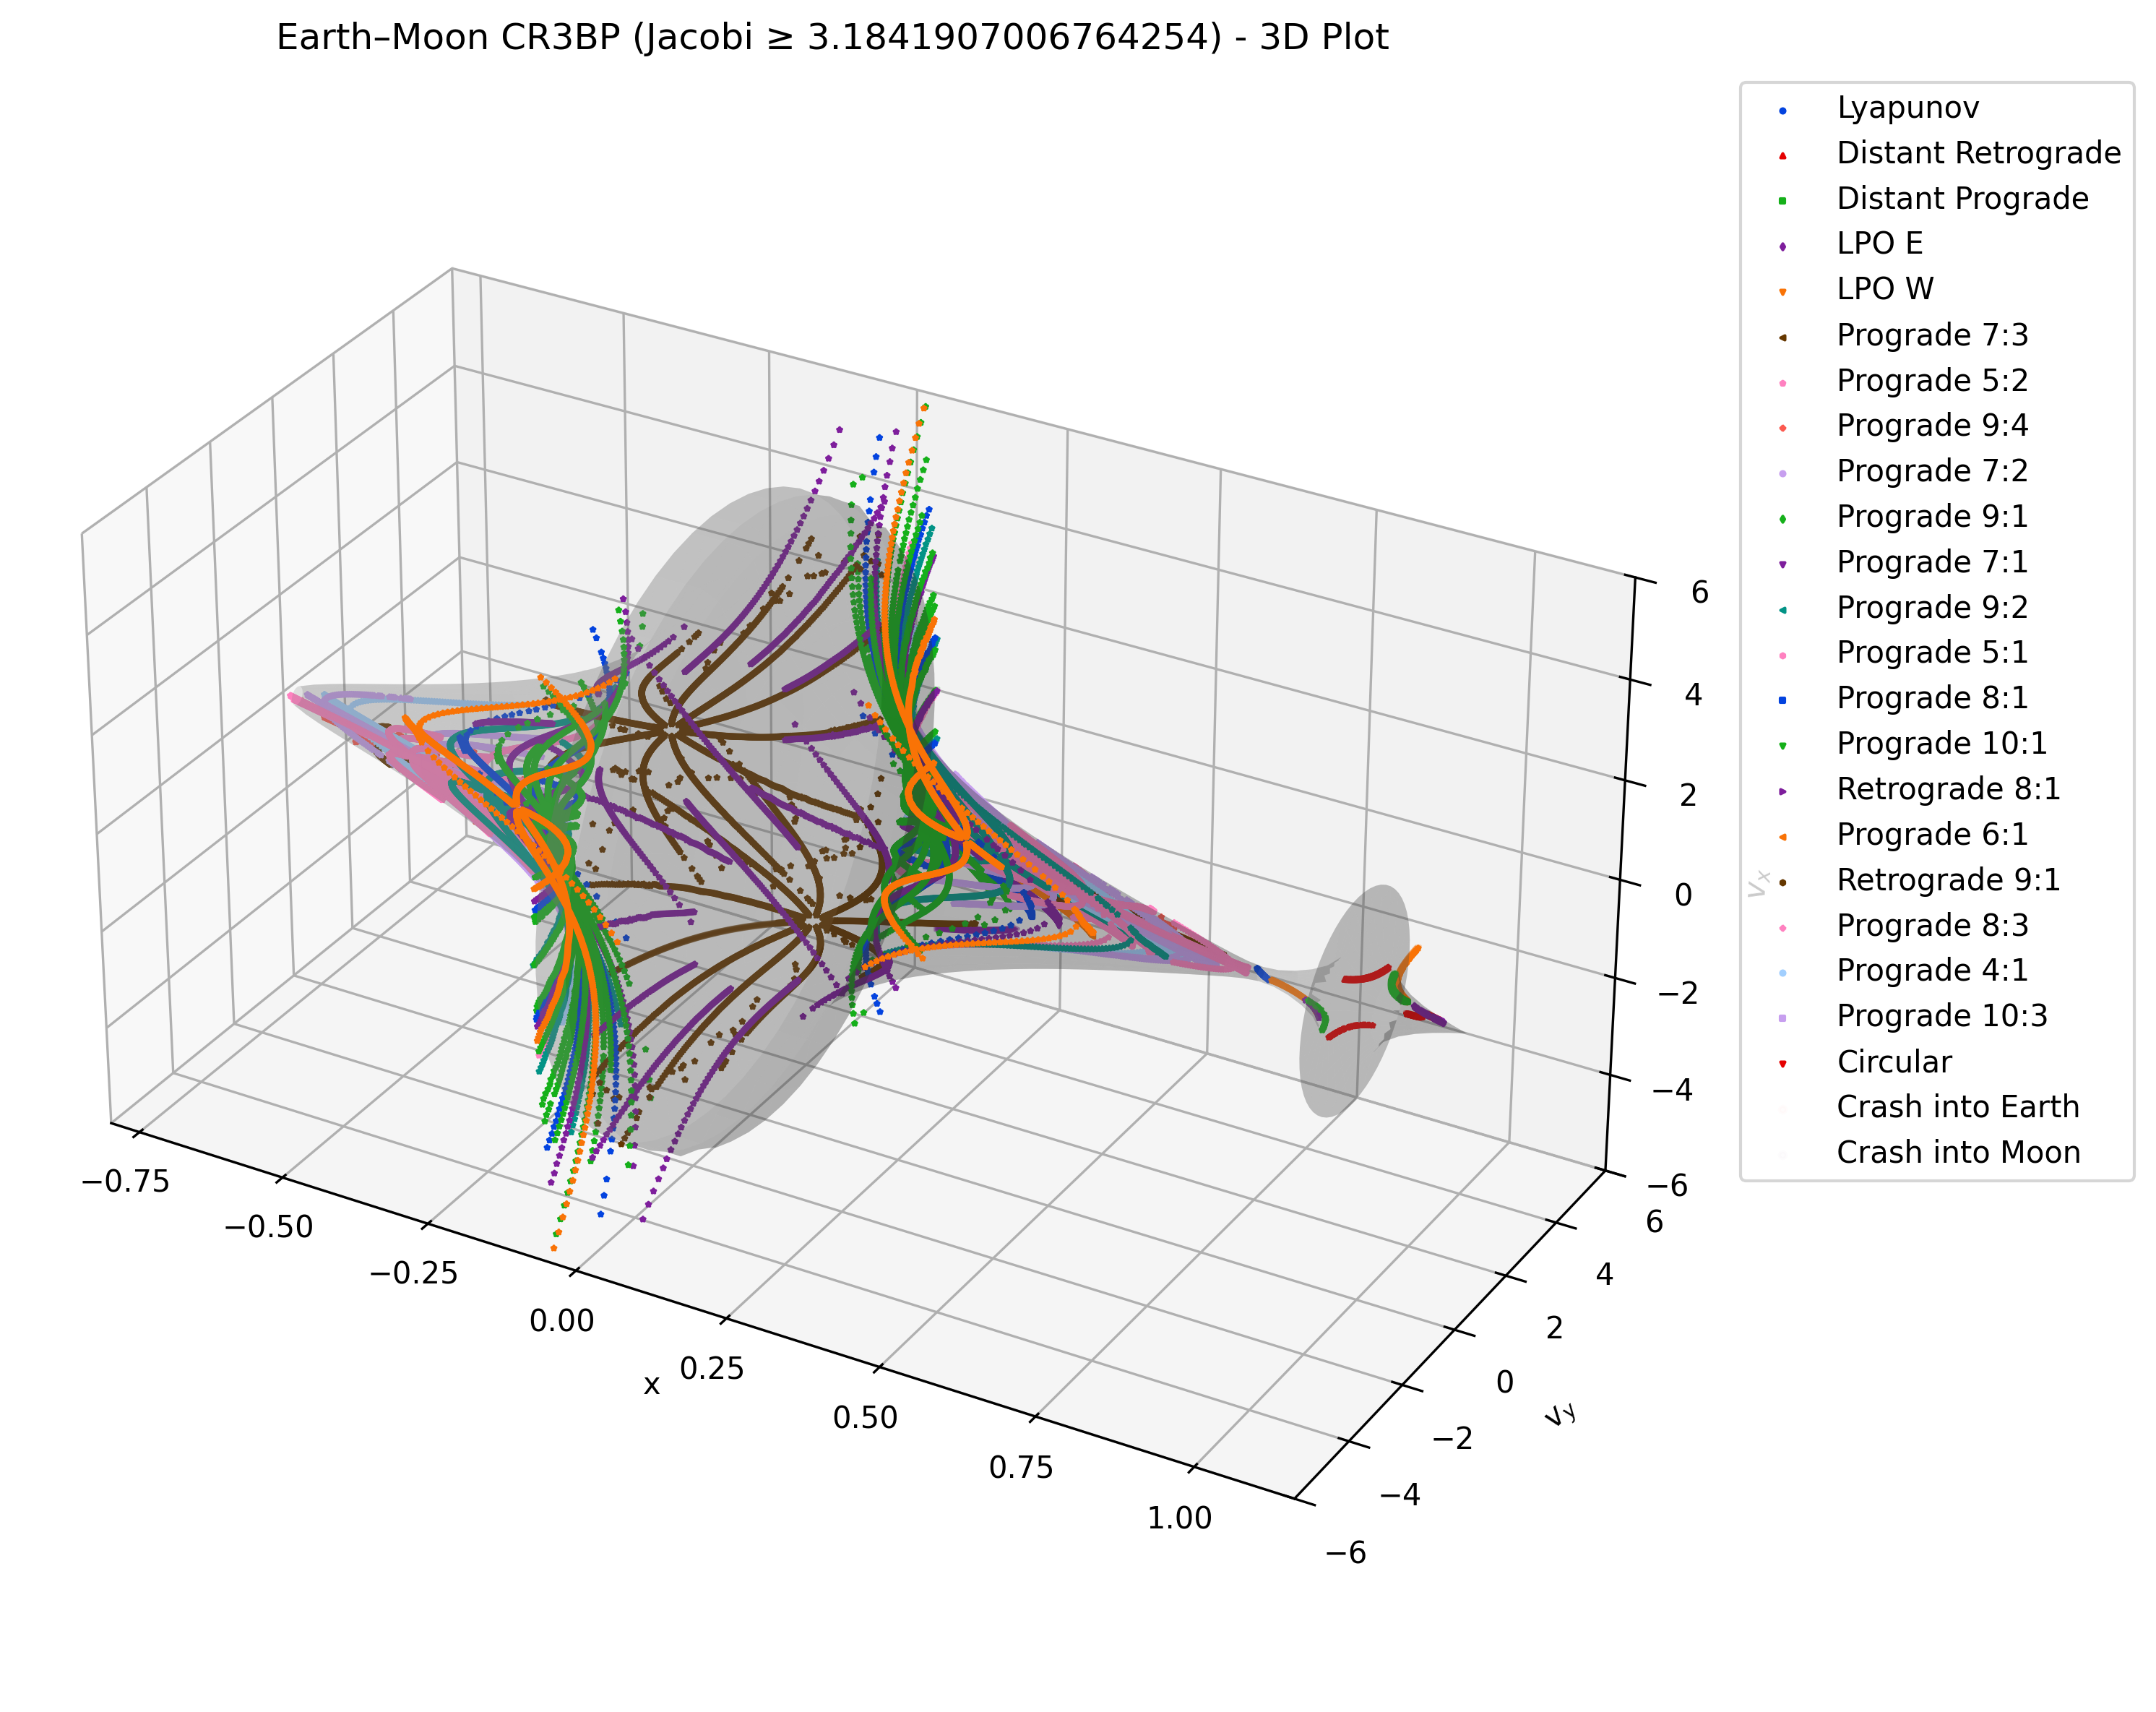
\includegraphics[width=2.9in]{images/3D crossings all orbits.png}
        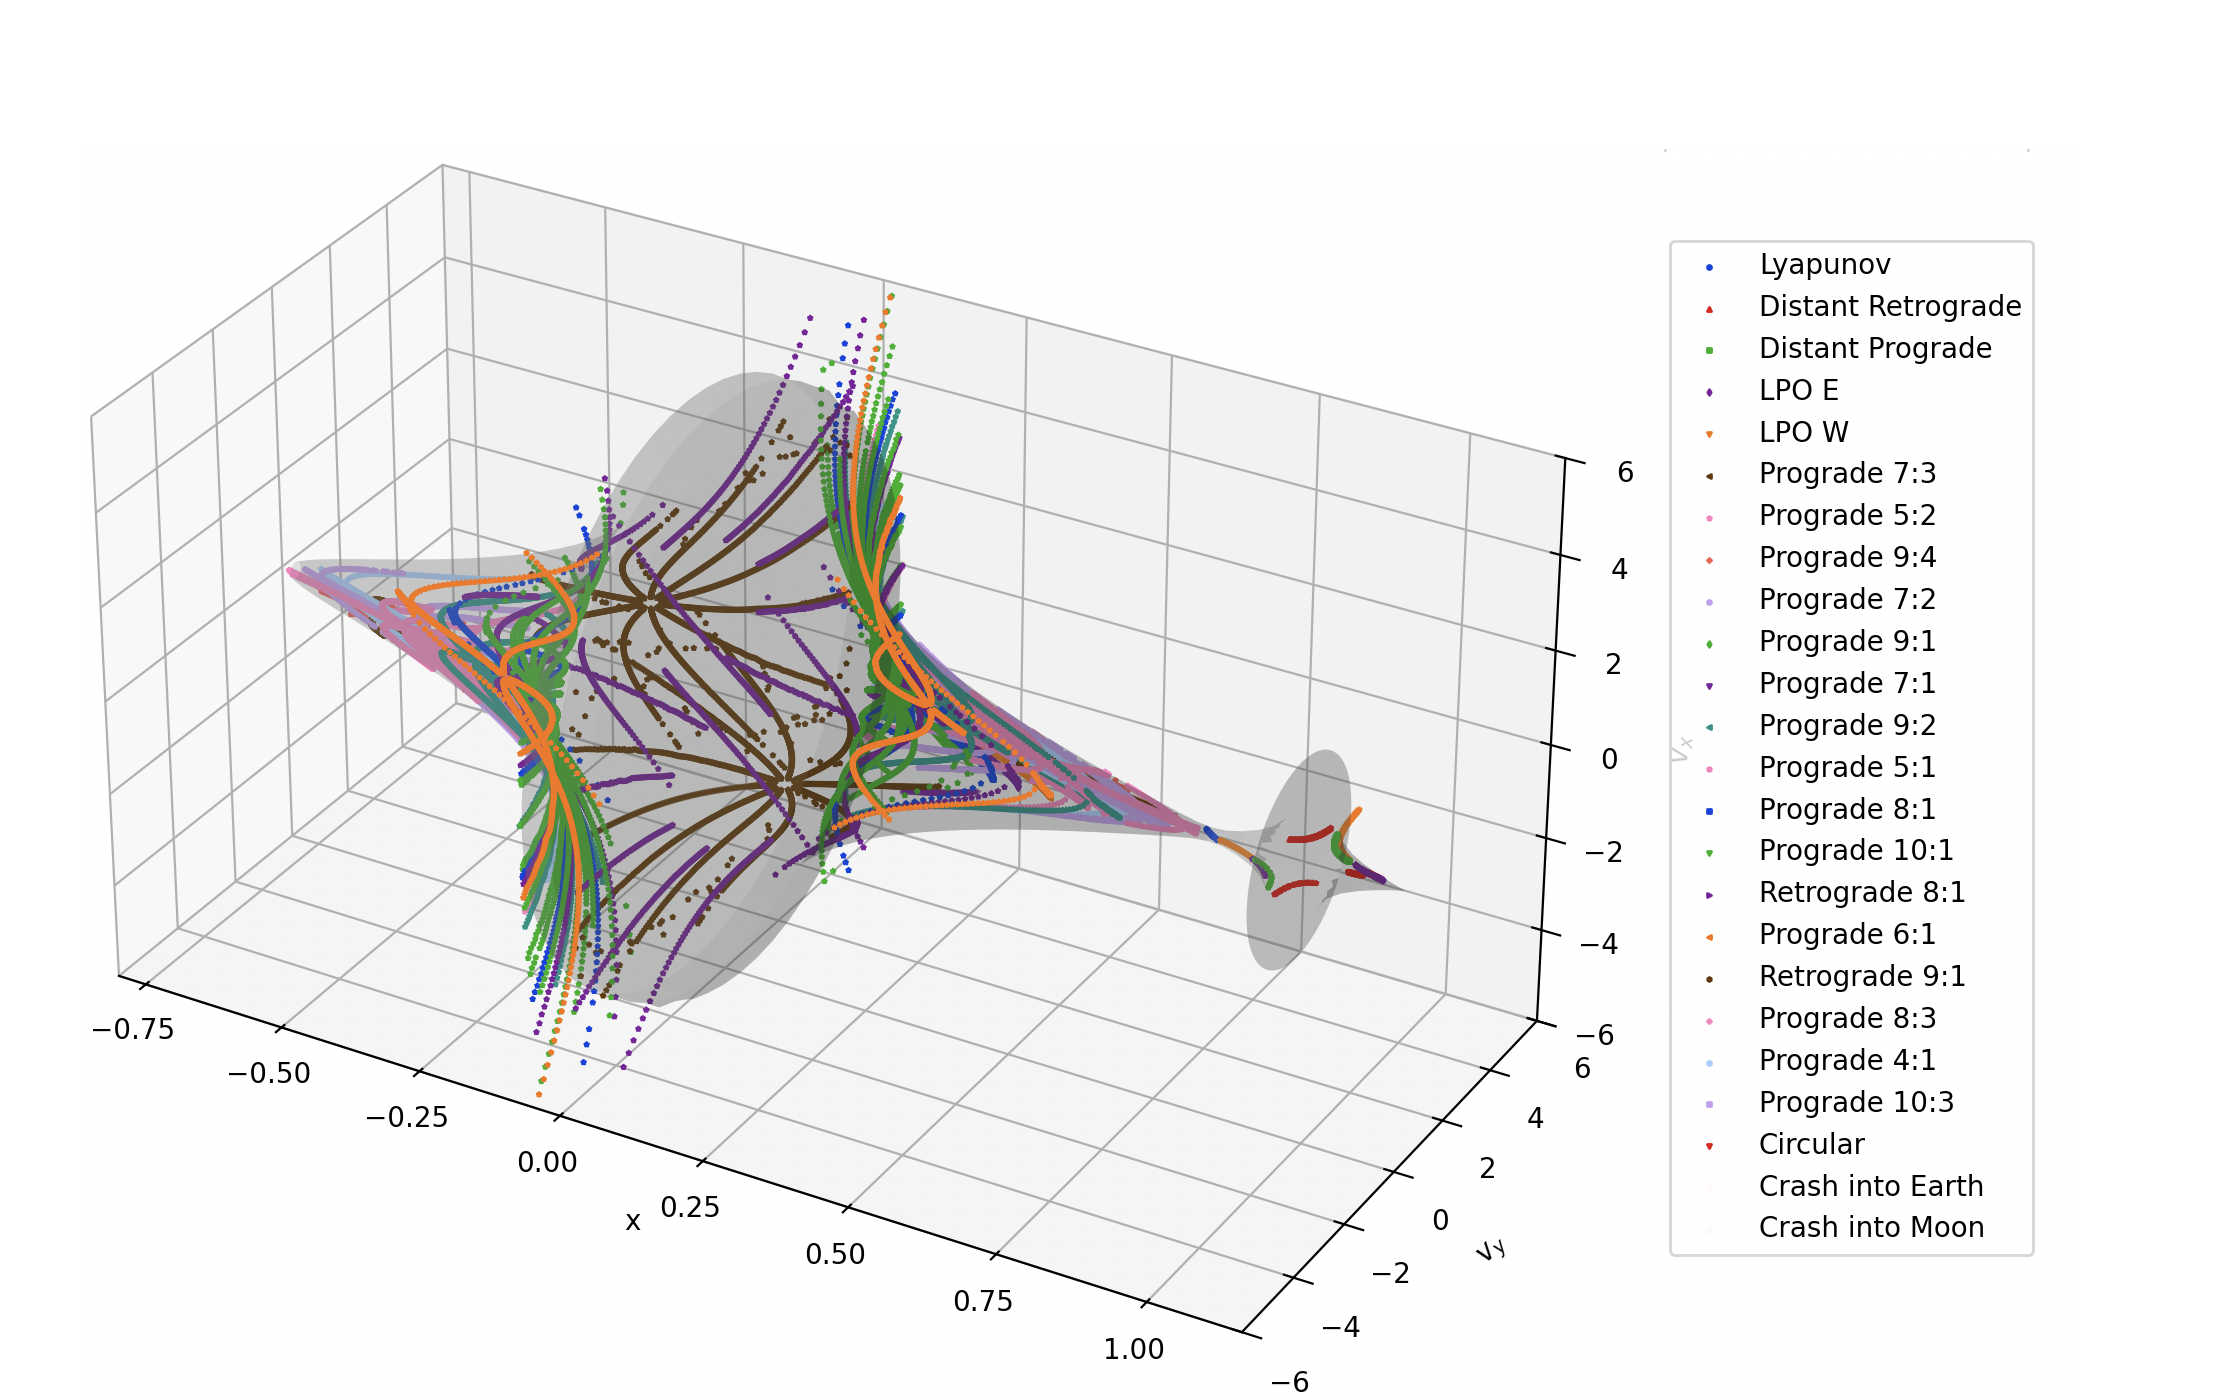
\includegraphics[width=0.85\linewidth]{images/manually made 3d.png}
        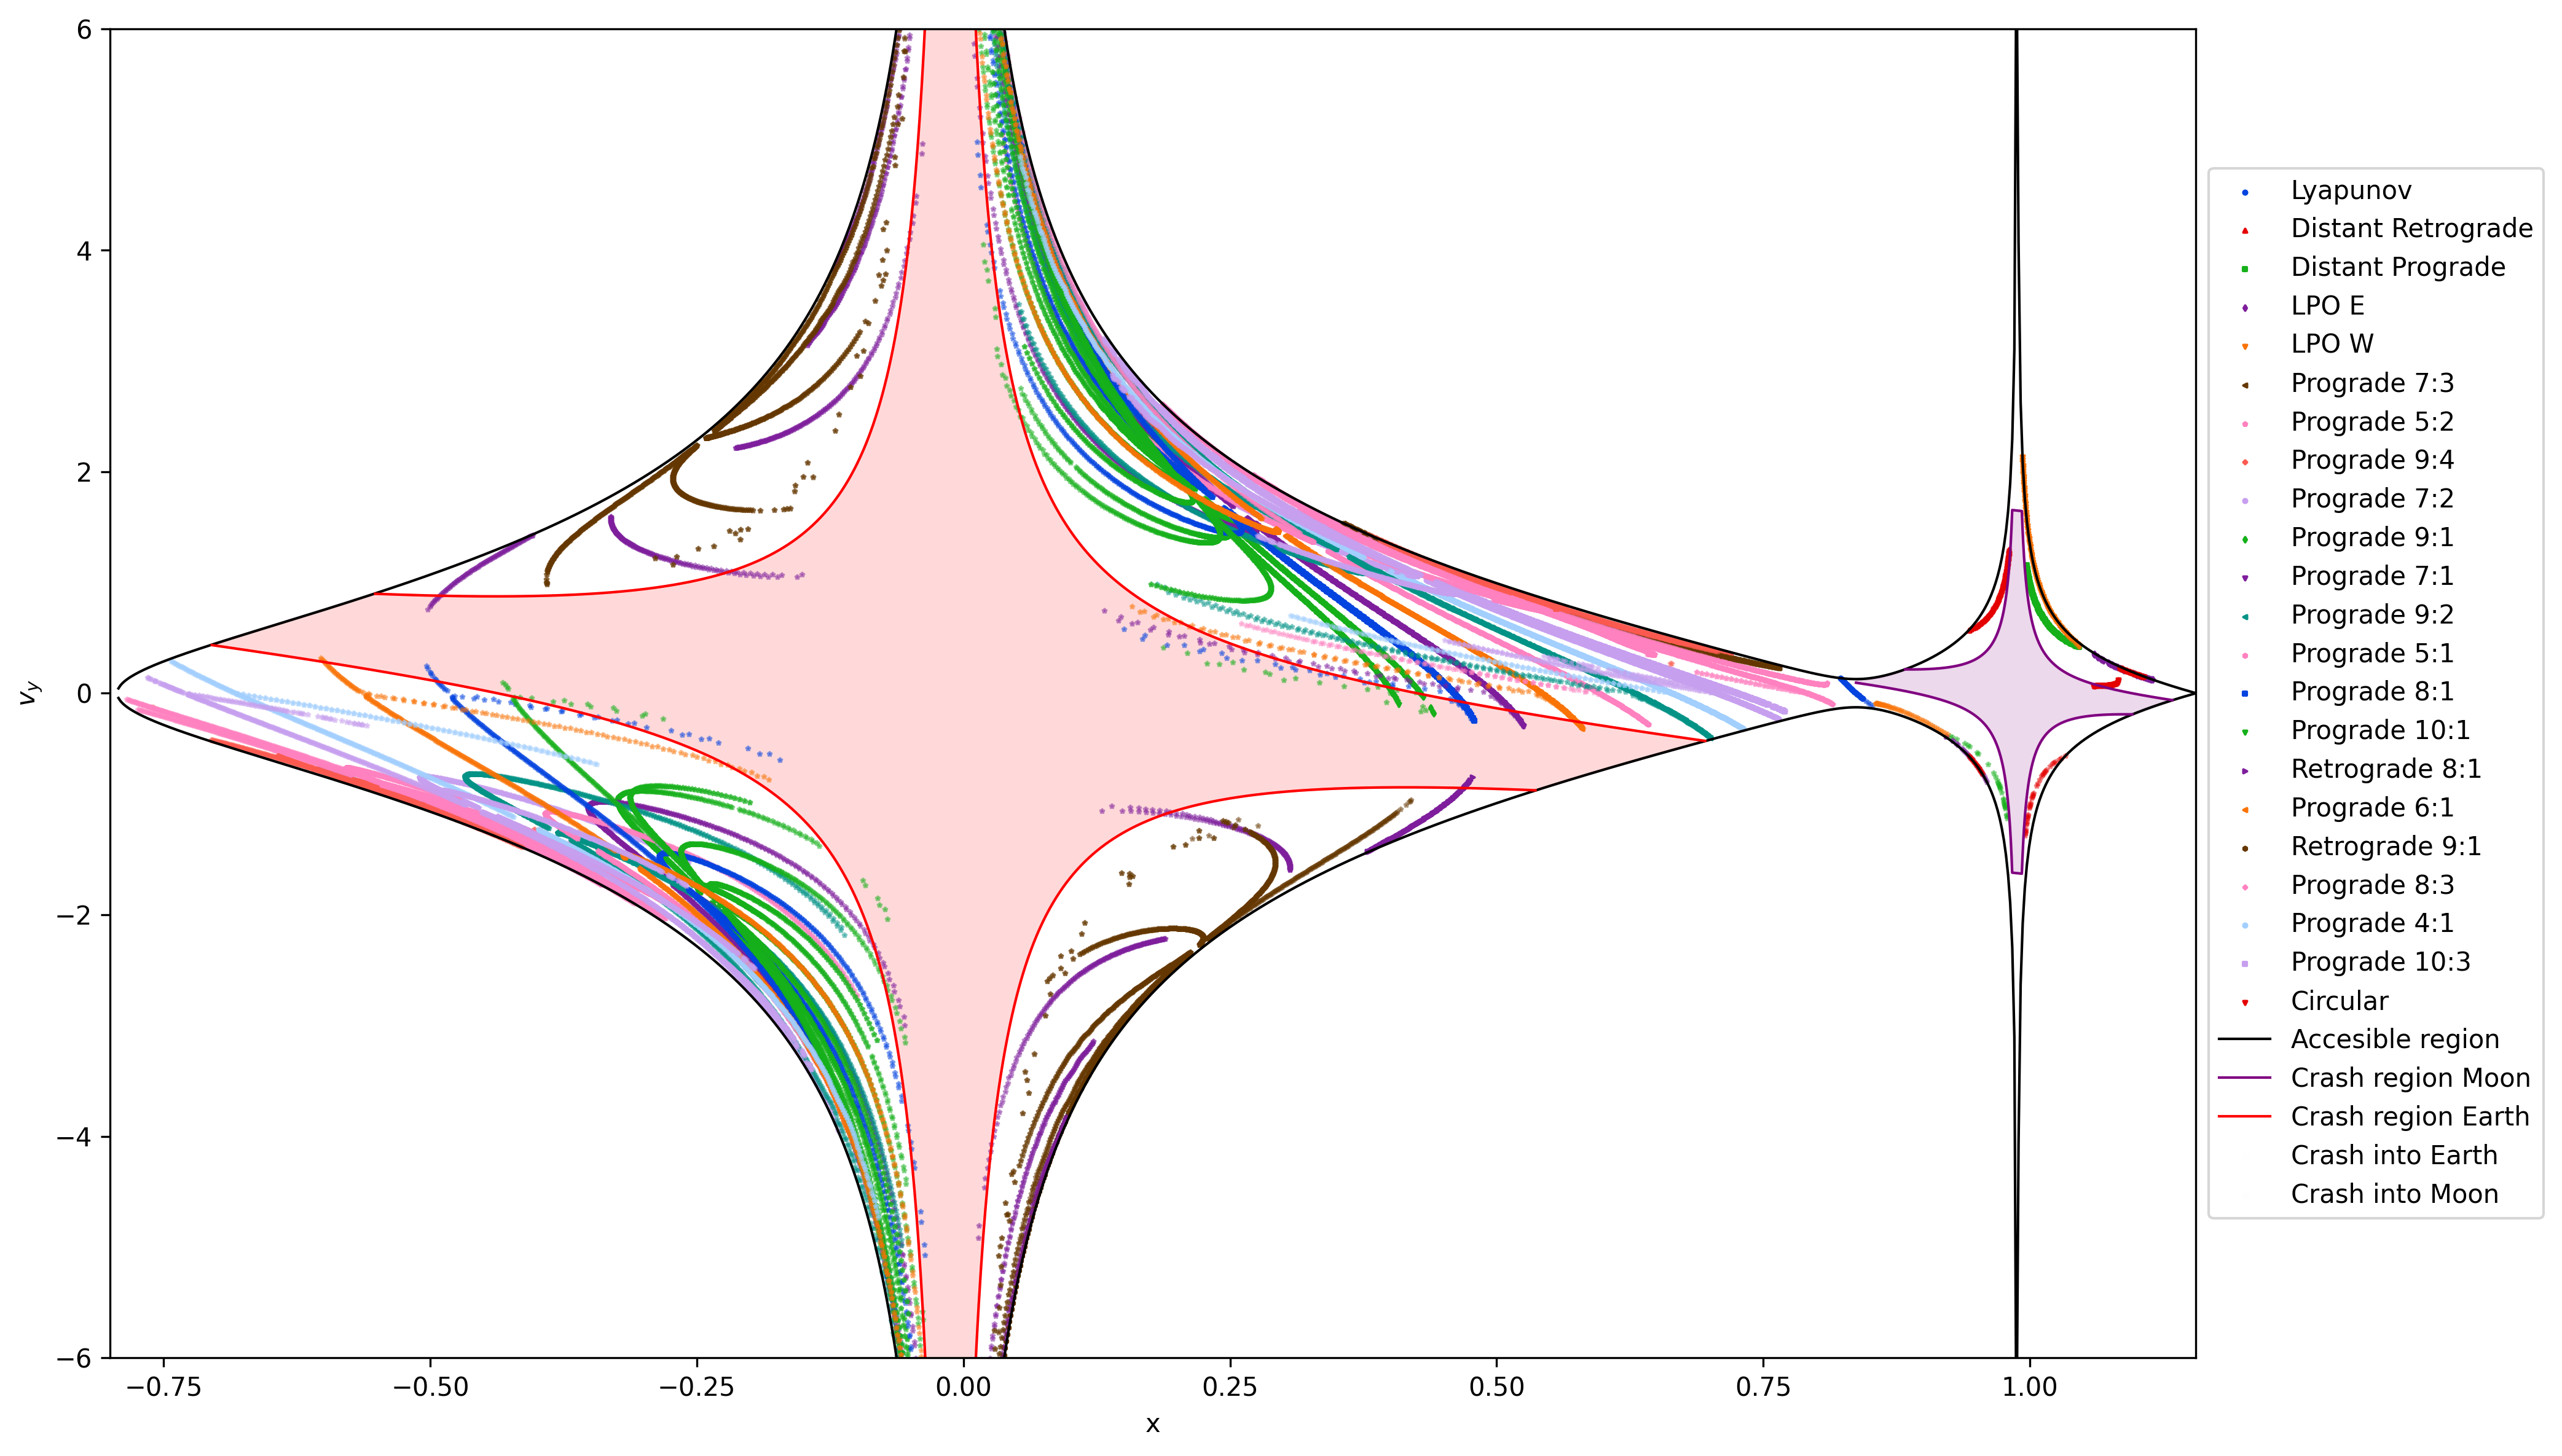
\includegraphics[width=0.75\linewidth]{images/2D crossings all orbits.png}
        % \caption{Visualisations of the accessible region in three dimensions and its projection to the $(x,v_y)$ plane, displaying the Earth and Moon crash regions. The larger `pseudosphere'-esque region corresponds to the region around Earth, and the smaller: that of the Moon.}
        \caption{Orbital crossings of several planar resonant orbits, depicted in three-dimensions and the projection to the $(x,v_y)$ plane.}
        \label{fig: crossings}
    \end{figure}


    

    In \cref{fig: crossings}, these crossings are depicted in the three-dimensional $x,v_x,v_y$ space, as well as in the projection down to the $x,v_y$ plane, for visual clarity. The colours specified in the legend are consistent across both plots. Although it appears as though some points enter the Earth crash region in the 2D image, this is simply a consequence/limitation of the use of projection.
    
    


    
    % \begin{figure}[hb] \label{fig:orbital crossings plotted}
    % 	\centering
    %     % 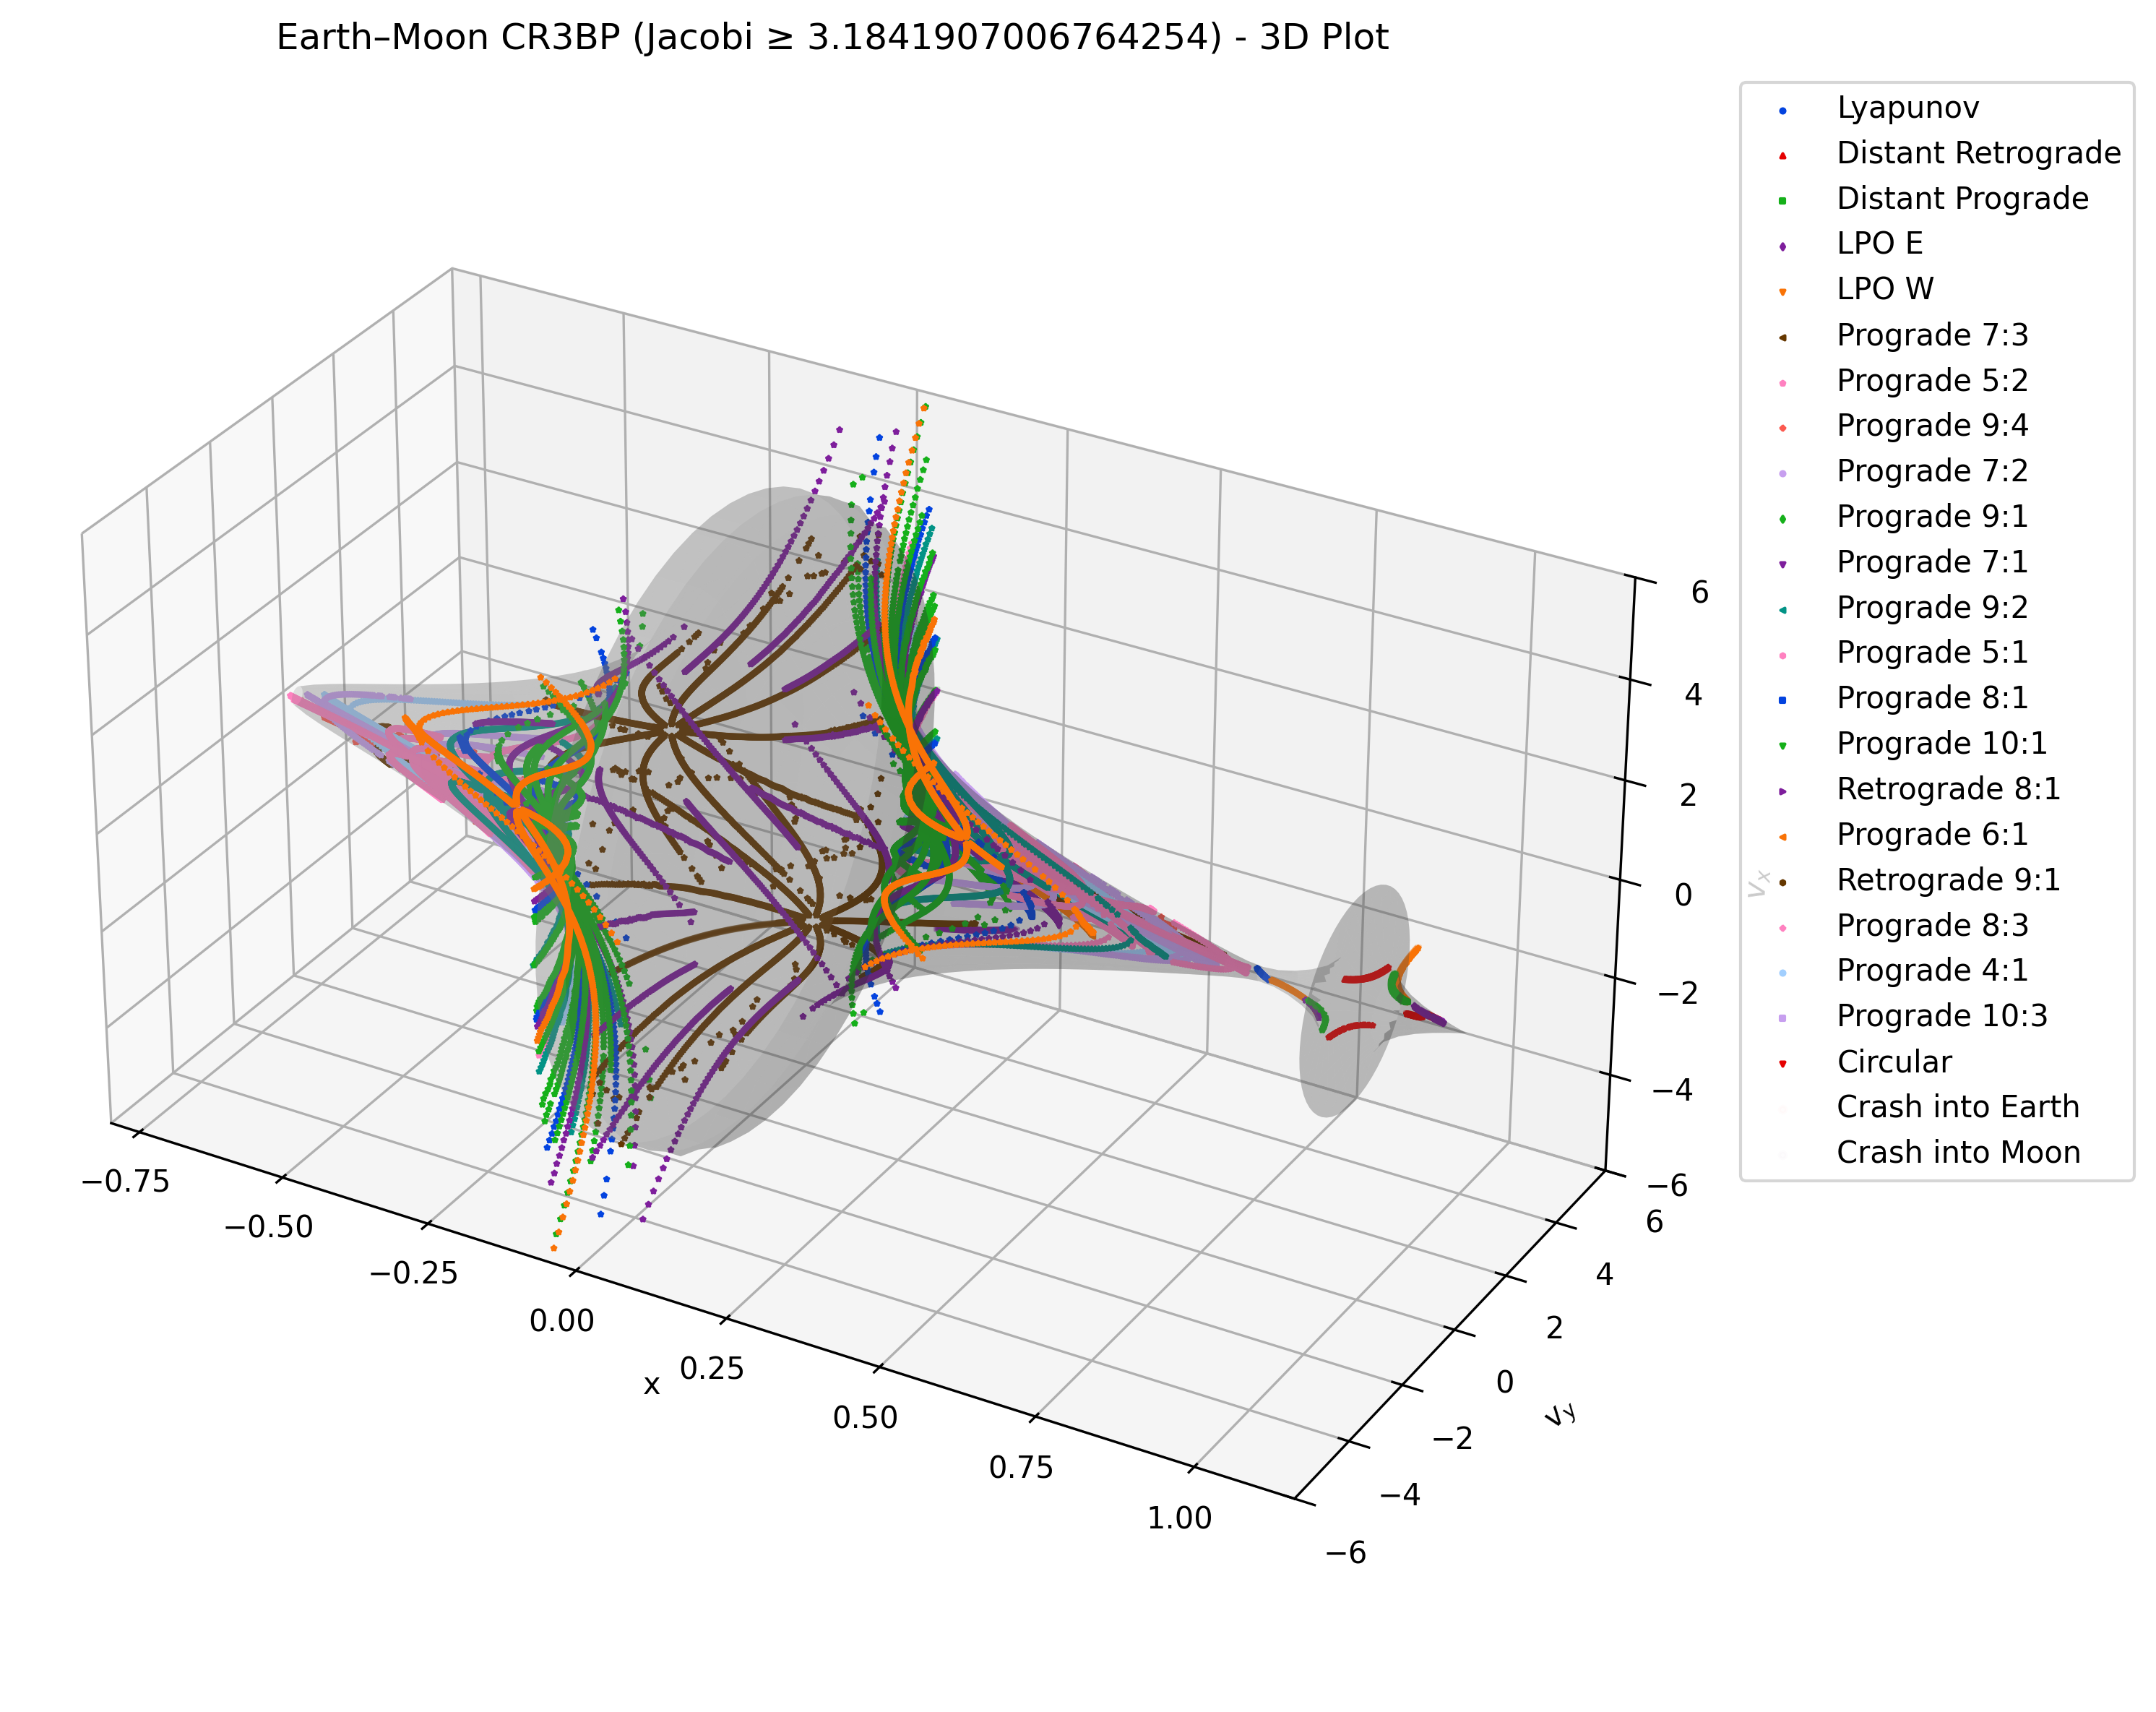
\includegraphics[width=2.9in]{images/3D crossings all orbits.png}
    %     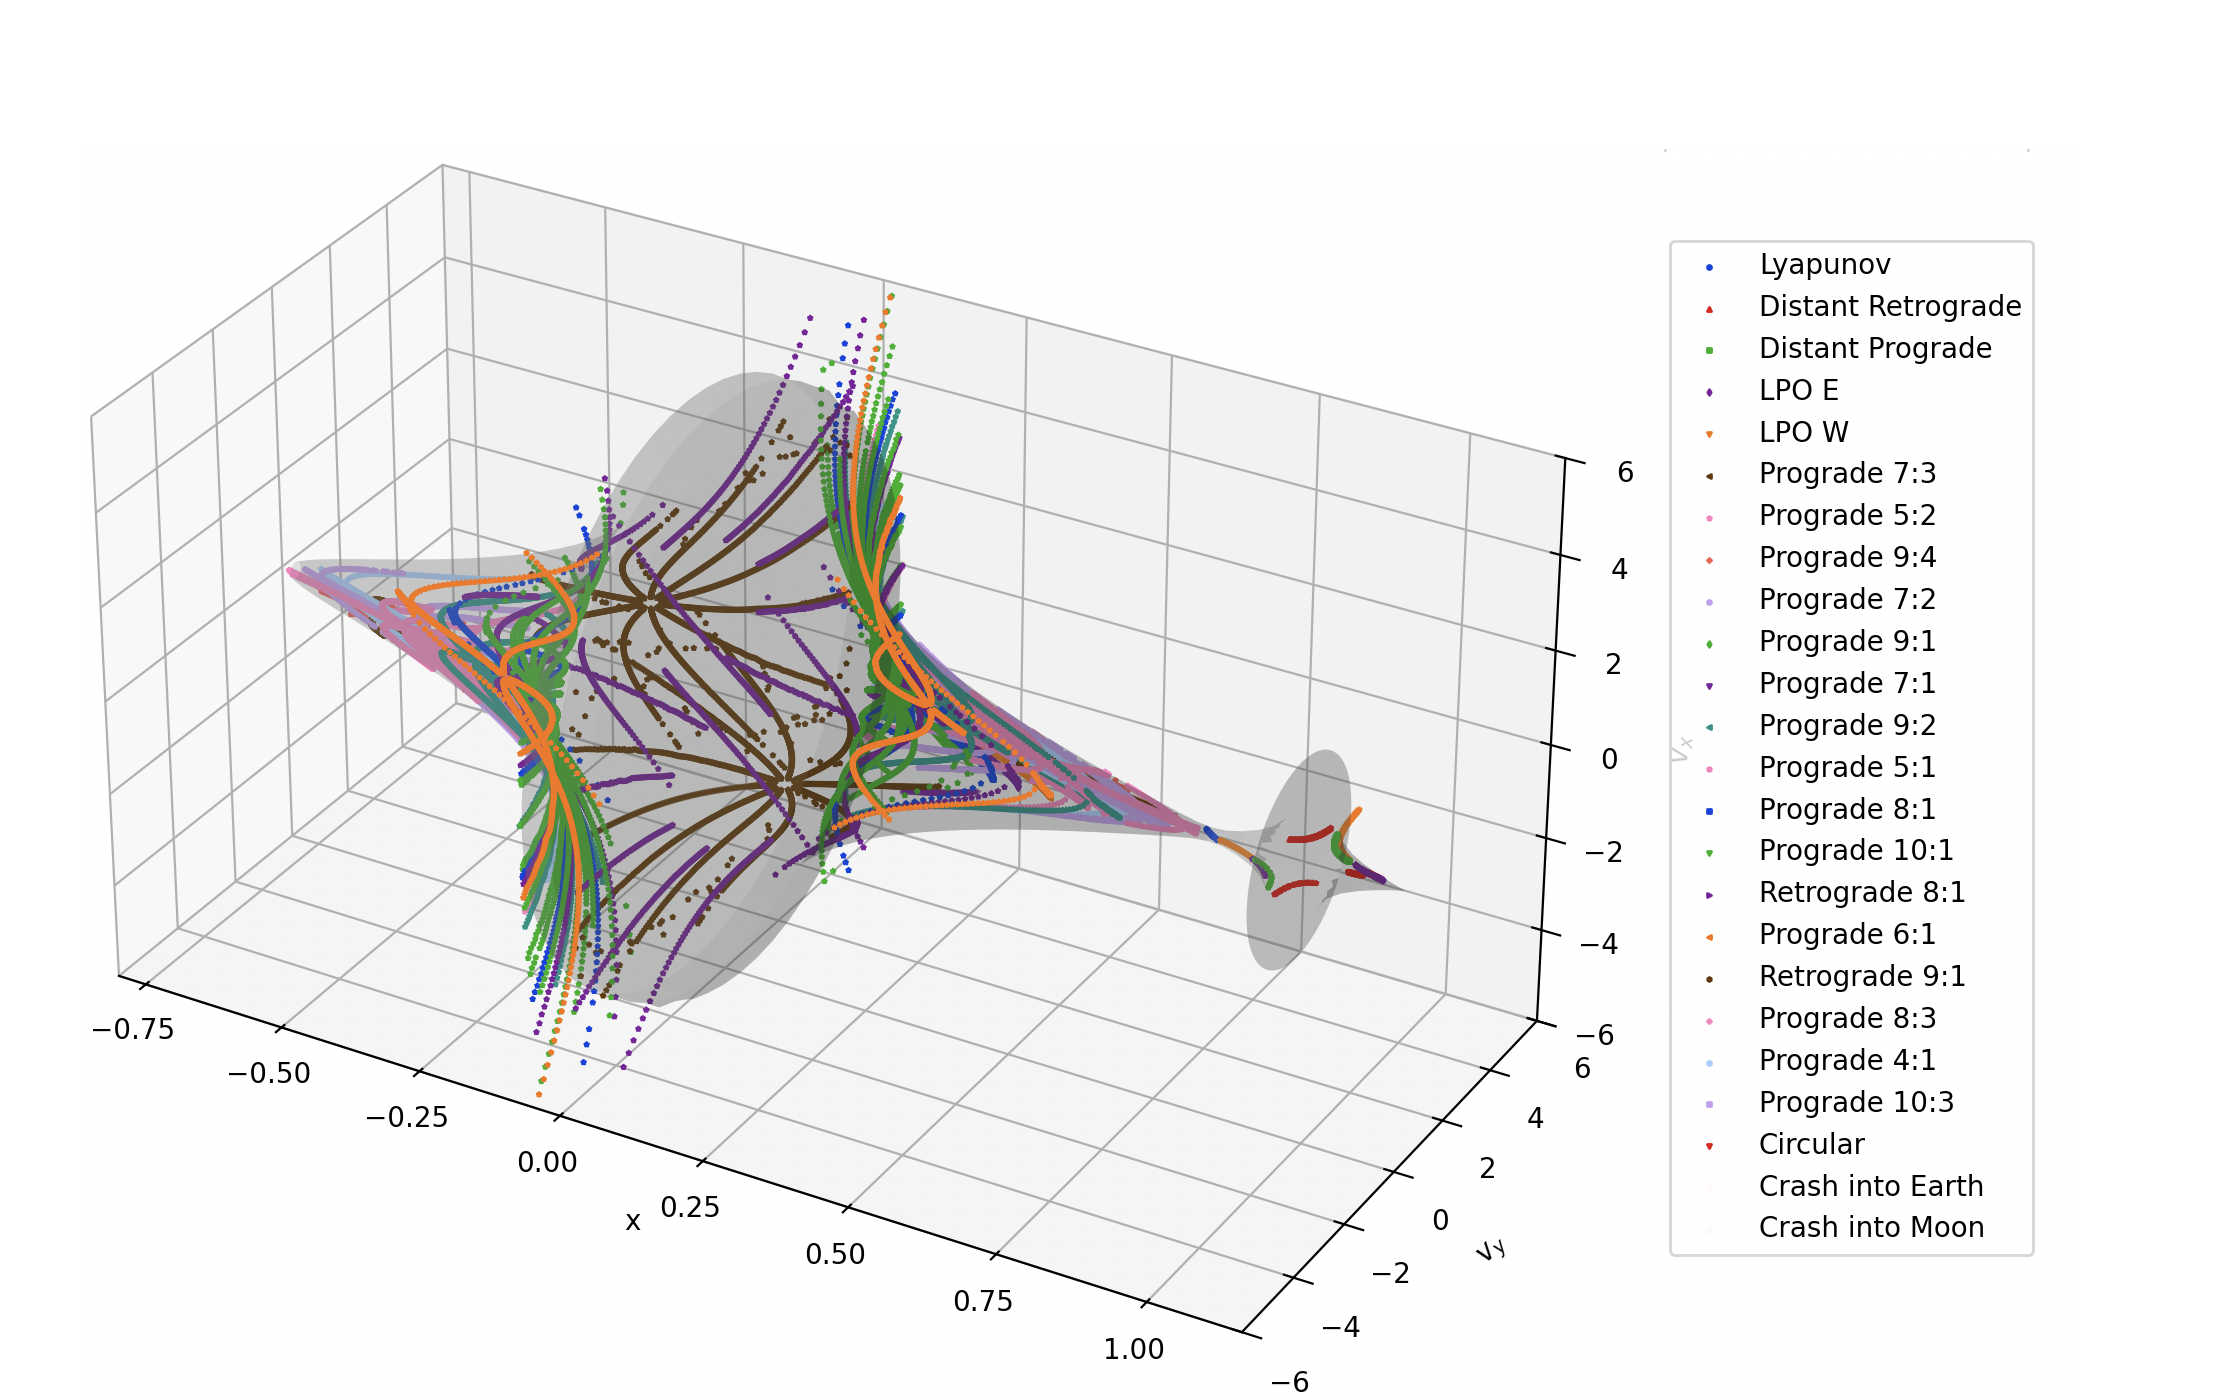
\includegraphics[width=0.85\linewidth]{images/manually made 3d.png}
    %     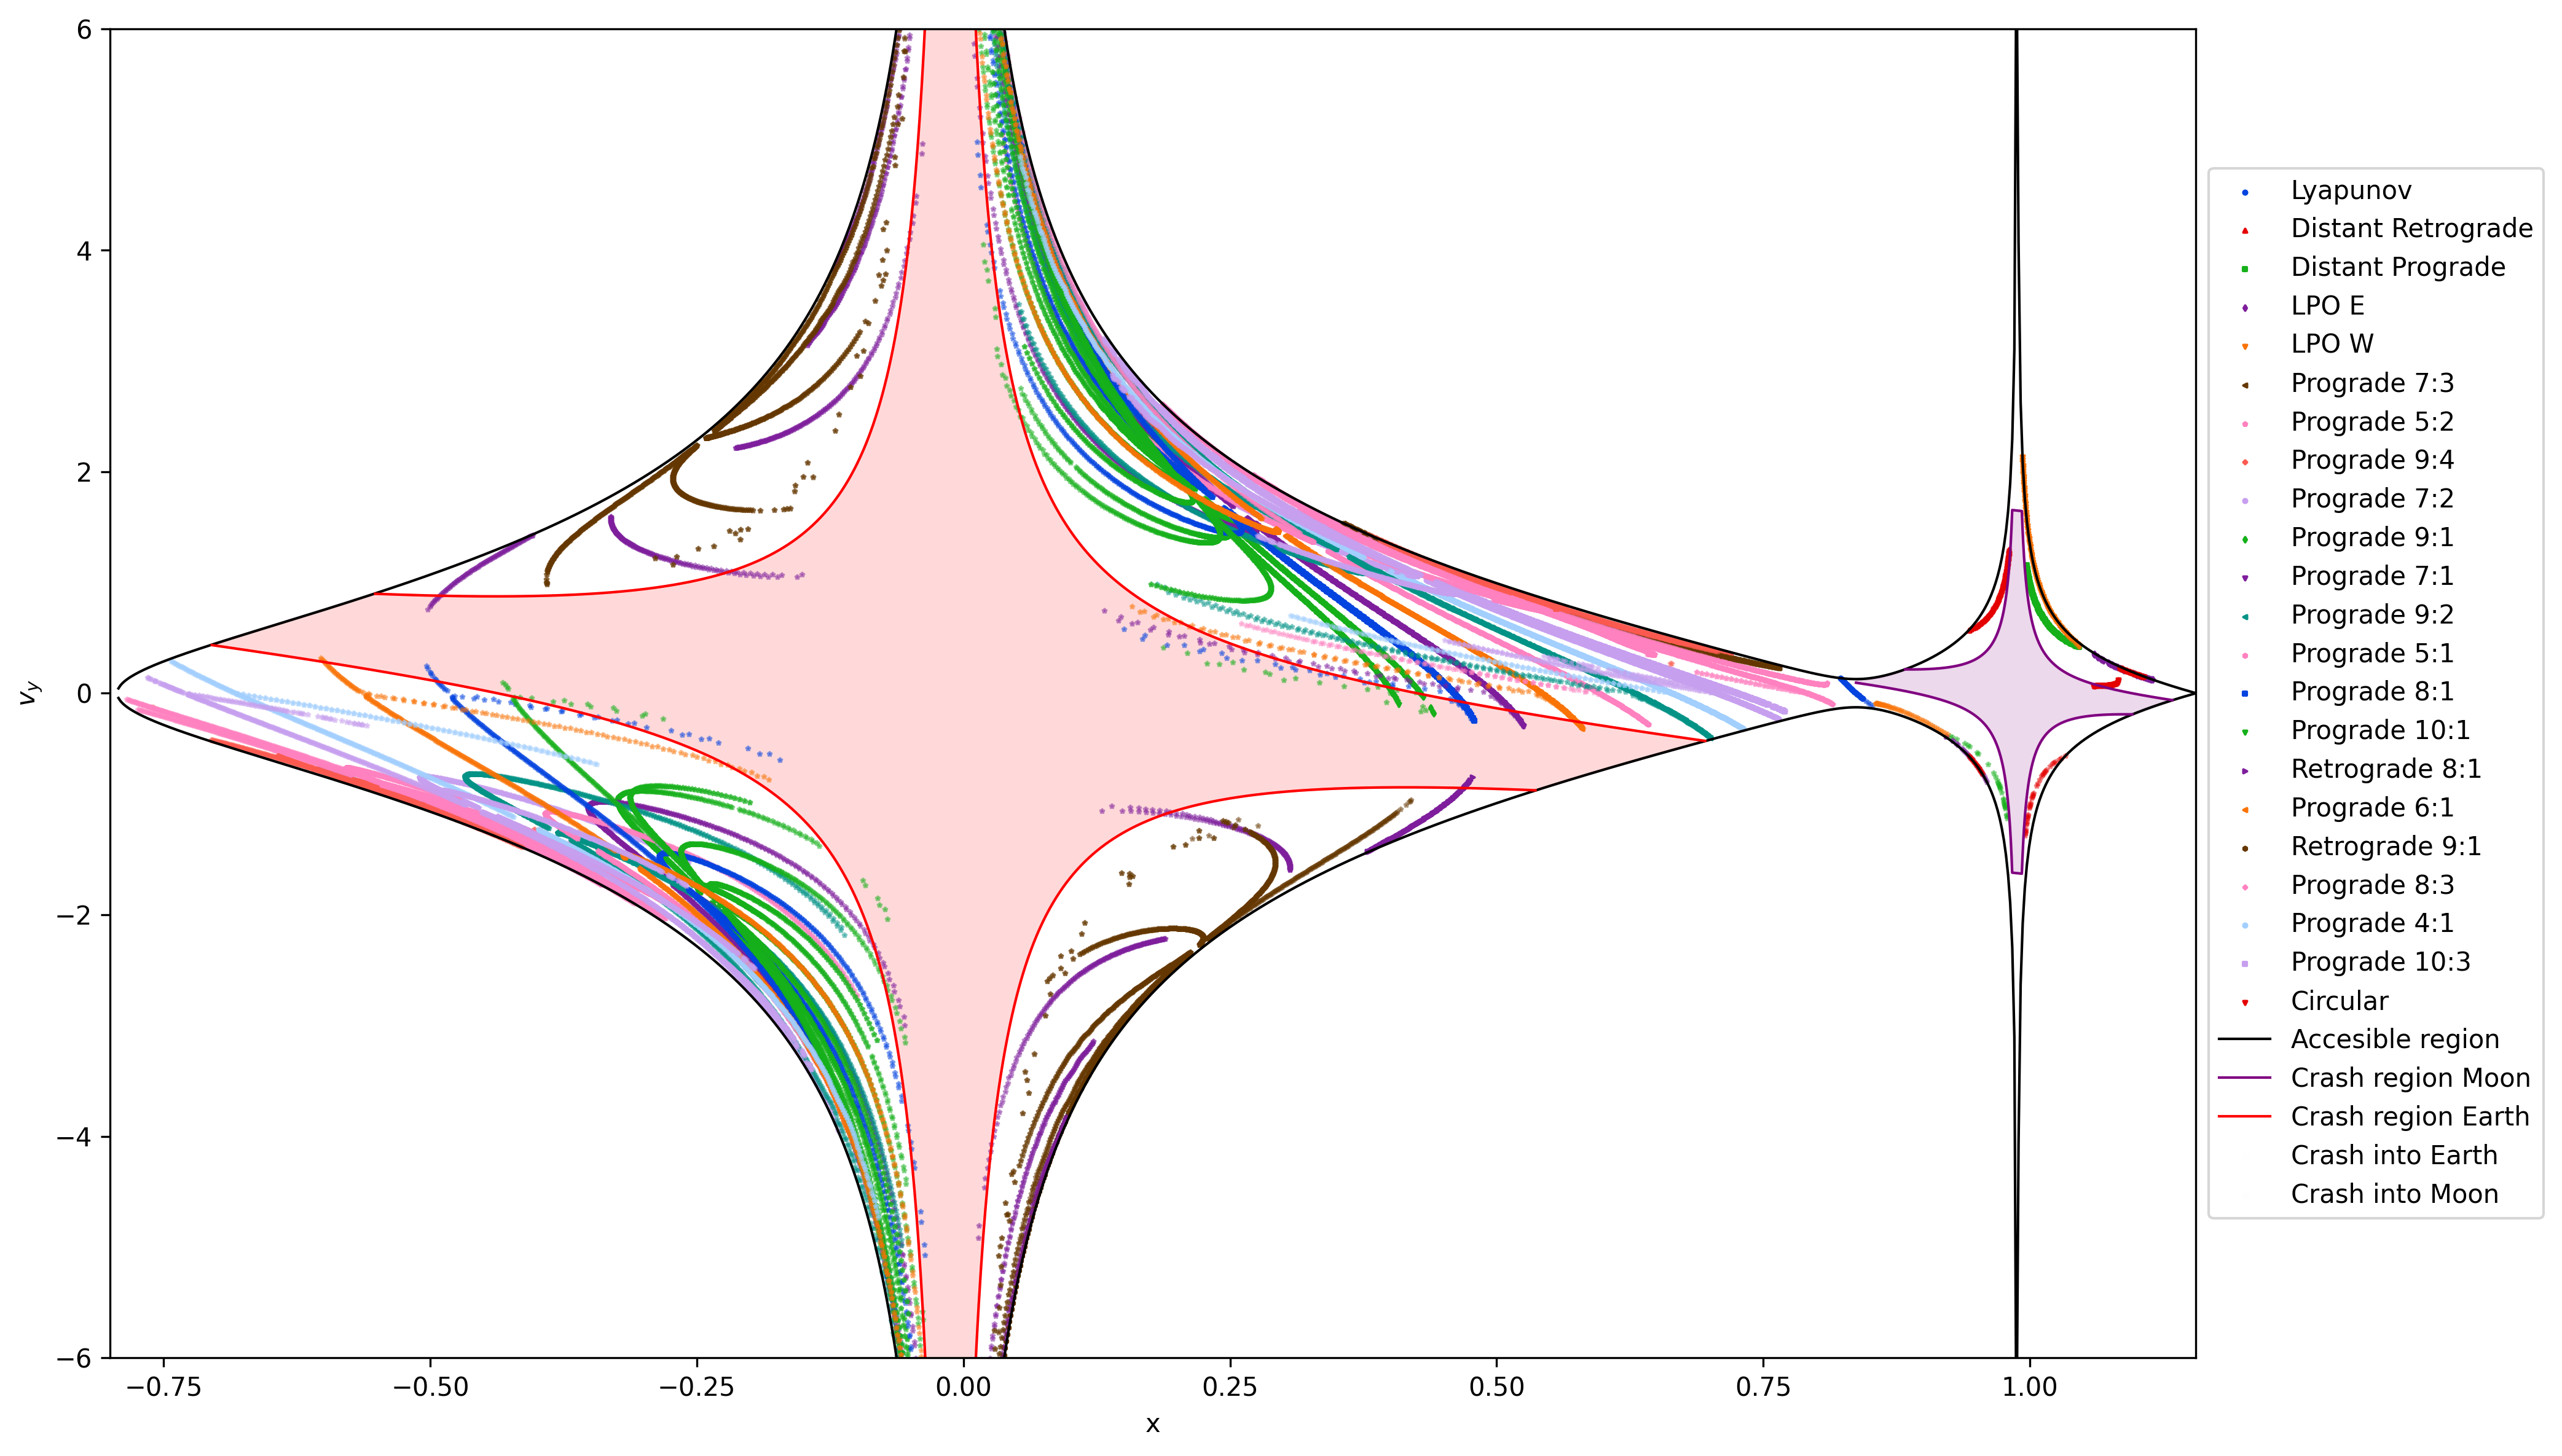
\includegraphics[width=0.75\linewidth]{images/2D crossings all orbits.png}
    %     % \caption{Visualisations of the accessible region in three dimensions and its projection to the $(x,v_y)$ plane, displaying the Earth and Moon crash regions. The larger `pseudosphere'-esque region corresponds to the region around Earth, and the smaller: that of the Moon.}
    %     \caption{Orbital crossings of several planar resonant orbits, depicted in three-dimensions and the projection to the $(x,v_y)$ plane.}
    %     \label{fig: crossings}
    % \end{figure}



    Ultimately, an interesting direction for future work may be investigating the `coverage' of these crossings within our accessible region, potentially finding a method to cover the space with such points to an arbitrary degree.


    Such an effort is not unfounded, results by Poincaré in \cite{Poincare_1893} following a conjecture in \cite{Poincare_1892}, demonstrate the density of periodic orbits at least in analogous, low-energy regimes. It has not been ruled out, and is viewed as likely by the authors and by a larger portion of the astrodynamics community, that this density of periodic orbits may extend to our domain as well.

    Regardless, as can be seen in \cref{fig: crossings}, at least with the families of orbits tested, we have struggled to find families with many crossings close to the inner portion or the space/near the crash region. (Qualitatively, one can see that the points plotted are much more `dense' near the boundary of the accessible region. This is at least true when viewing the upper right and lower left quadrants, as these house the crossings of prograde orbits, which are much more numerous in our tested families due to data availability/the data we computed. Not much should be read into the sparsity of points in the upper left and lower right quadrants (and lunar region), for this reason.)






    \subsection{Chaos in the Cross-Sections}


    In the following \cref{fig: constant energy Poincaré sections}, we briefly provide depictions of the chaos apparent in our system by viewing the action of the Poincaré map on various initial points each with varying colour based on initial location.    
    
    These depictions are done on several Poincaré sections, using the Jacobi constant, $C$, as a proxy for energy. One can see that for $C$ closer to $3.2$, approximately the Jacobi constant correlating to $E_2$ (recall \cref{eq: energy E2}, and that $C = -2E$), the chaotic nature of the system becomes increasingly prominent.
    

    \begin{figure}[h]
        \centering
        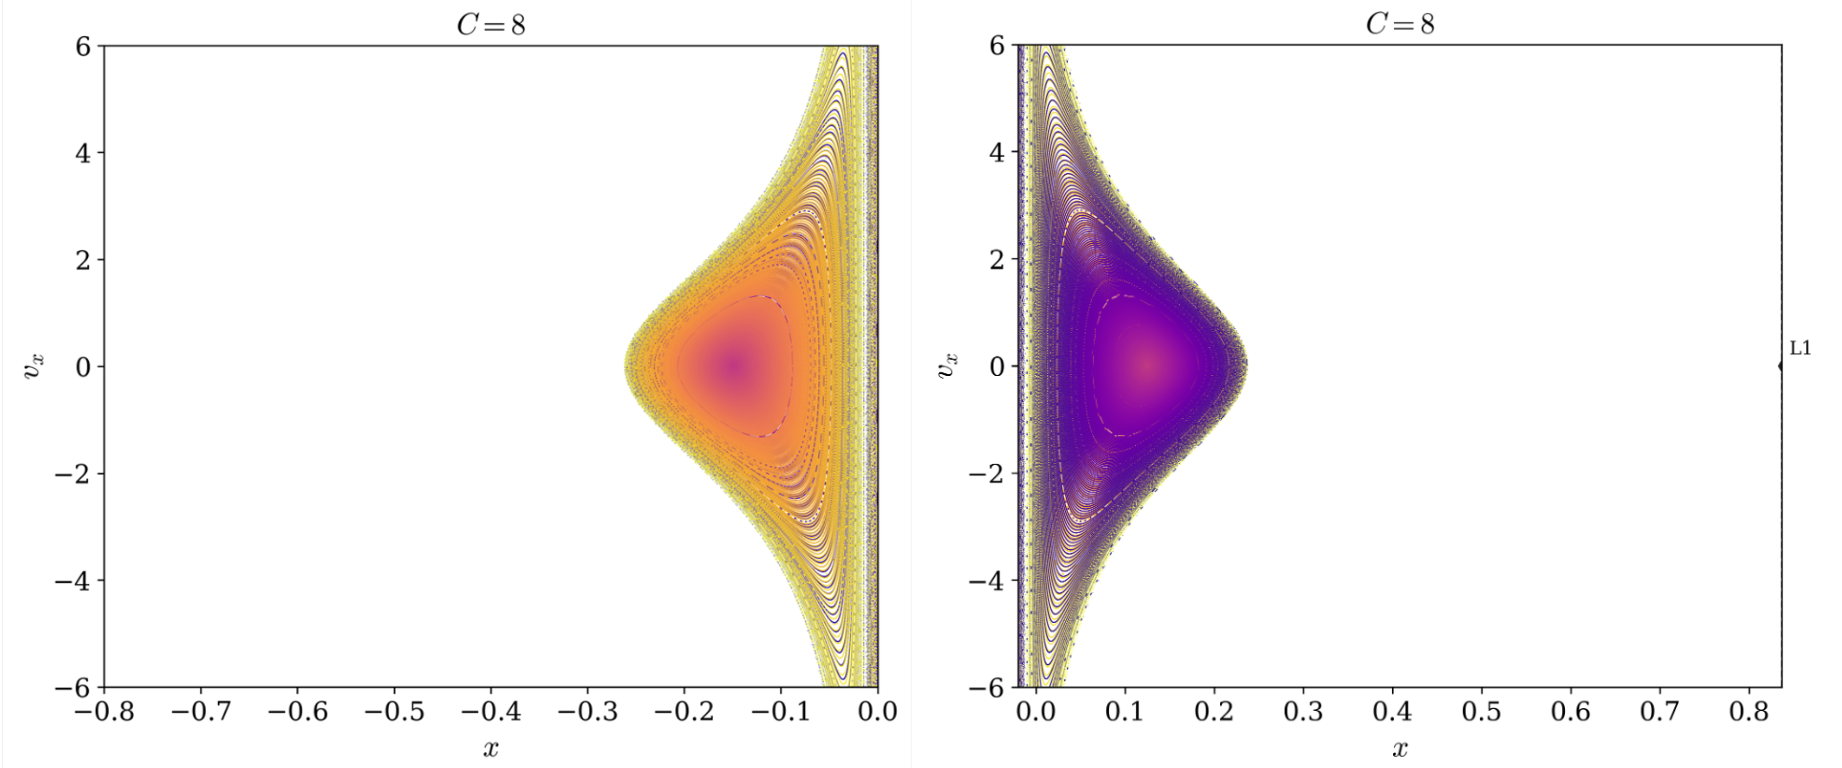
\includegraphics[width=1\linewidth]{images/chaos C 8 .png}
        % 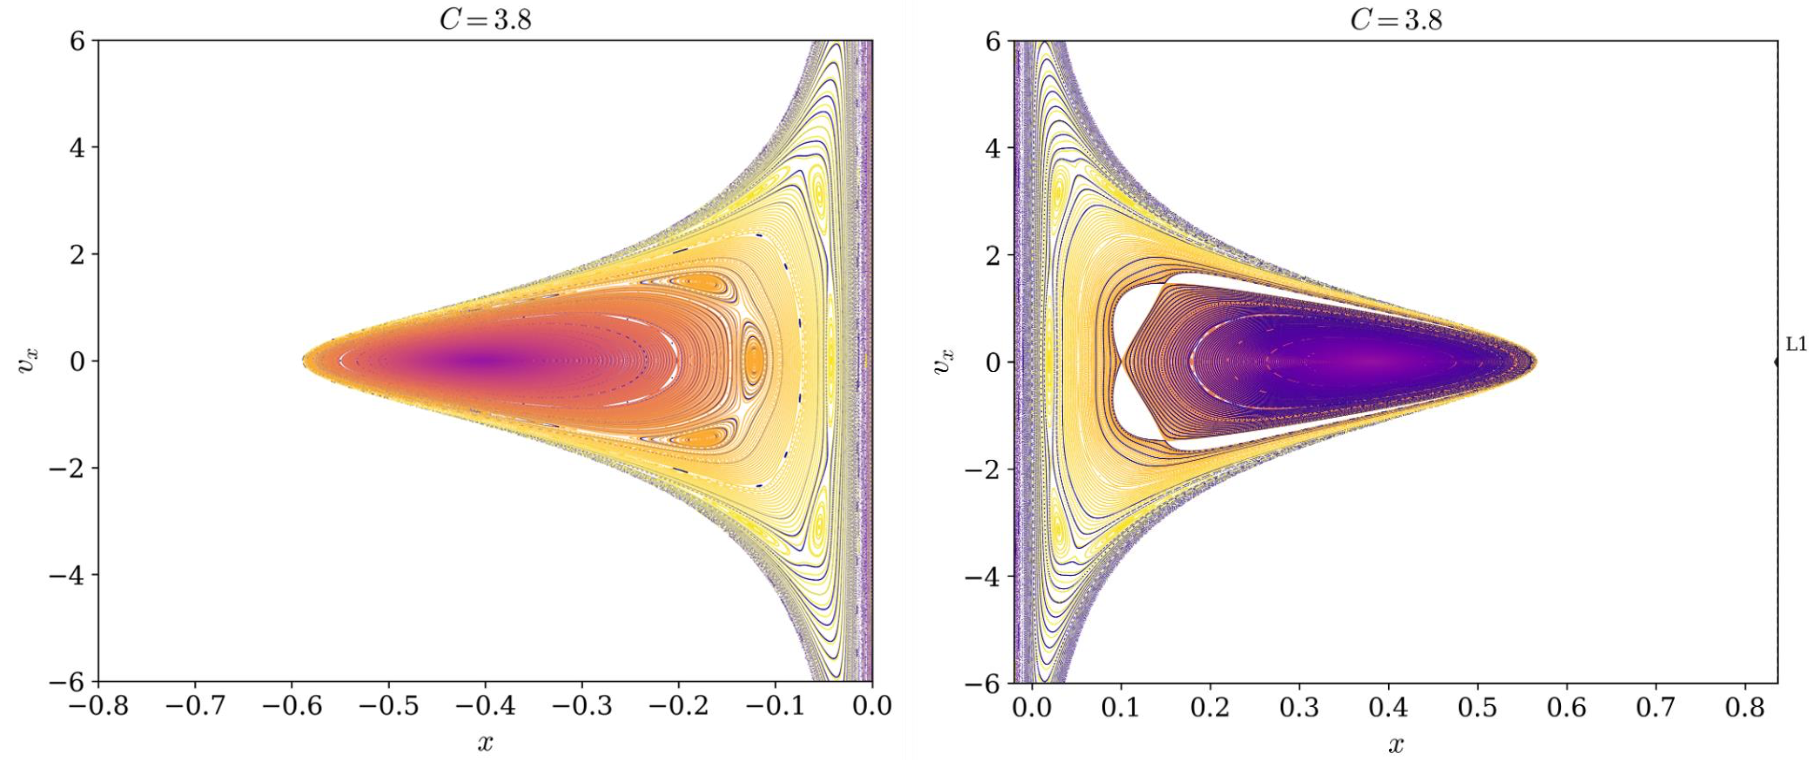
\includegraphics[width=1\linewidth]{images/chaos C 3.8 .png}
        % 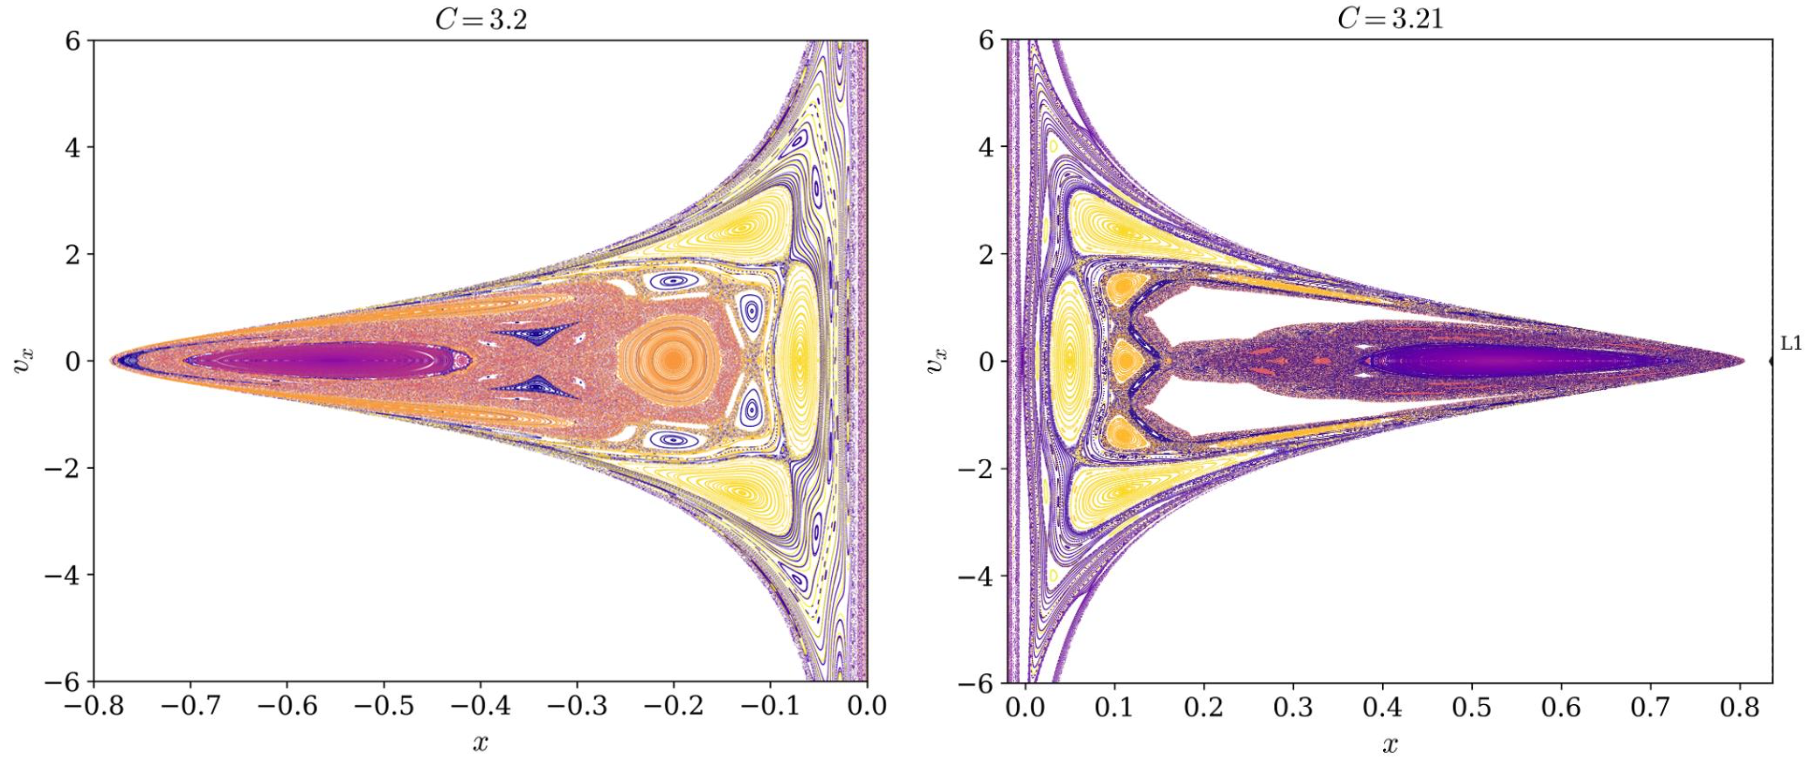
\includegraphics[width=1\linewidth]{images/chaos C 3.2 .png}
        \caption{Poincaré sections for different Jacobi constants.}
        \label{fig: constant energy Poincaré sections}
    \end{figure}

    
    \begin{figure}[h]
        \centering
        % 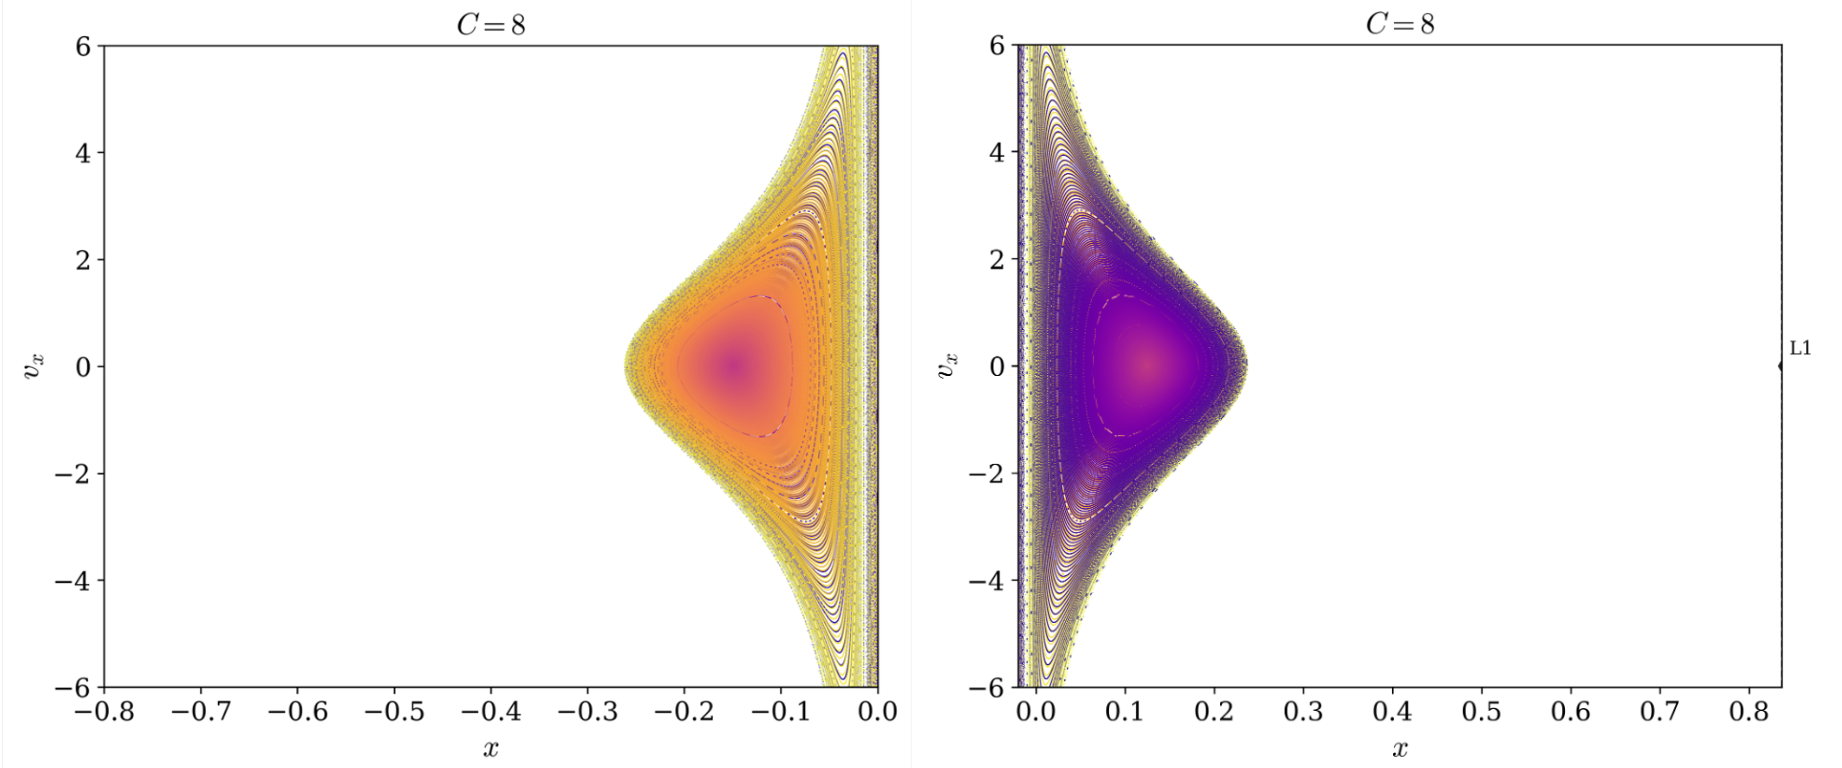
\includegraphics[width=1\linewidth]{images/chaos C 8 .png}
        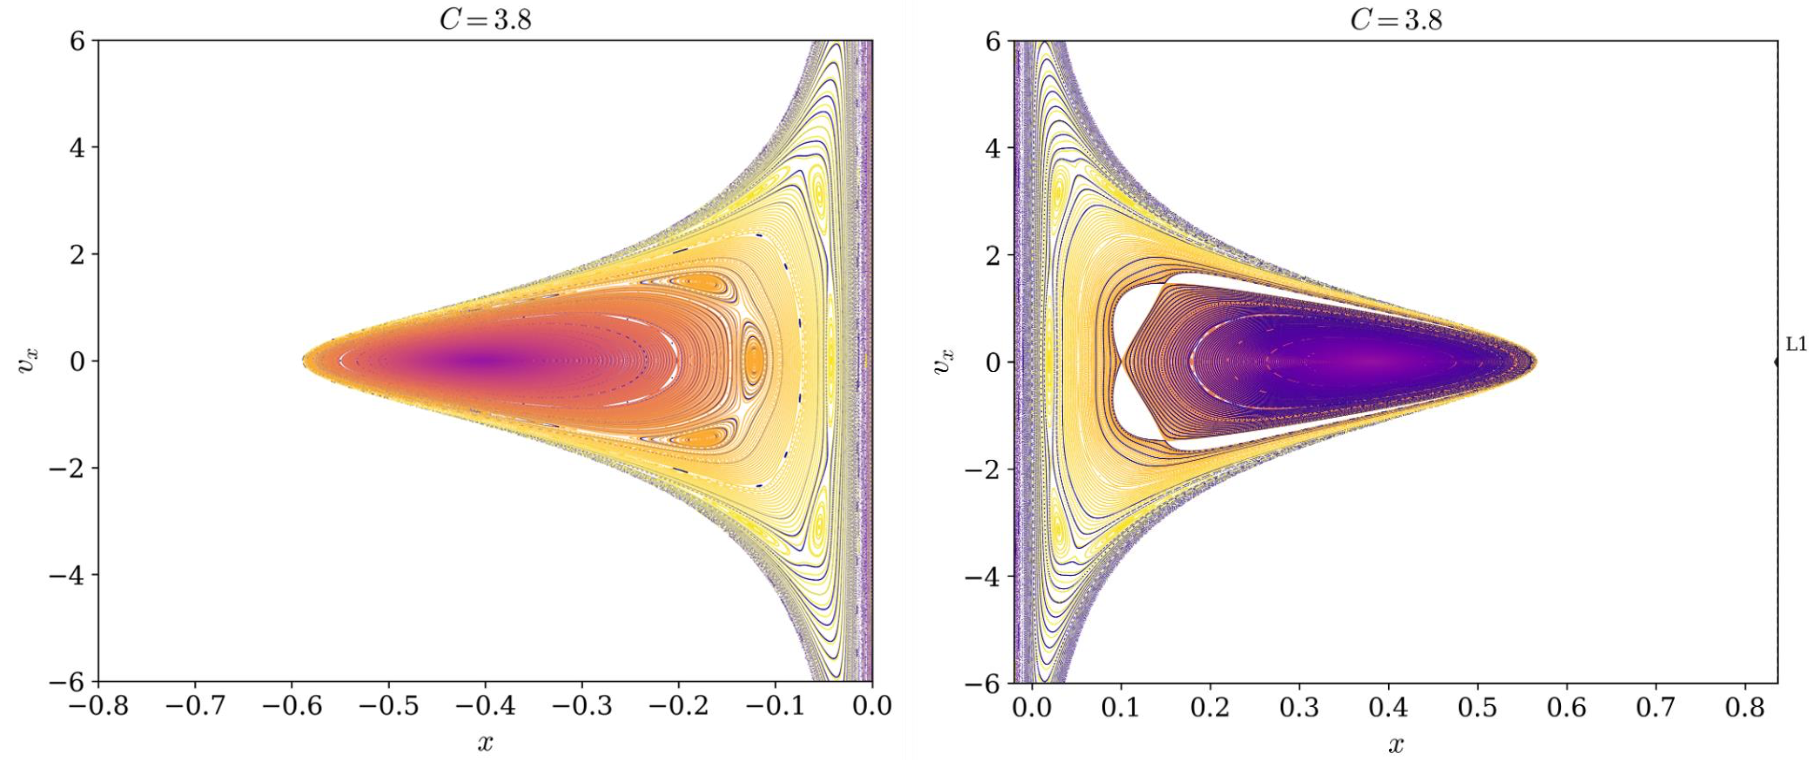
\includegraphics[width=0.81\linewidth]{images/chaos C 3.8 .png}
        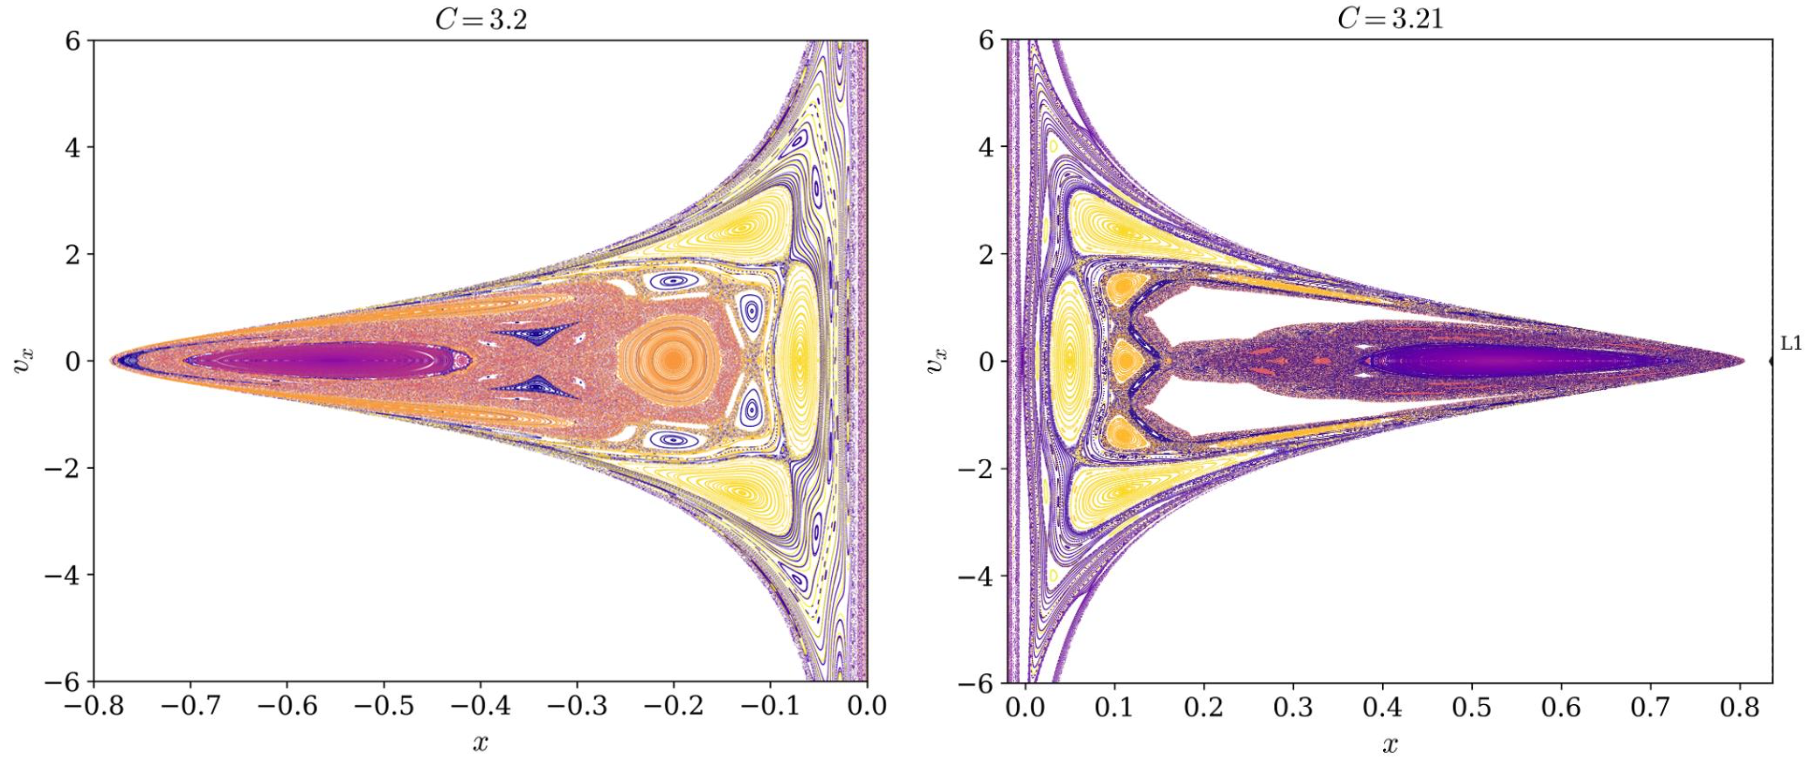
\includegraphics[width=0.81\linewidth]{images/chaos C 3.2 .png}
        % \label{fig: constant energy Poincaré sections}
    \end{figure}



    % \begin{figure}[h]
    %     \centering
    %     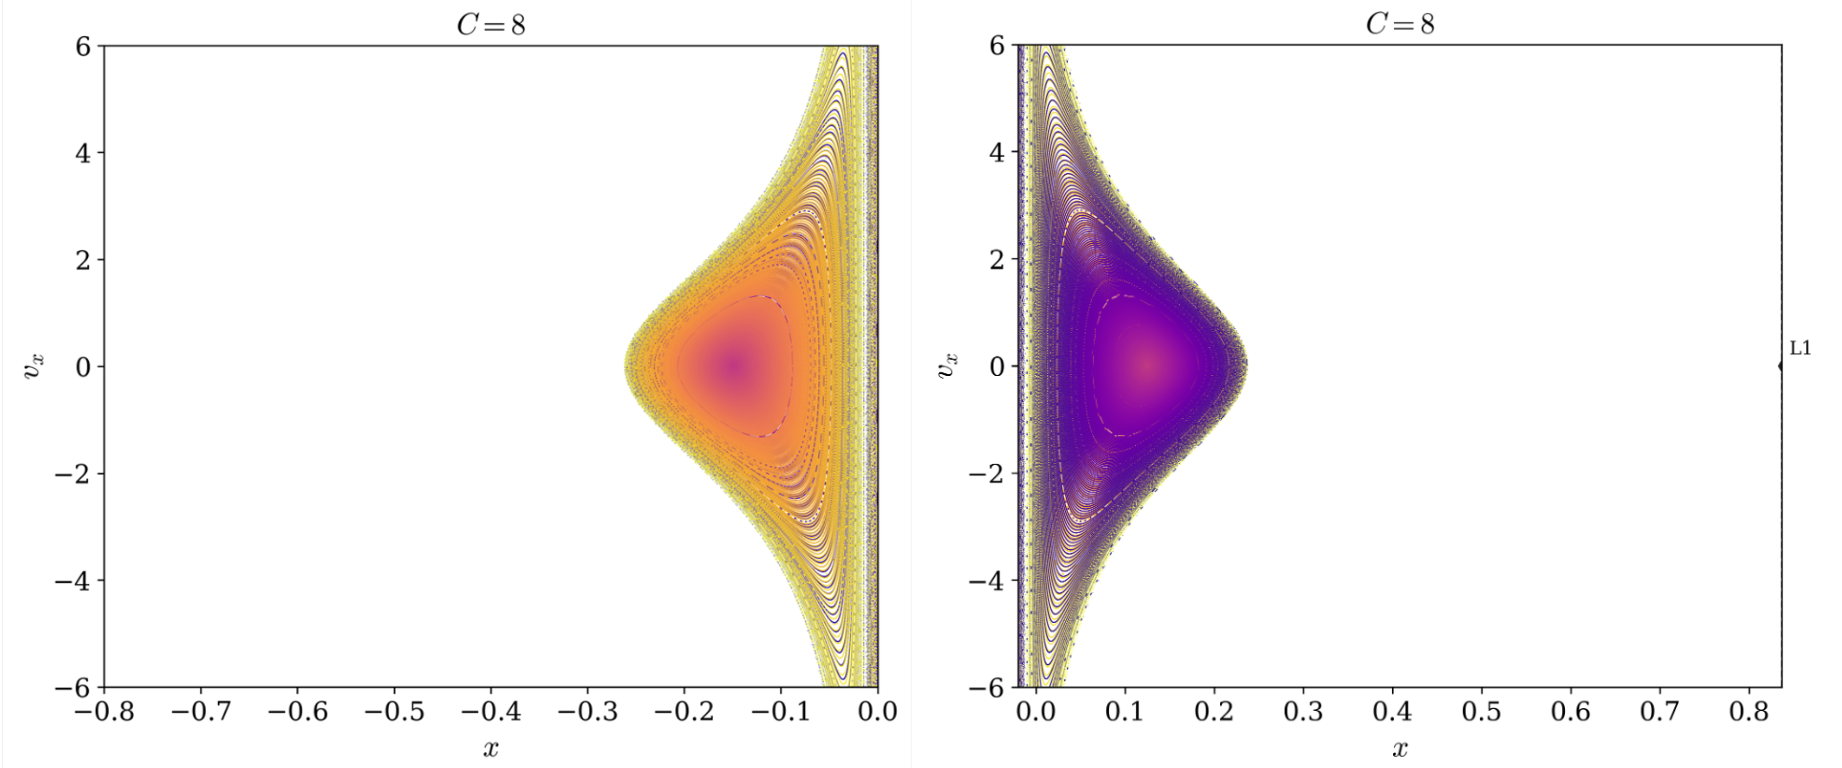
\includegraphics[width=0.8\linewidth]{images/chaos C 8 .png}
    %     % \caption{Poincaré sections for constant Jacobi constants.}
    %     % \label{fig: constant energy Poincaré sections}
    % \end{figure}
    
    % \begin{figure}[h]
    %     \centering
    %     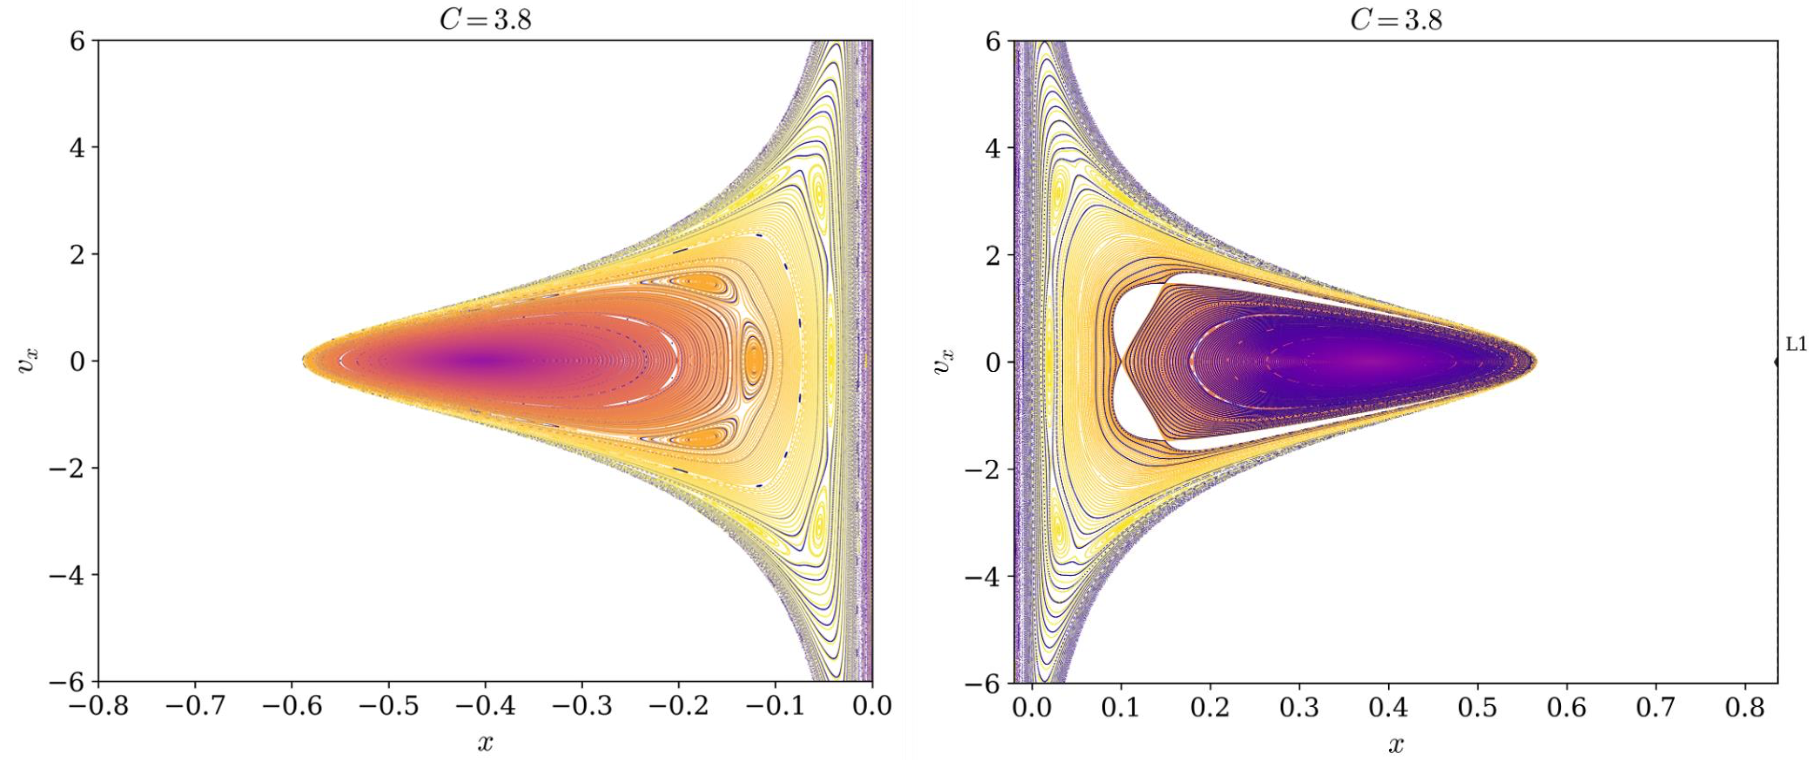
\includegraphics[width=0.8\linewidth]{images/chaos C 3.8 .png}
    %     % \caption{Poincaré sections for constant Jacobi constants.}
    %     % \label{fig: constant energy Poincaré sections}
    % \end{figure}

    % \begin{figure}[h]
    %     \centering
    %     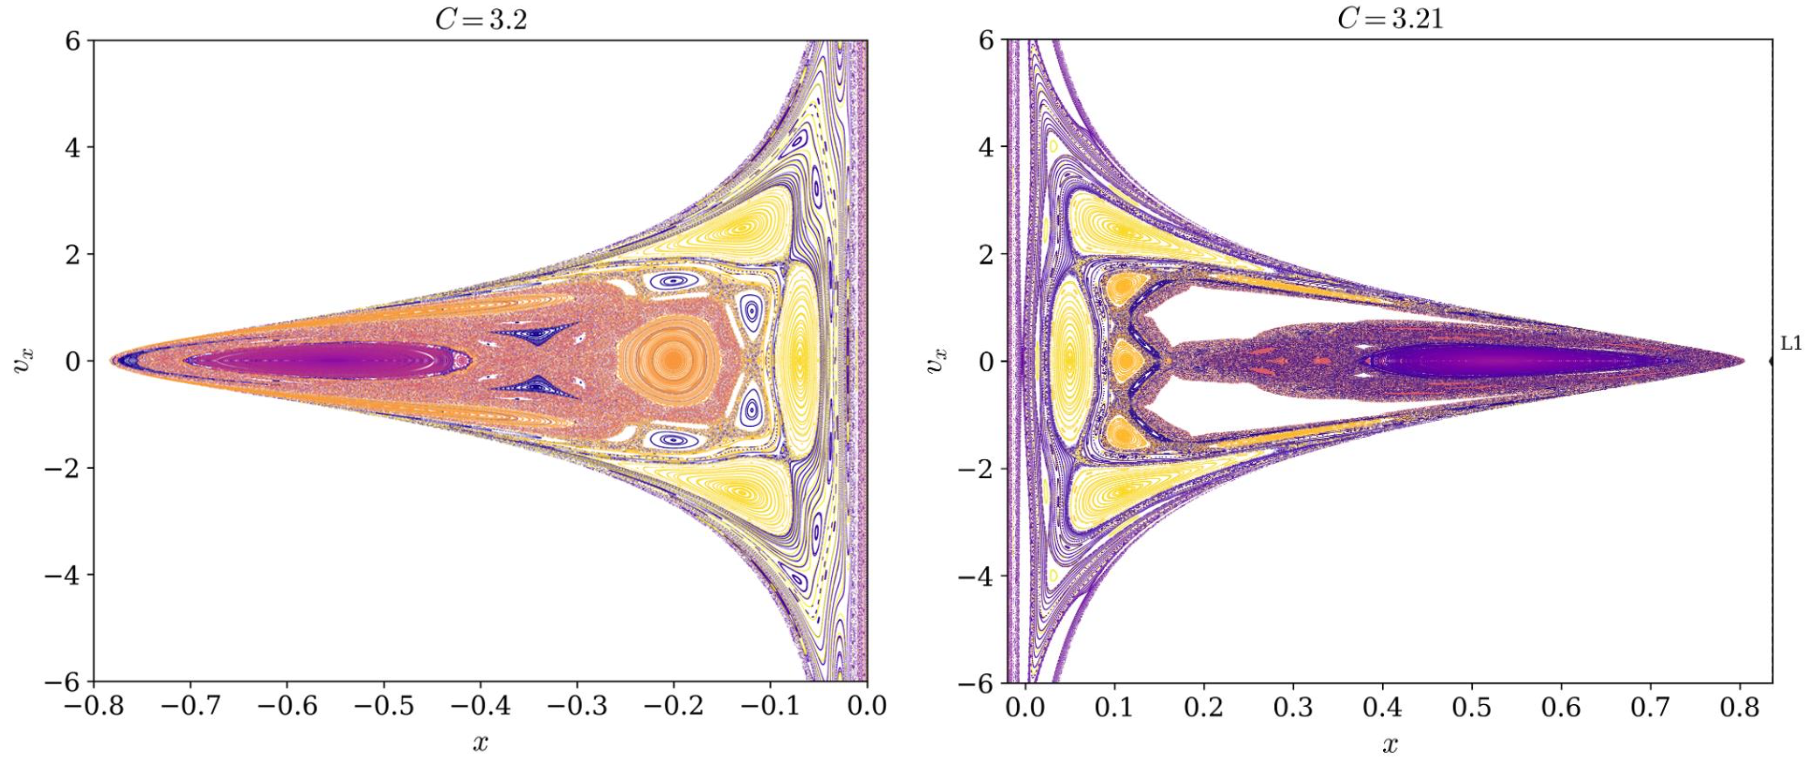
\includegraphics[width=0.8\linewidth]{images/chaos C 3.2 .png}
    %     % \caption{Poincaré sections for constant Jacobi constants.}
    %     % \label{fig: constant energy Poincaré sections}
    % \end{figure}





    Further, the large `islands of stability', prominent in \cref{fig: constant energy Poincaré sections} and characterised by concentric rings, are nicely centred around low ratio $p:q$ resonant orbits. \cref{fig: Jannik's nice poincare pq diagram} provides a particularly enlightening depiction of several of these points.

    \vspace{1cm}

    \begin{figure}[hbt]
        \centering
        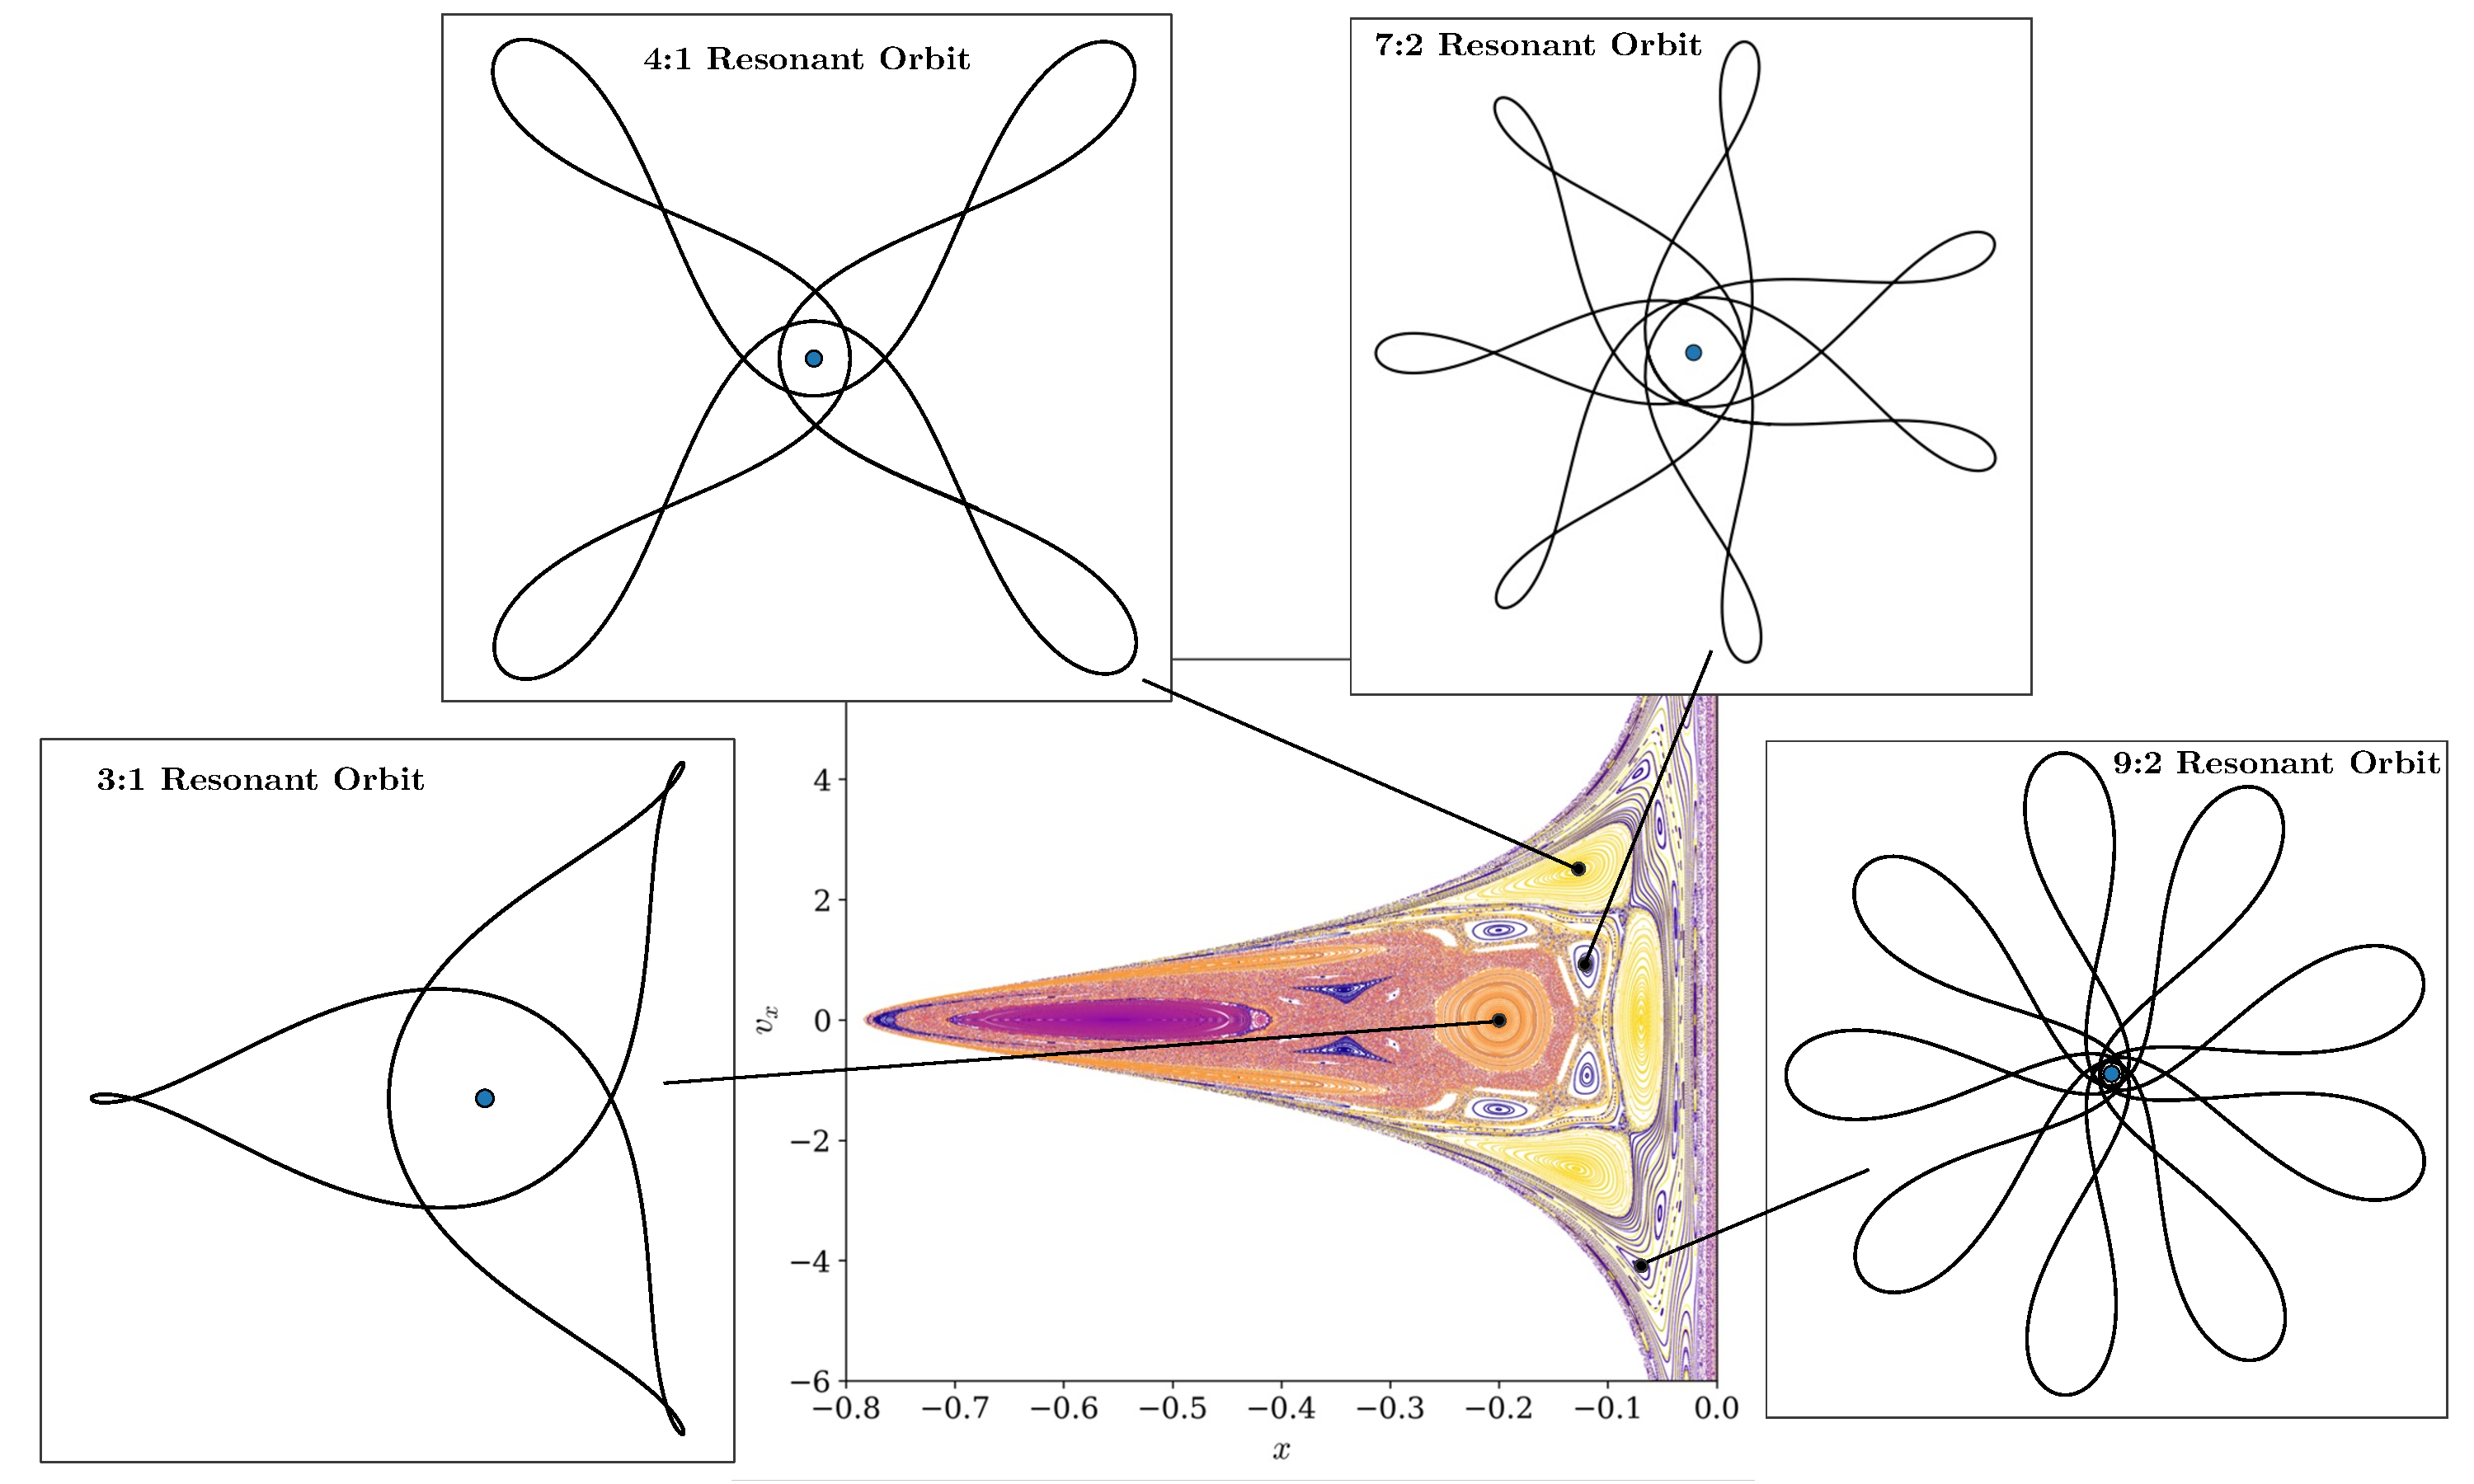
\includegraphics[width=0.7\linewidth]{images/Chaotic_sea_figure.pdf}
        \caption{Depiction of several stable points in the $C=3.2$ diagram corresponding to low ratio $p:q$ resonant orbits.}
        \label{fig: Jannik's nice poincare pq diagram}
    \end{figure}

\newpage %temporarily


\section{Bifurcations of Periodic Orbits} \label{sec:Bifurcations}

\newpage %temporarily

\newpage
\section{Normal Forms Around Periodic Orbits} \label{sec:NormalForms}

Normal form theory provides a systematic way to simplify a non-linear dynamical system near an invariant object through a suitable change of coordinates. 
The central idea is to apply a sequence of near-identity transformations that remove non-essential non-linear terms while retaining the dominant structure of the dynamics. 
For Hamiltonian systems, such as the CR3BP, these transformations must be symplectic so that the Hamiltonian structure of the original system is preserved. 
The resulting simplified system is advantageous because its dynamics can be described analytically, enabling closed-form propagation in the transformed coordinates. 
As a result, the long-term evolution of objects near a periodic orbit can be approximated in a single evaluation rather than through computationally expensive numerical integration over many years or decades. 
This capability is particularly useful for applications such as predicting the evolution of space debris in the cislunar domain over long time-horizons. 
In the following, we provide an overview of normal form theory in the context of periodic orbits in the CR3BP and present numerical results demonstrating its application.

\subsection{Normal Form Theory}
This section provides only a concise overview of the normal form transformations used in this work; a more complete theoretical description can be found in Sinha's dissertation \cite{Sinha2026}. 
The methodology follows the numerical normal form framework developed by Jorba and Villanueva \cite{Jorba1998,Jorba1999}. 
The implementation used in the present analysis was developed with contributions from Sinha \cite{Sinha2026} and is applied here to the examples considered below. 
We describe the transformations at a high level and emphasize how the Hamiltonian changes at each step.
For a Hamiltonian $H$, the equations of motion in canonical coordinates can be written as
\begin{equation}
    \dot{\boldsymbol{x}} = \boldsymbol{J} \nabla H(\boldsymbol{x}), \qquad
    \boldsymbol{J} = \begin{pmatrix}
    0 & I \\
    - I & 0
    \end{pmatrix},
\end{equation}
where $\boldsymbol{J}$ is the canonical symplectic matrix. 
The coordinate transformations used below are symplectic, meaning that they preserve this canonical Hamiltonian structure.

Let the periodic orbit be denoted by $\boldsymbol{\gamma}:\mathbb{R}\rightarrow\mathbb{R}^6$, with $\boldsymbol{\gamma}(t+T)=\boldsymbol{\gamma}(t)$. 
The first step in constructing the normal form is to translate the periodic orbit to the origin using
\begin{equation}
    \boldsymbol{\xi}=\boldsymbol{x}-\boldsymbol{\gamma}(t).
\end{equation}
The Hamiltonian in the translated coordinates, denoted by $K_1(t,\boldsymbol{\xi})$, is time dependent. 
Expanding about $\boldsymbol{\xi}=0$ gives
\begin{equation}
K_1(t,\boldsymbol{\xi})
=
\frac{1}{2}\boldsymbol{\xi}^{T}
\nabla^2 H(\boldsymbol{\gamma}(t))
\boldsymbol{\xi}
+
\sum_{d \geq 3} H_d^{(\boldsymbol{\xi})}(t,\boldsymbol{\xi}),
\end{equation}
where $\nabla^2 H(\boldsymbol{\gamma}(t))$ is the Hessian of the original Hamiltonian evaluated along the periodic orbit, and $H_d^{(\boldsymbol{\xi})}$ denotes the homogeneous polynomial terms of degree $d$ in $\boldsymbol{\xi}$. 
The constant and linear terms vanish because the expansion is taken about the translated periodic solution.

The next transformation removes the explicit time dependence from the quadratic part of the Hamiltonian. 
This is achieved through a Floquet transformation to new coordinates $\boldsymbol{\eta}$,
\begin{equation}
    \boldsymbol{\eta}=\boldsymbol{P}^{-1}(t)\boldsymbol{\xi}.
\end{equation}
Here, $\boldsymbol{P}(t)$ is the periodic part of the STM decomposition
\begin{equation}
\label{eq: STM decomposition}
\boldsymbol{\Phi}(t) = \boldsymbol{P}(t)e^{t\boldsymbol{B}},
\end{equation}
where $\boldsymbol{P}(t+T)=\boldsymbol{P}(t)$ and $\boldsymbol{P}(0)=\boldsymbol{I}$. 
The matrix $\boldsymbol{\Phi}(t)$ is the STM of the variational dynamics in the translated $\boldsymbol{\xi}$ coordinates, defined in the same sense as Eq. \eqref{eq: STM} and $\boldsymbol{B}$ is a Floquet exponent matrix. 
Once $\boldsymbol{B}$ is determined from
\begin{equation}
    \boldsymbol{B} = \frac{1}{T}\log\!\left(\boldsymbol{\Phi}(T)\right),
\end{equation}
the periodic matrix $\boldsymbol{P}(t)$ follows from \cref{eq: STM decomposition}. 
In Floquet coordinates, the Hamiltonian takes the form
\begin{equation}
    K_2(t,\boldsymbol{\eta}) 
    = \frac{1}{2}\boldsymbol{\eta}^{\top} \boldsymbol{S} \boldsymbol{\eta} 
    + \sum_{d \ge 3} H_d^{(\boldsymbol{\eta})}(t,\boldsymbol{\eta}),
\end{equation}
where the quadratic part is now autonomous and $\boldsymbol{S}=-\boldsymbol{J}\boldsymbol{B}$.

The remaining transformations remove higher-order nonresonant terms from the Hamiltonian. 
At each degree $d$, this is done by solving the homological equation
\begin{equation}
    \label{eq: homological equation}
    \mathcal{L}_d W_d + Z_d = H_d^{(\boldsymbol{\eta})}.
\end{equation}
Here, $W_d(t,\boldsymbol{\eta})$ is the generating function of the near-identity transformation, and $Z_d$ contains the terms that remain in the normal form. 
Ideally, $W_d$ is chosen so that $Z_d=0$; however, terms that lie in the kernel of the homological operator cannot be removed and are retained as resonant terms. 
The homological operator is defined as
\begin{equation}
    \mathcal{L}_d W 
    \equiv \partial_t W + \{ W, H_2 \}, 
    \qquad 
    \{ W, H_2 \} \equiv \nabla W^{\top} J \nabla H_2,
\end{equation}
where $H_2=\frac{1}{2}\boldsymbol{\eta}^{\top}\boldsymbol{S}\boldsymbol{\eta}$ is the quadratic Hamiltonian.

Since the higher-order terms remain time periodic, they can be expanded in a Fourier series,
\begin{equation}
    H_d^{(\boldsymbol{\eta})}(t,\boldsymbol{\eta})
    =
    \sum_{|k|\le K} H_{d,k}(\boldsymbol{\eta}) e^{ik\omega t},
    \qquad 
    \omega = \frac{2\pi}{T},
\end{equation}
where the series is truncated at Fourier order $K$. 
Expanding $W_d$ and $Z_d$ in the same form decouples the homological equation by polynomial degree and Fourier mode, allowing the normal form transformation to be computed term by term.

The final Hamiltonian consists of the autonomous quadratic part together with the resonant higher-order terms that cannot be removed. 
It defines the approximate dynamics in the normal form coordinates $\boldsymbol{u}$, in which objects can be propagated analytically.

\subsection{Numerical Results}

We test the normal form construction using a planar Lyapunov orbit around the libration point $\mathcal{L}_1$. 
The orbit is shown in \cref{fig:ex_lyap} together with its Floquet multipliers, defined as the eigenvalues of the monodromy matrix. 
Because the orbit lies in a region where the gravitational influence of both the Earth and the Moon is significant, its dynamics are highly unstable, as indicated by the multiplier far outside the unit circle. 
This instability makes the orbit a challenging test case for the normal form approximation.

\begin{figure}[t!]
    \centering
    \begin{subfigure}{0.29\textwidth}
        \centering
        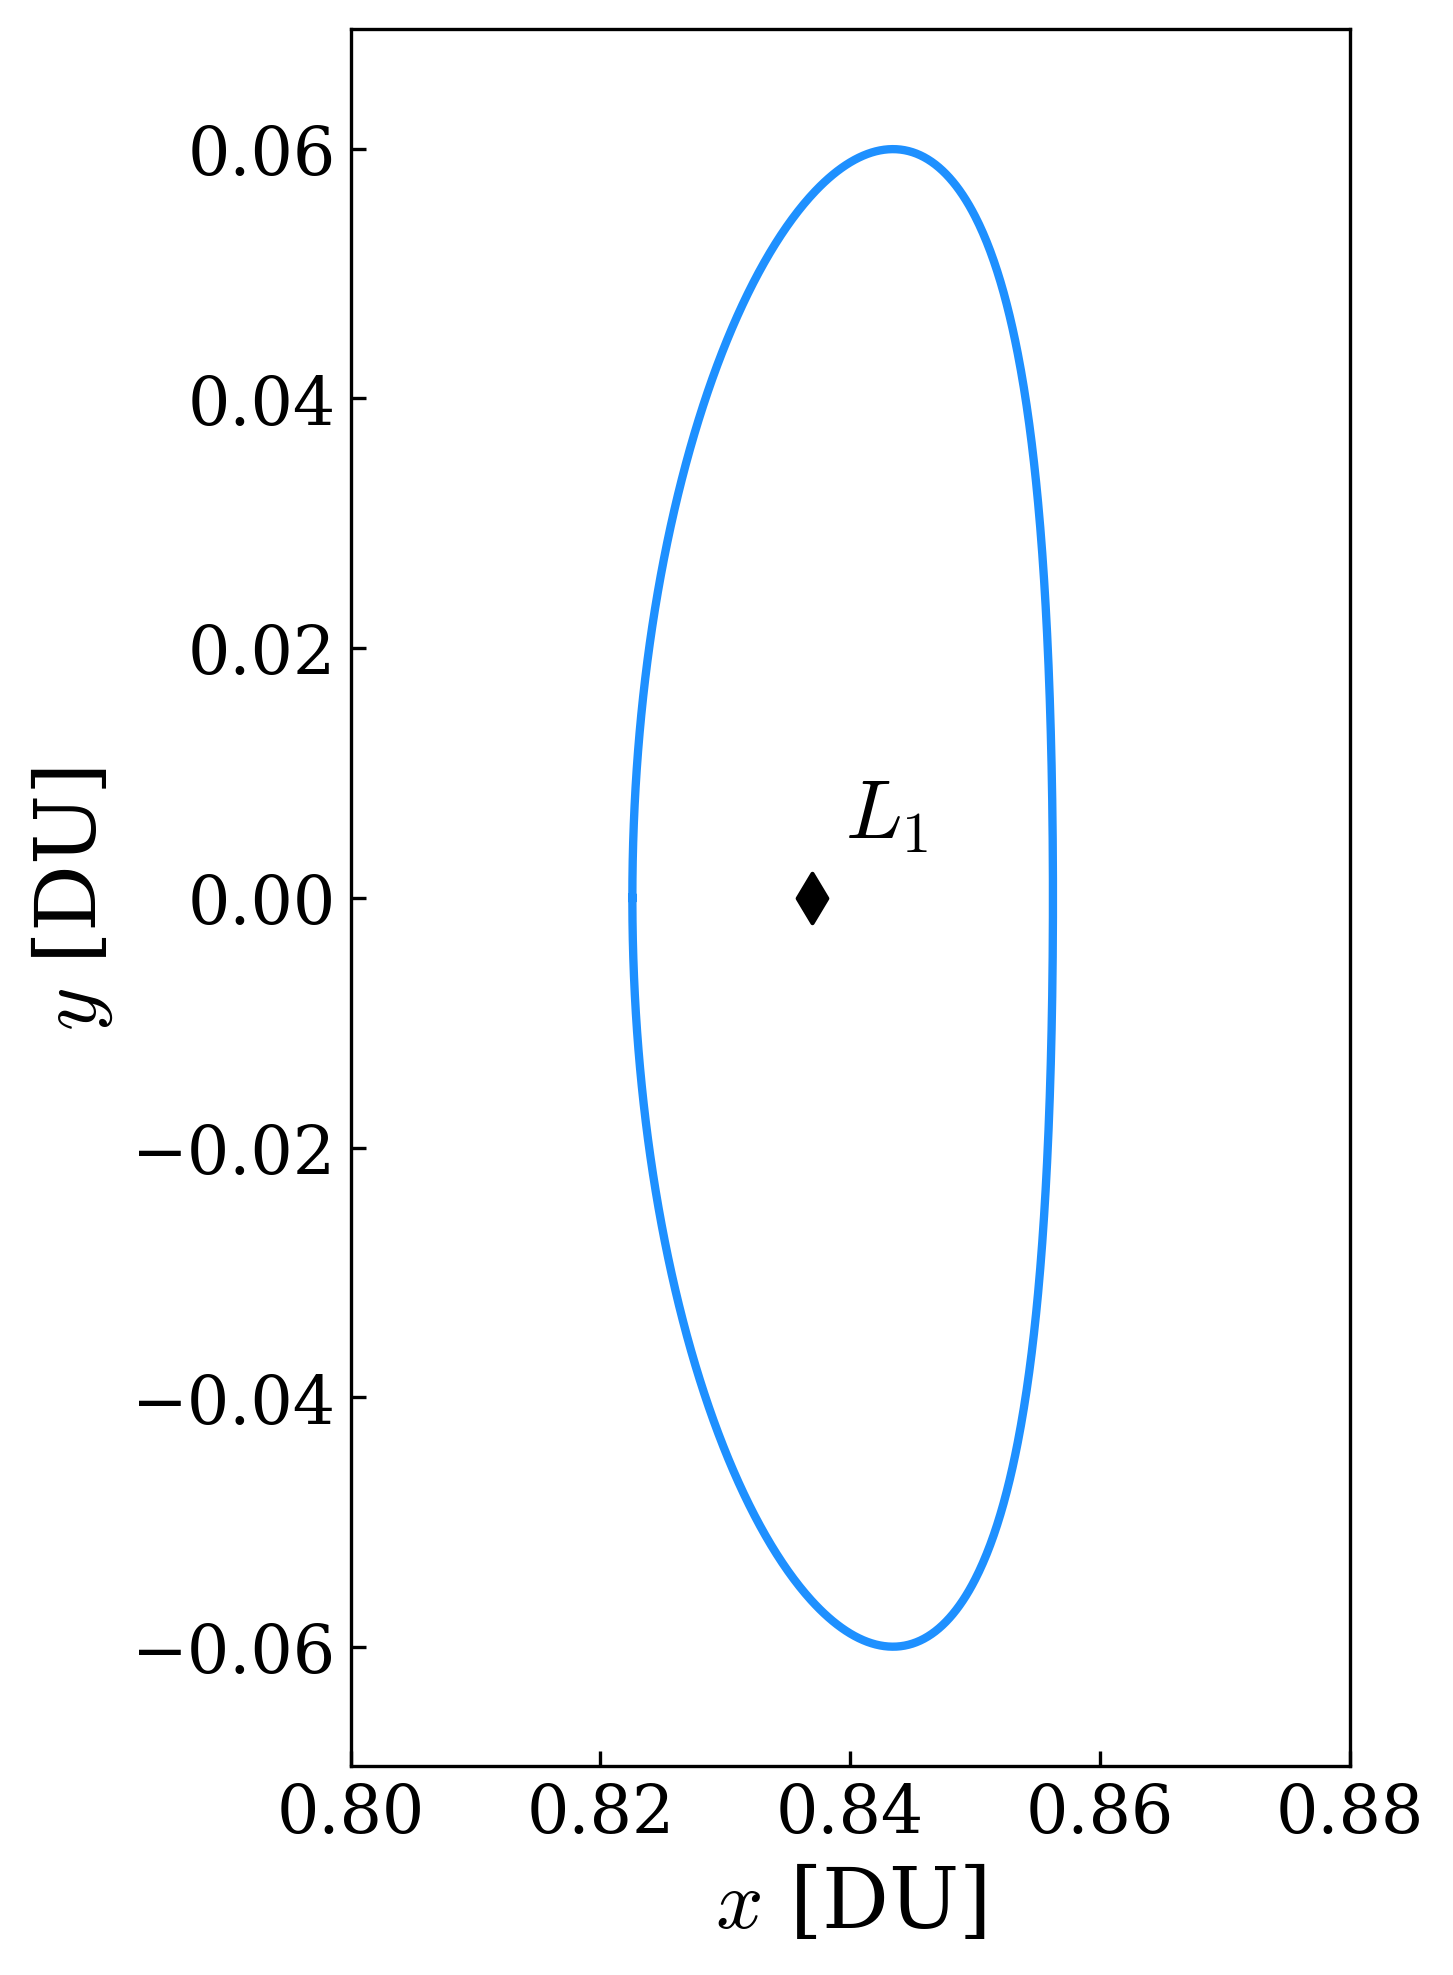
\includegraphics[height=6.3cm,keepaspectratio]{images/lyapunov_orbit_xy.png}
        \caption{Trajectory in $x$-$y$.}
        \label{fig:traj}
    \end{subfigure}
    \hfill
    \begin{subfigure}{0.69\textwidth}
        \centering
        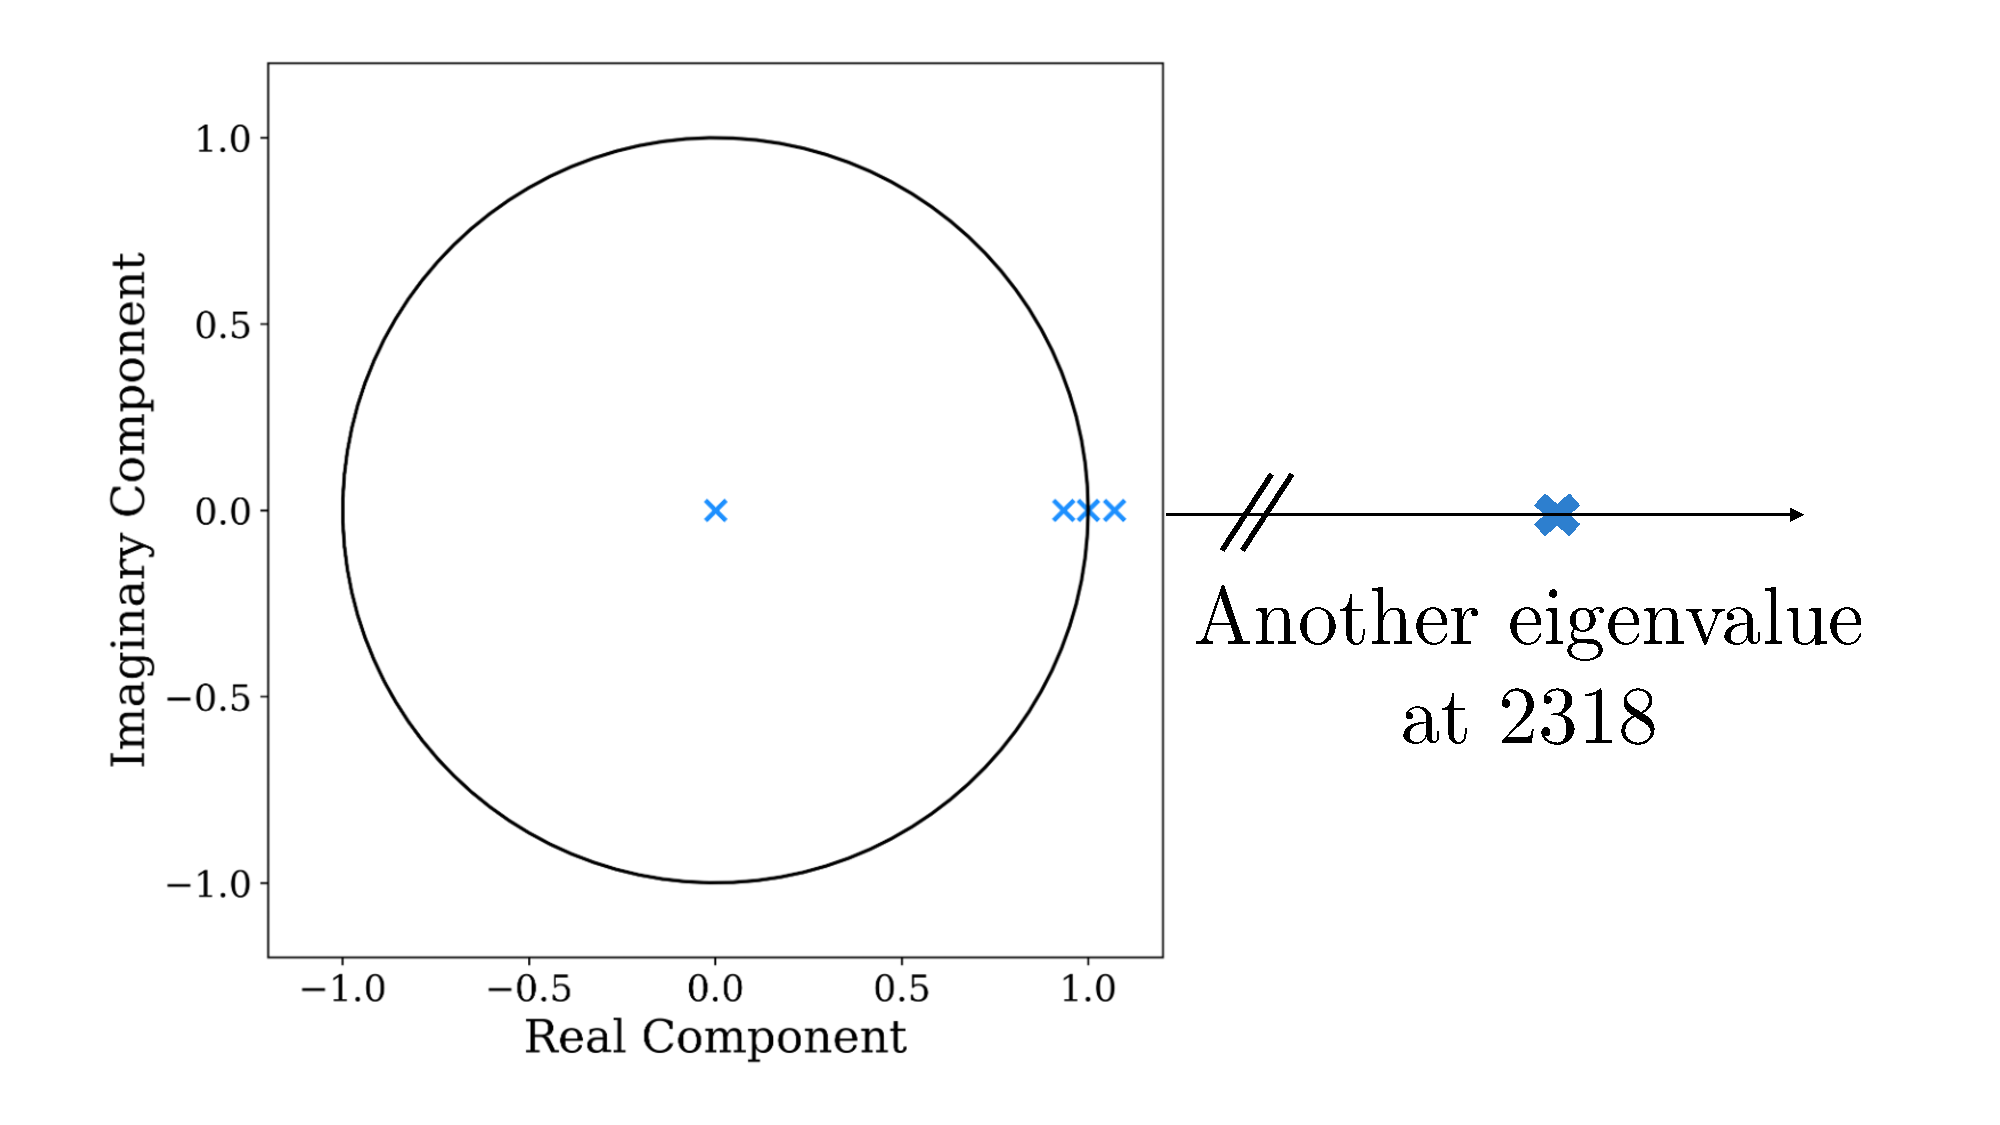
\includegraphics[height=6.3cm,keepaspectratio]{images/floquet_plot.pdf}
        \caption{Floquet multipliers in the complex plane.}
        \label{fig:floq}
    \end{subfigure}

    \caption{Planar Lyapunov orbit used to test the normal form construction.}
    \label{fig:ex_lyap}
\end{figure}

To demonstrate the application of the normal form, we initialize a set of nearby trajectories from a Gaussian distribution centered on the Lyapunov orbit and propagate them using both the full synodic CR3BP dynamics and the simplified normal form system. 
The initial Gaussian is sampled on the Poincaré section $y=0$ around the initial crossing point of the Lyapunov orbit. 
The standard deviations are chosen as 
$\sigma_x = 10^{-6}\,\mathrm{DU}\,(384\,\mathrm{m})$, 
$\sigma_{v_x} = 10^{-4}\,\mathrm{VU}\,(0.1\,\mathrm{m}/\mathrm{s})$, and
$\sigma_{v_y} = 10^{-4}\,\mathrm{VU}\,(0.1\,\mathrm{m}/\mathrm{s})$.
We draw $100$ samples from this distribution and map each sample to normal form coordinates using the transformations $\boldsymbol{x}\rightarrow\boldsymbol{u}$ described above. 
To limit the computational cost, the normal form is truncated at polynomial degree $D=4$, and the time-periodic coefficients are represented using a Fourier expansion of order $K=16$. 
The samples are then propagated analytically in normal form coordinates for one orbital period. 
For comparison, the same initial conditions are propagated in the synodic CR3BP coordinates using an adaptive step-size RK54 integrator. 
To compare both propagation methods, the analytically propagated normal form trajectories are mapped back to the synodic frame through the inverse transformation $\boldsymbol{u}\rightarrow\boldsymbol{x}$ at the same time instances used by the numerical integrator. 
The results are shown in \cref{fig:nf_comparison}.

\begin{figure}[b!]
    \centering
    \begin{subfigure}{0.39\textwidth}
        \centering
        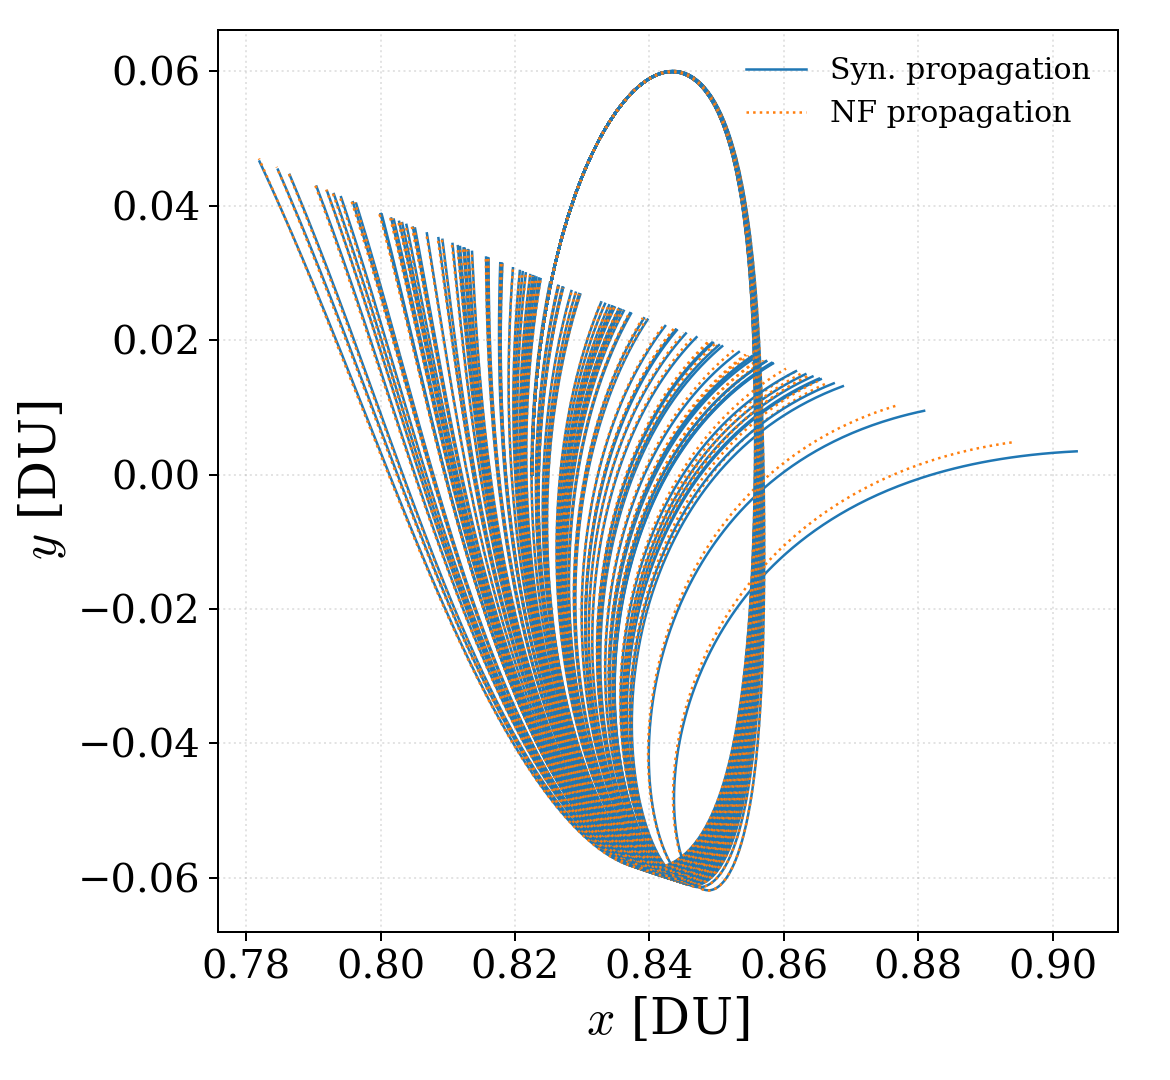
\includegraphics[height=5.3cm,keepaspectratio]{images/propagation_test_1_synodic_comparison_xy.png}
        \caption{Trajectories in $x$-$y$ space.}
        \label{fig:nf_traj}
    \end{subfigure}
    \hfill
    \begin{subfigure}{0.59\textwidth}
        \centering
        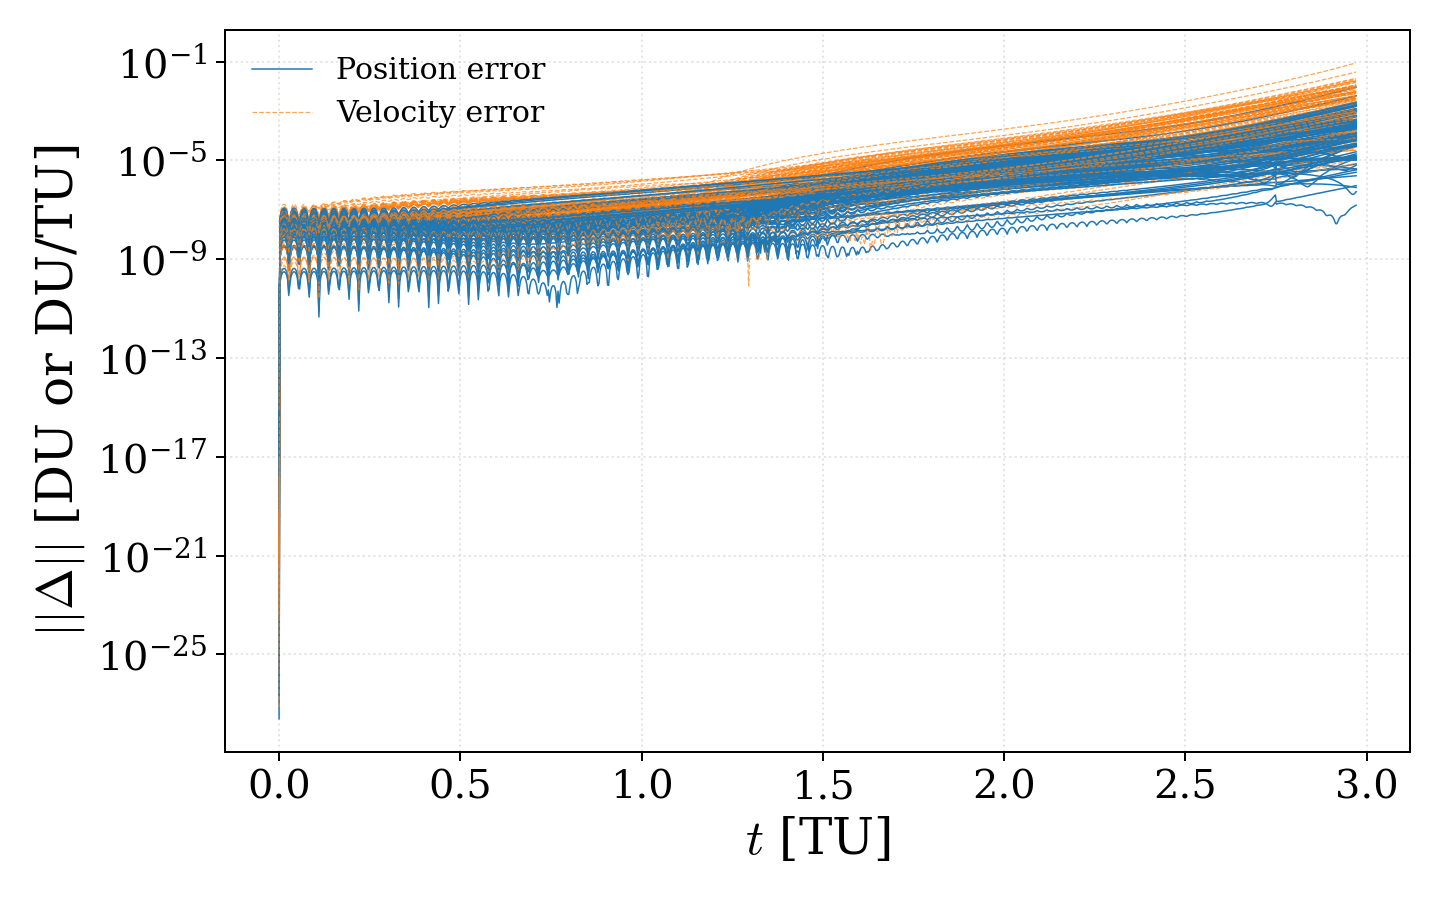
\includegraphics[height=5.3cm,keepaspectratio]{images/propagation_test_1_synodic_error.png}
        \caption{Position and velocity errors.}
        \label{fig:nf_err}
    \end{subfigure}

    \caption{Comparison of propagation in synodic and normal form coordinates.}
    \label{fig:nf_comparison}
\end{figure}

The left panel of \cref{fig:nf_comparison} compares the trajectories obtained with both propagation methods in the $x$-$y$ plane. 
Despite the small initial perturbations, the trajectories depart rapidly from the reference orbit over one period due to the strong instability of the Lyapunov orbit. 
Nevertheless, the normal form propagation closely follows the full synodic propagation while the trajectories remain near the reference orbit. 
As the trajectories move farther away, the accuracy decreases because the normal form is a local approximation; however, it still captures the qualitative behavior of the perturbed trajectories. 
This behavior is also reflected in the right panel, which shows the $L_2$ norms of the position and velocity errors over time for all propagated trajectories.

%\newpage %temporarily




% \clearpage
% \appendix
% \section{Appendix}    %%%Appendix probably not necessary, any proofs can probably jsut be in place, since it's a project/report.
% \label{app:appendix}

% \textcolor{red}{APPENDIX}





%\newpage

\addcontentsline{toc}{section}{Bibliography}

\bibliographystyle{alpha}  %use the plain bibliography style
% \nocite{*}
% \nocite{test1972}
\bibliography{references} % Entries are in the refs.bib file





\end{document}